\chapter{Prädikatenlogik}
In der \blue{Aussagenlogik} haben wir die Verknüpfung von atomaren Aussagen mit \blue{Junktoren} untersucht.
Die \blue{Prädikatenlogik}\index{Prädikatenlogik} untersucht zusätzlich auch die Struktur dieser atomaren Aussagen.  Dazu werden in der
Prädikatenlogik die folgenden zusätzlichen Begriffe eingeführt:
\begin{enumerate}
\item Als Bezeichnungen für Objekte werden \blue{Terme} verwendet.
\item Diese Terme werden aus \blue{Objekt-Variablen} und \blue{Funktions-Zeichen}
      zusammengesetzt.  In den folgenden Beispielen ist $x$ eine Objekt-Variable\index{Objekt-Variable}, während
      \textsl{vater} und \textsl{mutter} einstellige Funktions-Zeichen\index{Funktions-Zeichen}
      sind. \textsl{issac} ist ein nullstelliges Funktions-Zeichen:
      \\[0.2cm]
      \hspace*{1.3cm}
      $\textsl{vater}(x),\quad \textsl{mutter}(\textsl{isaac})$.
      \\[0.2cm]
      Nullstellige Funktions-Zeichen werden im Folgenden auch als \blue{Konstanten}\index{Konstante} bezeichnet
      und an Stelle von Objekt-Variablen reden wir kürzer nur von Variablen.
\item Verschiedene Objekte werden durch \blue{Prädikats-Zeichen}\index{Prädikats-Zeichen} in Relation gesetzt.
      In den folgenden Beispielen benutzen wir die Prädikats-Zeichen \textsl{istBruder} und $<$:
      \\[0.2cm]
      \hspace*{1.3cm}
      $\textsl{istBruder}\bigl(\textsl{albert}, \textsl{vater}(\textsl{bruno})\bigr),\quad x+7 < x\cdot 7$.
      \\[0.2cm]
      Die dabei entstehenden Formeln werden als \blue{atomare Formeln} \index{atomare Formeln} bezeichnet.
\item Atomare Formeln lassen sich durch aussagenlogische Junktoren verknüpfen:
      \\[0.2cm]
      \hspace*{1.3cm}
      $x > 1 \rightarrow x + 7 < x \cdot  7$.
\item Schließlich werden \blue{Quantoren}\index{Quantoren} eingeführt, um zwischen \blue{existentiell} und
      \blue{universell} quantifizierten Variablen unterscheiden
      zu können:
      \\[0.2cm]
      \hspace*{1.3cm}
      $\forall x \in \mathbb{R}: \exists n \in \mathbb{N}: x < n$.
\end{enumerate}
Dieses Kapitel ist wie folgt aufgebaut:
\begin{enumerate}[(a)]
\item Wir werden im nächsten Abschnitt die \href{https://de.wikipedia.org/wiki/Syntax}{Syntax} der
      prädikatenlogischen Formeln festlegen, wir werden also festlegen, welche Strings wir als aussagenlogische
      Formeln zulassen.
\item Im darauf folgenden Abschnitt beschäftigen wir uns mit der
      \href{https://de.wikipedia.org/wiki/Semantik}{Semantik} dieser Formeln, dort spe\-zifizieren wir also die 
      Bedeutung der Formeln. 
\item Danach zeigen wir, wie sich die eingeführten Begriffe in \textsl{Python} implementieren lassen.
\item Anschließend diskutieren wir als Anwendung der Prädikaten-Logik das \blue{Constraint Programming}.
      Beim Constraint Programming wird ein gegebenes Problem durch prädikatenlogische Formeln beschrieben.
      Zur Lösung des Problems wird dann ein sogenannter \blue{Constraint Solver} verwendet.
\item Weiter betrachten wir Normalformen prädikatenlogischer Formeln und zeigen, wie Formeln
      in \blue{erfüllbarkeits-äquivalente} prädikatenlogische Klauseln umgewandelt werden können.
\item Außerdem diskutieren wir einen \blue{prädikatenlogischen Kalkül}, der die Grundlage
      des automatischen Beweisens in der Prädikaten-Logik ist.
\item Zum Abschluss des Kapitels diskutieren wir den automatischen Theorem-Beweiser \textsl{Prover9}, sowie das
      Werkzeug \textsl{Mace4}, mit dem die Erfüllbarkeit von Formeln überprüft werden kann.
\end{enumerate}

\section{Syntax der Prädikatenlogik}
Zunächst definieren wir den Begriff der \blue{Signatur}\index{Signatur}. Inhaltlich ist das nichts anderes als
eine strukturierte Zusammenfassung von Variablen, Funktions- und Prädikats-Zeichen zusammen mit
einer Spezifikation der Stelligkeit dieser Zeichen.
 
\begin{Definition}[Signatur]
  Eine \blue{Signatur} ist ein 4-Tupel \\[0.2cm]
  \hspace*{1.3cm} $\Sigma = \langle \mathcal{V}, \mathcal{F}, \mathcal{P}, \textsl{arity} \rangle$, \\[0.2cm]
  für das Folgendes gilt: 
  \begin{enumerate}
  \item $\mathcal{V}$ ist die Menge der \blue{Objekt-Variablen},\index{Objekt-Variablen} die wir der Kürze halber meist nur als
        \blue{Variablen} be\-zeichnen.
  \item $\mathcal{F}$ ist die Menge der \blue{Funktions-Zeichen}.\index{Funktions-Zeichen}
  \item $\mathcal{P}$ ist die Menge der \blue{Prädikats-Zeichen}.\index{Prädikats-Zeichen}
  \item $\textsl{arity}$ ist eine Funktion, die jedem Funktions- und jedem Prädikats-Zeichen seine
        \blue{Stelligkeit}\index{Stelligkeit} zuordnet: \\[0.2cm]
        \hspace*{1.3cm} $\textsl{arity}: \mathcal{F} \cup \mathcal{P} \rightarrow \mathbb{N}$. \\[0.2cm]
        Wir sagen, dass das Funktions- oder Prädikats-Zeichen $f$ ein
        $n$-stelliges Zeichen ist, falls $\textsl{arity}(f) = n$ gilt.
  \item Da wir in der Lage sein müssen, Variablen, Funktions- und Prädikats-Zeichen
        unterscheiden zu können, vereinbaren wir, dass die Mengen $\mathcal{V}$,
        $\mathcal{F}$ und $\mathcal{P}$ paarweise disjunkt sein müssen: \\[0.2cm] 
        \hspace*{1.3cm} $\mathcal{V} \cap \mathcal{F} = \{\}$, \quad
                        $\mathcal{V} \cap \mathcal{P} = \{\}$, \quad und \quad
                        $\mathcal{F} \cap \mathcal{P} = \{\}$. \eox
  \end{enumerate}
\end{Definition}

\noindent
Als Bezeichner für Objekte verwenden wir Ausdrücke, die aus Variablen und
Funktions-Zeichen aufgebaut sind.  Solche Ausdrücke nennen wir \blue{Terme}.\index{Terme}  

\begin{Definition}[Terme,  $\mathcal{T}_\Sigma$]
  Ist $\Sigma = \langle \mathcal{V}, \mathcal{F}, \mathcal{P}, \textsl{arity} \rangle$ eine Signatur, so definieren wir die Menge der \blue{$\Sigma$-Terme}
  \blue{$\mathcal{T}_\Sigma$} \index{$\mathcal{T}_\Sigma$} induktiv:
  \begin{enumerate}
  \item Für jede Variable $x \in \mathcal{V}$ gilt $x \in \mathcal{T}_\Sigma$.  Jede Variable ist also auch
        ein Term.
  \item Ist $f \in \mathcal{F}$ ein n-stelliges Funktions-Zeichen und sind 
        $t_1,\cdots,t_n \el \mathcal{T}_\Sigma$, so gilt 
        \\[0.2cm]
        \hspace*{1.3cm} $f(t_1,\cdots,t_n) \el \mathcal{T}_\Sigma$,
        \\[0.2cm]
        der Ausdruck  $f(t_1,\cdots,t_n) \el \mathcal{T}_\Sigma$ ist also ein Term.
        Falls $c \in \mathcal{F}$ ein 0-stelliges Funktions-Zeichen ist, lassen wir auch die Schreibweise
        $c$ anstelle von $c()$ zu.  In diesem Fall nennen wir $c$ eine \blue{Konstante}.\index{Konstante}
        \eox
  \end{enumerate}
\end{Definition}

\example
Es sei 
\begin{enumerate}
\item $\mathcal{V} := \{ x, y, z \}$ die Menge der Variablen,
\item $\mathcal{F} := \{ 0, 1, \mathtt{+}, \mathtt{-}, * \}$ die Menge der Funktions-Zeichen,
\item $\mathcal{P} := \{\mathtt{=}, \leq\}$ die Menge der Prädikats-Zeichen,
\item $\textsl{arity} := \bigl\{ 0 \mapsto 0, 1 \mapsto 0, \mathtt{+} \mapsto 2, \mathtt{-} \mapsto 2,
                                 * \mapsto 2, = \;\mapsto 2, \leq\; \mapsto 2 \bigr\}$, \\[0.2cm]
      gibt die Stelligkeit der Funktions- und Prädikats-Zeichen an und
\item $\Sigma_\mathrm{arith} := \langle \mathcal{V}, \mathcal{F}, \mathcal{P}, \textsl{arity} \rangle$
      sei eine Signatur.
\end{enumerate}
Dann können wir wie folgt $\Sigma_{\mathrm{arith}}$-Terme konstruieren:
\begin{enumerate}
\item $x, y, z \in \mathcal{T}_{\Sigma_{\mathrm{arith}}}$, \\[0.2cm]
      denn alle Variablen sind auch $\Sigma_{\mathrm{arith}}$-Terme.
\item $0, 1 \in \mathcal{T}_{\Sigma_{\mathrm{arith}}}$,  \\[0.2cm]
      denn $0$ und $1$ sind $0$-stellige Funktions-Zeichen.
\item $\mathtt{+}(0,x) \in \mathcal{T}_{\Sigma_{\mathrm{arith}}}$, \\[0.2cm]
      denn es gilt $0 \in \mathcal{T}_{\Sigma_{\mathrm{arith}}}$, $x \in \mathcal{T}_{\Sigma_{\mathrm{arith}}}$ und 
      $\mathtt{+}$ ist ein 2-stelliges Funktions-Zeichen.
\item $*(\mathtt{+}(0,x),1) \in \mathcal{T}_{\Sigma_{\mathrm{arith}}}$, \\[0.2cm]
      denn $\mathtt{+}(0,x) \in \mathcal{T}_{\Sigma_{\mathrm{arith}}}$, $1 \in \mathcal{T}_{\Sigma_{\mathrm{arith}}}$ und
      $*$ ist ein 2-stelliges Funktions-Zeichen.
\end{enumerate}
In der Praxis werden wir für bestimmte zweistellige Funktionen eine \blue{Infix-Schreibweise}
verwenden, d.h.~wir schreiben zweistellige Funktions-Zeichen zwischen ihren Argumenten.  Beispielsweise
schreiben wir $x+y$ an Stelle von $+(x,y)$. Die Infix-Schreibweise ist dann als Abkürzung für die oben
definierte Darstellung zu verstehen.  Dies funktioniert natürlich nur, wenn wir für die einzelnen Operatoren
auch Bindungsstärken festlegen. 
\eox


Als nächstes definieren wir den Begriff der \blue{atomaren Formeln}.\index{Atomare Formeln}  Darunter verstehen
wir solche Formeln, die man nicht in kleinere Formeln zerlegen kann: Atomare Formeln enthalten also
weder Junktoren noch Quantoren. 
\begin{Definition}[Atomare Formeln,  $\mathcal{A}_\Sigma$]
  Gegeben sei eine Signatur $\Sigma = \langle \mathcal{V}, \mathcal{F}, \mathcal{P}, \textsl{arity} \rangle$. 
  Die Menge der atomaren $\Sigma$-Formeln $\mathcal{A}_\Sigma$ \index{$\mathcal{A}_\Sigma$}
  wird wie folgt definiert:  Ist $p \el \mathcal{P}$ ein $n$-stelliges Prädikats-Zeichen
  und sind $n$ $\Sigma$-Terme $t_1$, $\cdots$, $t_n$ gegeben, so ist
  $p(t_1,\cdots,t_n)$ eine \blue{atomaren $\Sigma$-Formel}: \\[0.2cm]
  \hspace*{1.3cm} $p(t_1,\cdots,t_n) \in \mathcal{A}_\Sigma$.  \\[0.2cm]
  Falls $p$ ein 0-stelliges Prädikats-Zeichen ist, dann schreiben wir auch $p$ anstelle von $p()$.
  In diesem Fall nennen wir $p$ eine \blue{Aussage-Variable}.\index{Aussage-Variable}
  \eox
\end{Definition}

\example
Setzen wir das letzte Beispiel fort, so können wir sehen, dass \\[0.2cm]
\hspace*{1.3cm} $\mathtt{=}(*(\mathtt{+}(0,x),1),0)$ \\[0.2cm]
eine atomare $\Sigma_\mathrm{arith}$-Formel ist.  Beachten Sie, dass wir bisher noch nichts über den Wahrheitswert von solchen 
Formeln ausgesagt haben.  Die Frage, wann eine Formel als wahr oder falsch gelten soll,
wird erst im nächsten Abschnitt untersucht.
\eox


Bei der Definition der prädikatenlogischen Formeln ist es notwendig,
zwischen sogenannten \blue{gebundenen}\index{gebundene Variable} und \blue{freien}
Variablen \index{freie Variable} zu unterscheiden. 
Wir führen diese Begriffe zunächst informal mit Hilfe eines Beispiels aus der Analysis ein.
Wir betrachten die folgende Gleichung: \\[0.2cm]
\hspace*{1.3cm}
 $\ds\int_{0}^{x} y \cdot  t\, d t = \frac{1}{2} \cdot x^2 \cdot  y$ 
\\[0.2cm]
In dieser Gleichung treten die Variablen $x$ und $y$ \blue{frei} auf, während die Variable $t$ durch das Integral
\blue{gebunden} wird.  Damit meinen wir folgendes: Wir können in dieser Gleichung für $x$ und $y$ beliebige Werte
 einsetzen, ohne dass sich an der 
Gültigkeit der Formel etwas ändert.  Setzen wir zum Beispiel für $x$ den Wert $2$ ein, so erhalten wir \\[0.2cm]
\hspace*{1.3cm}
$\ds\int_{0}^{2} y \cdot  t\, d t = \frac{1}{2} \cdot 2^2 \cdot  y$ \\[0.2cm]
und diese Gleichung ist ebenfalls gültig.  Demgegenüber macht es keinen Sinn, wenn wir für die gebundene Variable
 $t$ eine Zahl einsetzen würden.
Die linke Seite der entstehenden Gleichung wäre einfach undefiniert.  Wir können für $t$
höchstens eine andere Variable einsetzen. 
Ersetzen wir die Variable $t$ beispielsweise durch $u$, so erhalten wir \\[0.2cm]
\hspace*{1.3cm}
$\ds\int_{0}^{x} y \cdot  u\, d u = \frac{1}{2} \cdot x^2 \cdot  y$ 
\\[0.2cm]
und das ist inhaltlich dieselbe Aussage wie oben.  Das funktioniert allerdings nicht mit jeder Variablen. Setzen wir
für $t$ die Variable $y$ ein, so erhalten wir \\[0.2cm]
\hspace*{1.3cm}
$\ds\int_{0}^{x} y \cdot  y\, d y = \frac{1}{2} \cdot x^2 \cdot  y$. \\[0.2cm]
Diese Aussage ist aber falsch!  Das Problem liegt darin, dass bei der Ersetzung von $t$ durch $y$ die vorher freie Variable
$y$ gebunden wurde.  

Ein ähnliches Problem erhalten wir, wenn wir für $y$ beliebige Terme einsetzen.  Solange diese Terme die Variable $t$ 
nicht enthalten, geht alles gut.  Setzen wir beispielsweise für $y$  den Term $x^2$ ein, so erhalten
wir \\[0.2cm]
\hspace*{1.3cm}
$\ds\int_{0}^{x} x^2 \cdot  t\, d t = \frac{1}{2} \cdot x^2 \cdot  x^2$ 
\\[0.2cm]
und diese Formel ist gültig.  Setzen wir allerdings für $y$ den Term $t^2$ ein, so erhalten wir \\[0.2cm]
\hspace*{1.3cm}
$\ds\int_{0}^{x} t^2 \cdot  t\, d t = \frac{1}{2} \cdot x^2 \cdot  t^2$ 
\\[0.2cm]
und diese Formel ist nicht mehr gültig. 

In der Prädikatenlogik binden die Quantoren ``$\forall$'' (\blue{für alle}) und ``$\exists$''
(\blue{es gibt}) Variablen in ähnlicher Weise,  wie der Integral-Operator ``$\int \cdot\; \mathtt{d}t$'' in
der Analysis Variablen bindet.  Die oben gemachten Ausführungen zeigen, dass es zwei verschiedene Arten von 
Variable gibt: \blue{freie Variablen} und \blue{gebundene Variablen}.
Um diese Begriffe präzisieren zu können, definieren wir zunächst für einen
$\Sigma$-Term $t$ die Menge der in $t$ enthaltenen Variablen.

\begin{Definition}[$\var(t)$]
  \index{$\var(t)$}
  Ist $\Sigma = \langle \mathcal{V}, \mathcal{F}, \mathcal{P}, \textsl{arity} \rangle$ eine Signatur und ist
  $t$ ein $\Sigma$-Term, so definieren wir die Menge \blue{$\var(t)$} der Variablen, die in $t$
    auftreten, durch Induktion nach dem Aufbau des Terms:
    \begin{enumerate}
    \item $\var(x) := \{ x \}$ \quad für alle $x \in \mathcal{V}$,
    \item $\var\bigl(f(t_1,\cdots,t_n)\bigr) := \var(t_1) \cup \cdots \cup \var(t_n)$.
          \eox
    \end{enumerate}
\end{Definition}


\begin{Definition}[$\Sigma$-Formel,  $\mathbb{F}_\Sigma$, gebundene und freie Variablen, $\textsl{BV}(F)$,  $\textsl{FV}(F)$] 
\label{praedikaten-formel} \hspace*{\fill} 
\index{$\Sigma$-Formel} \index{$\mathbb{F}_\Sigma$}\index{gebundene Variablen}\index{freie
  Variablen}\index{$\textsl{BV}(F)$}\index{$\textsl{FV}(F)$} \\
Es sei $\Sigma = \langle \mathcal{V}, \mathcal{F}, \mathcal{P}, \textsl{arity} \rangle$ eine Signatur.
    Die Menge der {\color{blue}$\Sigma$-\emph{Formeln}} bezeichnen wir mit $\mathbb{F}_\Sigma$.
    Wir definieren diese Menge induktiv.
    Gleichzeitig definieren wir für jede Formel $F\el \mathbb{F}_\Sigma$ die Menge $\textsl{BV}(F)$ der in $F$ 
    \blue{gebunden} auftretenden Variablen und die Menge $\textsl{FV}(F)$ der in $F$ \blue{frei} auftretenden Variablen.
    \begin{enumerate}
    \item Es gilt $\falsum \in \mathbb{F}_\Sigma$ und $\verum \in \mathbb{F}_\Sigma$ und wir definieren \\[0.2cm]
          \hspace*{1.3cm} $\FV(\falsum) := \FV(\verum) := \BV(\falsum) := \BV(\verum) := \{\}$.
    \item Ist $F = p(t_1,\cdots,t_n)$ eine atomare $\Sigma$-Formel, so gilt $F \in \mathbb{F}_\Sigma$.  Weiter definieren wir:
          \begin{enumerate}
          \item $\FV\bigl(p(t_1,\cdots,t_n) \bigr) := \var(t_1) \cup \cdots \cup \var(t_n)$.
          \item $\BV\bigl(p(t_1,\cdots,t_n) \bigr) := \{\}$.
          \end{enumerate}
    \item Ist $F \in \mathbb{F}_\Sigma$, so gilt $\neg F \in \mathbb{F}_\Sigma$. Weiter definieren wir:
          \begin{enumerate}
          \item $\FV\bigl( \neg F \bigr) := \FV(F)$.
          \item $\BV\bigl( \neg F \bigr) := \BV(F)$.
          \end{enumerate}
    \item Sind $F, G \in \mathbb{F}_\Sigma$ und gilt außerdem \\[0.2cm]
          \hspace*{1.3cm}
          $\bigl(\FV(F) \cup \FV(G)\bigr) \cap \bigl(\BV(F) \cup \BV(G)) = \{\}$,
          \\[0.2cm]
          so gilt auch
          \begin{enumerate}
          \item $(F \wedge G) \in \mathbb{F}_\Sigma$,
          \item $(F \vee G) \in \mathbb{F}_\Sigma$,
          \item $(F \rightarrow G) \in \mathbb{F}_\Sigma$,
          \item $(F \leftrightarrow G) \in \mathbb{F}_\Sigma$.
          \end{enumerate}
          Weiter definieren wir für alle Junktoren $\odot \in \{ \wedge, \vee, \rightarrow, \leftrightarrow \}$:
          \begin{enumerate}
          \item $\FV\bigl((F \odot G) \bigr) := \FV(F) \cup \FV(G)$.
          \item $\BV\bigl((F \odot G) \bigr) := \BV(F) \cup \BV(G)$.
          \end{enumerate}
    \item Sei $x \in \mathcal{V}$  und $F \in \mathbb{F}_\Sigma$ mit $x \not\in \BV(F)$.  Dann gilt:
          \begin{enumerate}
          \item $(\forall x \colon F) \in \mathbb{F}_\Sigma$.
          \item $(\exists x \colon F) \in \mathbb{F}_\Sigma$.
          \end{enumerate}
          Weiter definieren wir 
          \begin{enumerate}
          \item $\FV\bigl( (\forall x \colon F) \bigr) := \FV\bigl( (\exists x \colon F) \bigr) := \FV(F) \backslash \{x\}$.
          \item $\BV\bigl( (\forall x \colon F) \bigr) := \BV\bigl( (\exists x \colon F) \bigr) := \BV(F) \cup \{x\}$.  
          \end{enumerate}
    \end{enumerate}
    Ist die Signatur $\Sigma$ aus dem Zusammenhang klar oder aber unwichtig, so schreiben wir
    auch $\mathbb{F}$ statt $\mathbb{F}_\Sigma$ und sprechen dann einfach von Formeln statt von $\Sigma$-Formeln.
    \eox
\end{Definition}

Bei der oben gegebenen Definition haben wir darauf geachtet, dass eine Variable nicht gleichzeitig
frei und gebunden in einer Formel auftreten kann, denn durch eine leichte Induktion nach dem Aufbau
der Formeln lässt sich zeigen, dass für alle $F \in \mathbb{F}_\Sigma$ folgendes gilt:
\\[0.2cm]
\hspace*{1.3cm}
$ \FV(F) \cap \BV(F) = \{\}$. 


\example
Setzen wir das oben begonnene Beispiel fort, so  sehen wir, dass \\[0.2cm]
\hspace*{1.3cm} $(\exists x \colon\, \leq\!(\mathtt{+}(y, x),y))$ \\[0.2cm]
eine Formel aus $\mathbb{F}_{\Sigma_{\mathrm{arith}}}$ ist. 
Die Menge der gebundenen Variablen ist $\{x\}$, die Menge der freien Variablen ist 
$\{ y \}$. \eox

Wenn wir Formeln immer in der oben definierten Präfix-Notation anschreiben würden, dann würde die Lesbarkeit unverhältnismäßig leiden. 
Zur Abkürzung vereinbaren wir, dass in der Prä\-dikatenlogik dieselben Regeln zur Klammer-Ersparnis
gelten sollen,  die wir schon in der Aussagenlogik verwendet haben.  Zusätzlich werden
gleiche Quantoren zusammengefasst: Beispielsweise schreiben wir  
\\[0.2cm]
\hspace*{1.3cm}
$\forall x, y \colon p(x, y)  \quad \mathrm{statt} \quad \forall x \colon ( \forall y \colon p(x,y))$.
\\[0.2cm]
Außerdem vereinbaren wir, dass wir zweistellige Prädikats- und Funktions-Zeichen auch in Infix-Notation angeben
dürfen.  Um eine eindeutige Lesbarkeit zu erhalten, müssen wir dann die Präzedenz der Funktions-Zeichen
festlegen.  Wir schreiben beispielsweise \\[0.2cm]
\hspace*{1.3cm} $\mathtt{n}_1 = \mathtt{n}_2$  \quad anstelle von \quad $=(\mathtt{n}_1, \mathtt{n}_2)$. \\[0.2cm]
Die Formel $(\exists x \colon \leq(\mathtt{+}(y, x),y))$ wird dann lesbarer als \\[0.2cm]
\hspace*{1.3cm} $\exists x \colon y + x \leq y$ \\[0.2cm]
geschrieben.  Außerdem finden Sie in der Literatur häufig Ausdrücke der Form
\\[0.2cm]
\hspace*{1.3cm}
$\forall x\el M: F$ \quad oder \quad $\exists x\el M: F$.
\\[0.2cm]
Hierbei handelt es sich um Abkürzungen, die durch
\\[0.2cm]
\hspace*{1.3cm}
$\ds \bigl(\forall x\el M: F\bigr) \stackrel{\mathrm{def}}{\Longleftrightarrow} \forall x: \bigl(x \el M \rightarrow F\bigr)$,
\quad und \quad 
$\ds\bigl(\exists x\el M: F\bigr) \stackrel{\mathtt{def}}{\Longleftrightarrow} \exists x: \bigl(x \el M \wedge F\bigr)$.
\\[0.2cm]
definiert sind.

\section{Semantik der Prädikatenlogik \label{sec:semantik}}
Als nächstes legen wir die Bedeutung der Formeln fest.  Dazu definieren wir 
den Begriff einer \blue{$\Sigma$-Struktur}. \index{$\Sigma$-Struktur}  Eine solche Struktur legt fest, wie die
Funktions- und Prädikats-Zeichen der Signatur $\Sigma$ zu interpretieren sind.

\begin{Definition}[Struktur]
    Es sei eine  Signatur \\[0.2cm]
    \hspace*{1.3cm} $\Sigma = \langle \mathcal{V}, \mathcal{F}, \mathcal{P}, \textsl{arity} \rangle$. \\[0.2cm]
    gegeben. Eine \blue{$\Sigma$-Struktur} $\struct$ ist ein
    Paar $\langle \mathcal{U}, \mathcal{J} \rangle$, so dass folgendes gilt:
    \begin{enumerate}
        \item $\mathcal{U}$ ist eine nicht-leere Menge. Diese Menge nennen wir auch das
              \blue{Universum} \index{Universum} der $\Sigma$-Struktur.  Dieses Universum enthält die Werte,
              die sich später bei der Auswertung der Terme ergeben werden.
        \item $\mathcal{J}$ ist die \blue{Interpretation} \index{Interpretation} der Funktions-- und Prädikats-Zeichen.
              Formal definieren wir $\mathcal{J}$ als eine Abbildung mit folgenden Eigenschaften:
        \begin{enumerate}
        \item Jedem Funktions-Zeichen $f \el \mathcal{F}$ mit $\textsl{arity}(f) = m$ wird
              eine $m$-stellige Funktion \\[0.2cm]
              \hspace*{1.3cm}
              $f^\mathcal{J}\colon \mathcal{U}^m \rightarrow \mathcal{U}$ \\[0.2cm]
              zugeordnet, die $m$-Tupel des Universums $\mathcal{U}$ in das Universum $\mathcal{U}$ abbildet.
        \item Jedem Prädikats-Zeichen $p \el \mathcal{P}$ mit $\textsl{arity}(p) = n$ wird
              eine Teilmenge \\[0.2cm]
              \hspace*{1.3cm} 
              $p^\mathcal{J} \subseteq \mathcal{U}^n$ \\[0.2cm]
              zugeordnet.  Die Idee ist, dass eine atomare Formel der Form $p(t_1, \cdots, t_n)$
              genau dann als wahr interpretiert wird, wenn die Interpretation des Tupels
              $\langle t_1, \cdots, t_n \rangle$ ein Element der Menge $p^\mathcal{J}$ ist.
        \item Ist das Zeichen ``$=$'' ein Element der Menge der Prädikats-Zeichen $\mathcal{P}$, so gilt
              \\[0.2cm]
              \hspace*{1.3cm}  
              $=^\mathcal{J} \;=\; \bigl\{ \langle u, u \rangle \mid u \in \mathcal{U} \bigr\}$.
              \\[0.2cm]
              Eine Formel der Art $s = t$ wird also genau dann als wahr interpretiert, 
              wenn die Interpretation des Terms $s$ den selben Wert ergibt wie die Interpretation des Terms $t$.
              \eox
        \end{enumerate}
    \end{enumerate}
\end{Definition}

\example
Die Signatur  $\Sigma_G$ der Gruppen-Theorie sei definiert als \\[0.2cm]
\hspace*{1.3cm} $\Sigma_G = \langle \mathcal{V}, \mathcal{F}, \mathcal{P},\textsl{arity}\rangle$ 
\quad mit
\begin{enumerate}
\item $\mathcal{V} := \{ x, y, z \}$
\item $\mathcal{F} := \{ \mathrm{e}, * \}$
\item $\mathcal{P} := \{ \mathtt{=} \}$
\item $\textsl{arity} = \bigl\{ \pair(\mathrm{e},0), \pair(*,2), \pair(\mathtt{=},2)\bigr\}$
\end{enumerate}
Dann können wir eine $\Sigma_G$ Struktur $\mathcal{Z} = \langle \{0,1\},\mathcal{J}\rangle$ definieren, 
indem wir die Interpretation $\mathcal{J}$ 
wie folgt festlegen:
\begin{enumerate}
\item $\mathrm{e}^\mathcal{J} := 0$,
\item $*^\mathcal{J} := \Bigl\{ \bigl\langle\pair(0,0), 0\bigr\rangle,
                                   \bigl\langle\pair(0,1), 1\bigr\rangle,
                                   \bigl\langle\pair(1,0), 1\bigr\rangle,
                                   \bigl\langle\pair(1,1), 0\bigr\rangle \Bigr\}$,
\item $=^\mathcal{J} \;:=\; \bigl\{ \pair(0,0), \pair(1,1) \bigr\}$.
                                 
      Beachten Sie, dass wir bei der Interpretation des Gleichheits-Zeichens 
      keinen Spielraum haben! \eox
\end{enumerate}

Falls wir Terme auswerten wollen, die Variablen enthalten, so müssen wir für diese
Variablen irgendwelche Werte aus dem Universum einsetzen.  Welche Werte wir einsetzen, kann
durch eine \blue{Variablen-Belegung}\index{Variablen-Belegung} festgelegt werden.  Diesen Begriff definieren wir
nun.

\begin{Definition}[Variablen-Belegung]
    Es sei eine  Signatur \\[0.2cm]
    \hspace*{1.3cm} $\Sigma = \langle \mathcal{V}, \mathcal{F}, \mathcal{P}, \textsl{arity} \rangle$ \\[0.2cm]
    gegeben.  Weiter sei $\struct = \langle \mathcal{U}, \mathcal{J} \rangle$ eine $\Sigma$-Struktur.  Dann bezeichnen wir 
     eine Abbildung \\[0.2cm]
    \hspace*{1.3cm} $\mathcal{I}: \mathcal{V} \rightarrow \mathcal{U}$ \\[0.2cm]
    als eine {\color{blue}$\struct$-\emph{Variablen-Belegung}}.

    Ist $\mathcal{I}$ eine $\struct$-Variablen-Belegung,
    $x \in \mathcal{V}$ und $c \in \mathcal{U}$, so bezeichnet \blue{$\mathcal{I}[x/c]$} die Variablen-Belegung, die 
    der Variablen $x$ den Wert $c$ zuordnet und die ansonsten mit $\mathcal{I}$ übereinstimmt: \\[0.2cm]
    \hspace*{1.3cm} 
    $\mathcal{I}[x/c](y) := \left\{
    \begin{array}{ll}
    c               & \mbox{falls}\; y = x;  \\
    \mathcal{I}(y)  & \mbox{sonst}.          \\
    \end{array}
    \right.$ \eox
\end{Definition}


\begin{Definition}[Semantik der Terme]
    Ist $\struct = \pair(\mathcal{U},\mathcal{J})$ eine $\Sigma$-Struktur und $\mathcal{I}$ eine $\struct$-Variablen-Belegung,
    so definieren wir für jeden Term $t$ den \blue{Wert} \blue{$\struct(\mathcal{I}, t)$}
    \index{$\struct(\mathcal{I}, t)$} durch Induktion über
    den Aufbau von $t$:
    \begin{enumerate}
    \item Für Variablen $x \in \mathcal{V}$ definieren wir: \\[0.2cm]
          \hspace*{1.3cm} $\struct(\mathcal{I}, x) := \mathcal{I}(x)$.
    \item Für $\Sigma$-Terme der Form $f(t_1,\cdots,t_n)$ definieren wir \\[0.2cm]
          \hspace*{1.3cm} $\struct\bigl(\mathcal{I}, f(t_1,\cdots,t_n)\bigr) := 
                           f^\mathcal{J}\bigl( \struct(\mathcal{I}, t_1), \cdots, \struct(\mathcal{I}, t_n) \bigr)$.
                           \eox
    \end{enumerate}
\end{Definition}

\example
Mit der oben definieren $\Sigma_G$-Struktur
$\mathcal{Z}$ definieren wir eine $\mathcal{Z}$-Variablen-Belegung $\mathcal{I}$ durch
\\[0.2cm]
\hspace*{1.3cm} $\mathcal{I} := \bigl\{ \pair(x,0), \pair(y,1), \pair(z,0)\bigr\}$,
\\[0.2cm]
es gilt also
\\[0.2cm]
\hspace*{1.3cm} $\mathcal{I}(\mathtt{x}) := 0$, \quad $\mathcal{I}(\mathtt{y}) := 1$, \quad und \quad $\mathcal{I}(\mathtt{z}) := 0$.
\\[0.2cm]
Dann gilt  \\[0.2cm]
\hspace*{1.3cm}  $\mathcal{Z}\bigl(\mathcal{I}, \mathtt{x} * \mathtt{y} \bigr) = 1$. \eox

\begin{Definition}[Semantik der atomaren $\Sigma$-Formeln]
    Ist $\struct$ eine $\Sigma$-Struktur und $\mathcal{I}$ eine $\struct$-Variablen-Belegung,
    so definieren wir für jede atomare $\Sigma$-Formel 
    $p(t_1, \cdots, t_n)$ den Wert \blue{$\struct\bigl(\mathcal{I}, p(t_1, \cdots, t_n) \bigr)$} wie folgt: \\[0.2cm]
    \hspace*{1.3cm}
    $\struct\bigl(\mathcal{I}, p(t_1,\cdots,t_n)\bigr) := 
       \Bigl(\bigl\langle \struct(\mathcal{I}, t_1), \cdots, \struct(\mathcal{I}, t_n) \bigr\rangle \in p^\mathcal{J}\Bigr)$.
    \eox
\end{Definition}

\example
In Fortführung des obigen Beispiels gilt: 
\\[0.2cm]
\hspace*{1.3cm} 
$\mathcal{Z}(\mathcal{I},x * y = y * x) = \mathtt{True}$.
\eox

Um die Semantik beliebiger $\Sigma$-Formeln definieren zu können, nehmen wir an, dass wir,
genau wie in der Aussagenlogik, die folgenden Funktionen zur Verfügung haben:
\begin{enumerate}
\item $\circneg: \mathbb{B} \rightarrow \mathbb{B}$,
\item $\circvee: \mathbb{B} \times \mathbb{B} \rightarrow \mathbb{B}$,
\item $\circwedge: \mathbb{B} \times \mathbb{B} \rightarrow \mathbb{B}$,
\item $\circright: \mathbb{B} \times \mathbb{B} \rightarrow \mathbb{B}$,
\item $\circleftright: \mathbb{B} \times \mathbb{B} \rightarrow \mathbb{B}$.
\end{enumerate}
Die Semantik dieser Funktionen hatten wir durch die Tabelle in Abbildung
\ref{tab:aussagen-logik} auf Seite \pageref{tab:aussagen-logik} gegeben. 

\begin{Definition}[Semantik der $\Sigma$-Formeln]
    Ist $\struct$ eine $\Sigma$-Struktur und $\mathcal{I}$ eine $\struct$-Variablen-Belegung,
    so definieren wir für jede $\Sigma$-Formel $F$ den Wert \blue{$\struct(\mathcal{I},F)$}
    durch Induktion über den Aufbau von $F$:
    \begin{enumerate}
    \item $\struct(\mathcal{I},\verum) := \mathtt{True}$ und $\struct(\mathcal{I},\falsum) := \mathtt{False}$.
    \item $\struct(\mathcal{I}, \neg F) \;:=\; \circneg\bigl(\struct(\mathcal{I}, F)\bigr)$.
    \item $\struct(\mathcal{I}, F \wedge G) \;:=\; \circwedge\bigl(\struct(\mathcal{I}, F), \struct(\mathcal{I}, G)\bigr)$.
    \item $\struct(\mathcal{I}, F \vee G) \;:=\; \circvee\bigl(\struct(\mathcal{I}, F), \struct(\mathcal{I}, G)\bigr)$.
    \item $\struct(\mathcal{I}, F \rightarrow G) \;:=\; \circright\!\bigl(\struct(\mathcal{I}, F), \struct(\mathcal{I}, G)\bigr)$.
    \item $\struct(\mathcal{I}, F \leftrightarrow G) \;:=\; \circleftright\bigl(\struct(\mathcal{I}, F), \struct(\mathcal{I}, G)\bigr)$.
    \item $\struct\bigl(\mathcal{I}, \forall x\colon F\bigr) \;:=\; \left\{
      \begin{array}{ll}
         \mathtt{True}  & \mbox{falls}\; \struct(\mathcal{I}[x/c], F) = \mathtt{True}\quad \mbox{für alle}\; c\in \mathcal{U}\;\mbox{gilt}; \\
         \mathtt{False} & \mbox{sonst}.
      \end{array}
      \right.$
    \item $\struct\bigl(\mathcal{I}, \exists x \colon F\bigr) \;:=\; \left\{
      \begin{array}{ll}
         \mathtt{True}  & \mbox{falls}\; \struct(\mathcal{I}[x/c], F) = \mathtt{True}\quad \mbox{für ein}\; c\in \mathcal{U}\;\mbox{gilt}; \\
         \mathtt{False} & \mbox{sonst}.
      \end{array}
      \right.$\eox    
    \end{enumerate}
\end{Definition}

\example
In Fortführung des obigen Beispiels gilt \\[0.2cm]
\hspace*{1.3cm}  $\mathcal{Z}\bigl(\mathcal{I}, \forall \mathtt{x}: \mathrm{e} * x = x \bigr) = \mathtt{True}$.
\eox

\begin{Definition}[Allgemeingültig] \index{Allgemeingültig}
    Ist $F$ eine $\Sigma$-Formel, so dass für jede $\Sigma$-Struktur $\struct$ und für jede
    $\struct$-Variablen-Belegung $\mathcal{I}$ \\[0.2cm]
    \hspace*{1.3cm} $\struct(\mathcal{I}, F) = \mathtt{True}$ \\[0.2cm]
    gilt, so bezeichnen wir $F$ als \blue{allgemeingültig}.  In diesem Fall schreiben wir \\[0.2cm]
    \hspace*{1.3cm} $\models F$. 
    \eox
\end{Definition}

Ist $F$ eine Formel für die $\FV(F) = \{\}$ ist, dann hängt der Wert $\struct(\mathcal{I}, F)$ 
offenbar gar nicht von der Interpretation $\mathcal{I}$ ab.  Solche Formeln bezeichnen wir auch als 
\blue{geschlossene} Formeln.\index{geschlossene Formel}   In diesem Fall schreiben wir kürzer  $\struct(F)$
an Stelle von $\struct(\mathcal{I}, F)$.  Gilt dann zusätzlich $\struct(F) = \mathtt{True}$, 
so sagen wir auch, dass $\struct$ ein \blue{Modell} \index{Modell} von $F$ ist.  Wir schreiben dann \\[0.2cm]
\hspace*{1.3cm} $\mathcal{S} \models F$. \index{$\mathcal{S} \models F$}
\vspace{0.1cm}

Die Definition der Begriffe ``\blue{erfüllbar}'' und
``\blue{äquivalent}'' lassen sich nun aus der Aussagenlogik übertragen. 
Um unnötigen Ballast in den Definitionen zu vermeiden, nehmen wir im Folgenden immer eine
feste Signatur $\Sigma$ als gegeben an.  Dadurch können wir in den folgenden Definitionen
von Termen, Formeln, Strukturen, etc.~sprechen und meinen damit  $\Sigma$-Terme,
$\Sigma$-Formeln und $\Sigma$-Strukturen.

\begin{Definition}[Äquivalent] \index{äquivalent}
  Zwei Formeln $F$ und $G$, in denen die Variablen $x_1$, $\cdots$, $x_n$ frei auftreten, heißen
  \blue{äquivalent} g.d.w.  
  \\[0.2cm] 
  \hspace*{1.3cm}
  $\models \forall x_1: \cdots\, \forall x_n: (F \leftrightarrow G)$
  \\[0.2cm] 
  gilt.  Falls in $F$ und $G$ keine Variablen frei auftreten, dann ist $F$ genau dann äquivalent zu $G$, wenn
  \\[0.2cm]
  \hspace*{1.3cm}
  $\models F \leftrightarrow G$
  \\[0.2cm]
  gilt.
  \eox
\end{Definition}

\remarks
Alle aussagenlogischen Äquivalenzen sind auch prädikatenlogische Äquivalenzen.
\eox

\begin{Definition}[Erfüllbar]
    Eine Menge $M \subseteq \mathbb{F}_\Sigma$ ist genau dann \blue{erfüllbar},\index{erfüllbar}
    wenn es eine Struktur $\struct$ und eine Variablen-Belegung $\mathcal{I}$ gibt, so dass 
    \\[0.2cm]
    \hspace*{1.3cm}
    $\struct(\mathcal{I},F) = \mathtt{True}$ \quad für alle $F \in M$ 
    \\[0.2cm]
    gilt.  Andernfalls heißt $M$ \blue{unerfüllbar} oder auch \blue{widersprüchlich}.\index{widersprüchlich}
    Wir schreiben dafür auch \\[0.2cm]
    \hspace*{1.3cm} $M \models \falsum$ \index{$M \models \falsum$}
    \eox
\end{Definition}

\noindent
Unser Ziel ist es, ein Verfahren anzugeben, mit dem wir in der Lage sind zu überprüfen,
ob eine Menge $M$ von Formeln \blue{widersprüchlich} ist, ob also 
 $M \models \falsum$ gilt.  Es zeigt sich, dass dies im Allgemeinen nicht
möglich ist, die Frage, ob $M \models \falsum$ gilt, ist \red{unentscheidbar}.  Ein Beweis
dieser Tatsache geht allerdings über den Rahmen dieser Vorlesung heraus.
Dem gegenüber ist es möglich, ähnlich wie in der Aussagenlogik
einen \blue{Kalkül} $\vdash$ anzugeben, so dass gilt: \\[0.2cm]
\hspace*{1.3cm} $M \vdash \falsum$ \quad g.d.w. \quad $M \models \falsum$. \\[0.2cm]
Ein solcher Kalkül kann dann zur Implementierung eines
\blue{Semi-Entscheidungs-Verfahrens} benutzt werden:  Um zu überprüfen, ob
$M \models \falsum$ gilt, versuchen wir, aus der Menge $M$ die Formel $\falsum$
herzuleiten.  
Falls wir dabei systematisch vorgehen, indem wir alle möglichen Beweise durchprobieren,
so werden wir, falls tatsächlich $M \models \falsum$ gilt, auch irgendwann einen Beweis
finden, der $M \vdash \falsum$ zeigt.   Wenn allerdings der Fall \\[0.2cm]
\hspace*{1.3cm}  $M \not\models \falsum$ \\[0.2cm]
vorliegt,  so werden wir dies im Allgemeinen nicht feststellen können, denn die Menge aller Beweise ist unendlich 
und wir können nie alle Beweise ausprobieren.  Wir können lediglich sicherstellen, dass
wir jeden Beweis irgendwann versuchen.  Wenn es aber keinen Beweis gibt, so können wir das
nie sicher sagen, denn zu jedem festen Zeitpunkt haben wir ja immer nur einen Teil der in
Frage kommenden Beweise ausprobiert.

Die Situation ist ähnlich der, wie bei der Überprüfung bestimmter zahlentheoretischer
Fragen.  Wir betrachten dazu ein konkretes Beispiel: Eine Zahl $n$ heißt 
eine \href{https://de.wikipedia.org/wiki/Vollkommene_Zahl}{perfekte Zahl},
wenn die Summe aller echten Teiler von $n$ wieder die Zahl $n$ ergibt.  Beispielsweise ist
die Zahl $6$ perfekt, denn die Menge der echten Teiler von $6$ ist $\{1,2,3\}$ und es gilt
\\[0.2cm]
\hspace*{1.3cm}
$1 + 2 + 3 = 6$.
\\[0.2cm]
Bisher sind alle bekannten perfekten Zahlen durch $2$ teilbar.  Die Frage, ob es auch
ungerade Zahlen gibt, die perfekt sind, ist ein offenes mathematisches Problem.  Um dieses
Problem zu lösen, könnten wir eine Programm schreiben, dass der Reihe nach für alle
ungerade Zahlen überprüft, ob die Zahl perfekt ist.  Abbildung \ref{fig:Find-Perfect.ipynb}
auf Seite \pageref{fig:Find-Perfect.ipynb} zeigt ein solches Programm.  Wenn es eine ungerade perfekte Zahl
gibt, dann wird dieses Programm diese Zahl auch irgendwann finden.  Wenn es aber keine
ungerade perfekte Zahl gibt, dann wird das Programm bis zum St.~Nimmerleinstag rechnen und
wir werden nie mit Sicherheit wissen, dass es keine ungeraden perfekten Zahlen gibt.

\begin{figure}[!ht]
  \centering
\begin{minted}[ frame         = lines, 
                framesep      = 0.3cm, 
                bgcolor       = sepia,
                numbers       = left,
                numbersep     = -0.2cm,
                xleftmargin   = 0.3cm,
                xrightmargin  = 0.3cm
              ]{python3}
    def perfect(n):
        return sum({ x for x in range(1, n) if n % x == 0 }) == n
    
    def findOddPerfect():
        n = 1
        while True:
            if perfect(n):
                return n
            n += 2
    
    findOddPerfect()
\end{minted}
\vspace*{-0.3cm}
  \caption{Suche nach einer ungeraden perfekten Zahl.}
  \label{fig:Find-Perfect.ipynb}
\end{figure} 

\section{Implementierung prädikatenlogischer Strukturen in \textsl{Python}}
Der im letzten Abschnitt präsentierte Begriff einer prädikatenlogischen Struktur erscheint zunächst
sehr abstrakt.  Wir wollen in diesem Abschnitt zeigen, dass sich dieser Begriff in einfacher Weise in
\textsl{Python} implementieren lässt.  Dadurch gelingt es, diesen Begriff zu veranschaulichen.  Als konkretes
Beispiel wollen wir Strukturen zu \href{https://en.wikipedia.org/wiki/Group_theory}{Gruppen-Theorie}
betrachten.  Wir gehen dazu in vier Schritten vor: 
\begin{enumerate}
\item Zunächst definieren wir mathematisch, was wir unter einer
      \href{https://en.wikipedia.org/wiki/Group_(mathematics)}{Gruppe} verstehen. 
\item Anschließend diskutieren wir, wie wir die Formeln der Gruppen-Theorie in \textsl{Python} darstellen.
\item Dann definieren wir eine Struktur, in der die Formeln der Gruppen-Theorie gelten.
\item Schließlich zeigen wir, wie wir prädikaten-logische Formeln in \textsl{Python} auswerten können und
      führen dies am Beispiel der für die Gruppen-Theorie definierten Struktur vor.
\end{enumerate}

\subsection{Gruppen-Theorie}
In der Mathematik wird eine Gruppe $\mathcal{G}$ \index{Gruppe} als ein Tripel der Form
\\[0.2cm]
\hspace*{1.3cm}
$\mathcal{G} = \langle G, \mathrm{e}, * \rangle$
\\[0.2cm]
definiert.  Dabei gilt:
\begin{enumerate}
\item $G$ ist eine Menge,
\item $\mathrm{e}$ ist ein Element der Menge $G$ und
\item $*:G \times G \rightarrow G$ ist eine binäre Funktion auf $G$, die wir im Folgenden als die
      \blue{Multiplikation} der Gruppe be\-zeich\-nen.
\item Außerdem müssen die folgenden drei Axiome gelten:
      \begin{enumerate}
      \item $\forall x: \mathrm{e} * x = x$,
        
            $\mathrm{e}$ ist bezüglich der Multiplikation ein \blue{links-neutrales} Element.
      \item $\forall x: \exists{y}: y * x = \mathrm{e}$,

            d.h.~für jedes $x \in G$ gibt es ein \blue{links-inverses} Element. 
      \item $\forall x: \forall y: \forall z: (x * y) * z = x * (y * z)$,

            d.h.~es gilt das \blue{Assoziativ-Gesetz}.

      \item Die Gruppe $\mathcal{G}$ ist eine \blue{kommutative} Gruppe genau dann, wenn zusätzlich das folgende Axiom gilt:
        
            $\forall x: \forall y: x * y = y * x$.

            d.h.~es gilt das \blue{Kommutativ-Gesetz}. \eox
      \end{enumerate}
      Beachten Sie, dass das Kommutativ-Gesetz in einer Gruppe im Allgemeinen nicht gelten muss.
\end{enumerate}

\subsection{Darstellung der Formeln in \textsl{Python}}
Im letzten Abschnitt haben wir die Signatur $\Sigma_G$ der
Gruppen-Theorie wie folgt definiert:
\\[0.2cm]
\hspace*{1.3cm}
$\Sigma_G = 
   \bigl\langle \{x,y,z\},\; \{\mathrm{e},*\},\; \{=\},\; \{ \pair(\mathrm{e},0), \pair(*,2), \pair(=,2) \} \bigr\rangle 
$.
\\[0.2cm]
Hierbei ist also ``$\mathrm{e}$'' ein 0-stelliges Funktions-Zeichen, ``$*$'' ist
eine 2-stelliges Funktions-Zeichen und ``$=$'' ist ein 2-stelliges Prädikats-Zeichen.
Wir werden für prädikaten-logische Formeln einen Parser verwenden, der keine binären Infix-Operatoren wie
``$*$'' oder ``$=$'' unterstützt.  Bei diesem Parser können Terme nur in der Form
\\[0.2cm]
\hspace*{1.3cm}
$f(t_1,\cdots,t_n)$
\\[0.2cm]
angegeben werden, wobei $f$ eine Funktions-Zeichen ist und $t_1$, $\cdots$, $t_n$ Terme sind.  Analog werden
atomare Formeln durch Ausdrücke der Form
\\[0.2cm]
\hspace*{1.3cm}
$p(t_1,\cdots,t_n)$
\\[0.2cm]
dargestellt, wobei $p$ eine Prädikats-Zeichen ist.  Variablen werden von den Funktions- und Prädikats-Zeichen
dadurch unterschieden, dass Variablen mit einem kleinen Buchstaben beginnen, während Funktions- und
Prädikats-Zeichen mit einem großen Buchstaben beginnen.  Um die Formeln der Gruppentheorie darstellen zu
können, vereinbaren wir daher das Folgende:
\begin{enumerate}
\item Das neutrale Element $\mathrm{e}$ schreiben wir als $\mytt{E}()$.  
\item Für den Operator $*$ verwenden wir das zweistellige Funktions-Zeichen $\mytt{Multiply}$.
      Damit wird der Ausdruck $x*y$ also als $\mytt{Multiply}(x, y)$ geschrieben.
\item Das Gleichheits-Zeichen ``$=$'' repräsentieren wir durch das zweistellige Prädikats-Zeichen
      $\mytt{Equals}$.  Damit schreibt sich dann beispielsweise die Formel $x = y$ als $\mytt{Equals}(x, y)$.
\end{enumerate}
Abbildung \ref{fig:group-theory} zeigt die Formeln der Gruppen-Theorie als Strings.

\begin{figure}[!ht]
\centering
\begin{minted}[ frame         = lines, 
                framesep      = 0.3cm, 
                firstnumber   = 1,
                bgcolor       = sepia,
                numbers       = left,
                numbersep     = -0.2cm,
                xleftmargin   = 0.3cm,
                xrightmargin  = 0.3cm,
              ]{python3}
    G1 = '∀x:Equals(Multiply(E(),x),x)'                  
    G2 = '∀x:∃y:Equals(Multiply(x,y),E())'
    G3 = '∀x:∀y:∀z:Equals(Multiply(Multiply(x,y),z), Multiply(x,Multiply(y,z)))'
    G4 = '∀x:∀y:Equals(Multiply(x,y), Multiply(y,x))'
\end{minted}
\vspace*{-0.3cm}
\caption{Die Formeln der kommutativen Gruppentheorie als Strings}
\label{fig:group-theory}
\end{figure}

Wir können die Formeln mit der in Abbildung \ref{fig:fol-parse.py} gezeigten Funktion $\mytt{parse}(s)$ in
geschachtelte Tupel überführen.  Das Ergebnis dieser Transformation ist in Abbildung
\ref{fig:group-theory-tupel} zu sehen.


\begin{figure}[!ht]
\centering
\begin{minted}[ frame         = lines, 
                framesep      = 0.3cm, 
                firstnumber   = 1,
                bgcolor       = sepia,
                numbers       = left,
                numbersep     = -0.2cm,
                xleftmargin   = 0.8cm,
                xrightmargin  = 0.8cm,
               ]{python3}
    import folParser as fp
    
    def parse(s):
        "Parse string s as fol formula."
        p = fp.LogicParser(s)
        return p.parse()

    F1 = parse(G1)
    F2 = parse(G2)
    F3 = parse(G3)
    F4 = parse(G4)
\end{minted}
\vspace*{-0.3cm}
\caption{Die Funktion \mytt{parse}}
\label{fig:fol-parse.py}
\end{figure}

\begin{figure}[!ht]
\centering
\begin{minted}[ frame         = lines, 
                framesep      = 0.3cm, 
                firstnumber   = 1,
                bgcolor       = sepia,
                numbers       = left,
                numbersep     = -0.2cm,
                xleftmargin   = 0.8cm,
                xrightmargin  = 0.8cm,
              ]{python3}
    F1 = ('∀', 'x', ('Equals', ('Multiply', ('E',), 'x'), 'x'))
    F2 = ('∀', 'x', ('∃', 'y', ('Equals', ('Multiply', 'x', 'y'), ('E',))))
    F3 = ('∀', 'x', ('∀', 'y', ('∀', 'z',
              ('Equals', ('Multiply', ('Multiply', 'x', 'y'), 'z'),
                         ('Multiply', 'x', ('Multiply', 'y', 'z'))
              )
         )))
    F4 = ('∀', 'x', ('∀', 'y',
              ('Equals', ('Multiply', 'x', 'y'),
                         ('Multiply', 'y', 'x')
              )
         ))        
\end{minted}
\vspace*{-0.3cm}
\caption{Die Axiome einer kommutativen Gruppe als geschachtelte Tupel}
\label{fig:group-theory-tupel}
\end{figure}

\subsection{Darstellung prädikaten-logischer Strukturen in \textsl{Python}}
Wir hatten bei der Definition der Semantik der Prädikaten-Logik in Abschnitt \ref{sec:semantik} bereits eine
Struktur $\mathcal{S}$ angegeben, deren Universum aus der Menge $\{ 0, 1 \}$ besteht.  In \textsl{Python}
können wir diese Struktur durch den in Abbildung \ref{fig:Group.ipynb} auf Seite \pageref{fig:Group.ipynb}
gezeigten Code implementieren. 

\begin{figure}[!ht]
\centering
\begin{minted}[ frame         = lines, 
                  framesep      = 0.3cm, 
                  bgcolor       = sepia,
                  numbers       = left,
                  numbersep     = -0.2cm,
                  xleftmargin   = 0.0cm,
                  xrightmargin  = 0.0cm,
                ]{python3}
    U = { 0, 1 }  
    NeutralElement = { (): 0 }
    Product        = { (0, 0): 0,  (0, 1): 1,  (1, 0): 1,  (1, 1): 0 }
    Identity       = { (0, 0), (1, 1) }
    J = { "E": NeutralElement, "Multiply": Product, "Equals": Identity }
    S = (U, J)
    I = { "x": 0, "y": 1, "z": 0 }
\end{minted}
\vspace*{-0.3cm}
\caption{Implementierung einer Struktur zur Gruppen-Theorie}
\label{fig:Group.ipynb}
\end{figure}

\begin{enumerate}
\item Das in Zeile 1 definierte Universum $U$ besteht aus den beiden Zahlen $0$ und $1$.
      
\item In Zeile 2 definieren wir die Interpretation des nullstelligen Funktions-Zeichens $\mytt{E}$
      als das \textsl{Python}-Dictionary, das dem leeren Tupel die Zahl $0$ zuordnet.
\item In Zeile 3 definieren wir eine Funktion $\mytt{Product}$ als \textsl{Python}-Dictionary.  Für
      die so definierte Funktion gilt
      \\[0.2cm]
      \hspace*{1.3cm}
      $\mathtt{Product}(0,0) = 0$, \quad
      $\mathtt{Product}(0,1) = 1$, 
      \\[0.2cm]
      \hspace*{1.3cm}
      $\mathtt{Product}(1,0) = 1$, \quad
      $\mathtt{Product}(1,1) = 0$.
      \\[0.2cm]  
      Diese Funktion verwenden wir später als die Interpretation $\mytt{Multiply}^\mathcal{J}$ des Funktions-Zeichens ``$\mytt{Multiply}$''.
\item In Zeile 4 haben wir  die Interpretation $\mytt{Equals}^\mathcal{J}$ des
      Prädikats-Zeichens ``$\mytt{Equals}$'' als die Menge $\{ \pair(0,0), \pair(1,1)\}$ definiert.
\item In Zeile 7 fassen wir die Interpretationen der Funktions-Zeichen ``$\mytt{E}$'' und
      ``$\mytt{Multiply}$'' und des Prädikats-Zeichens ``$\mytt{Equals}$'' zu dem Dictionary $\mytt{J}$
      zusammen, so dass für ein Funktions- oder Prädikats-Zeichen $f$ die Interpretation $f^\mathcal{J}$ durch
      den Wert $\mytt{J}[f]$ gegeben ist. 
\item Die Interpretation $\mytt{J}$ wird dann in Zeile 6 mit dem
      Universum $\mytt{U}$ zu der Struktur $\mytt{S}$ zusammengefasst, die in \textsl{Python} einfach als
      Paar dargestellt wird.
\item Schließlich zeigt Zeile 7, dass eine
      Variablen-Belegung ebenfalls als Dictionary dargestellt werden kann.  Die Schlüssel
      sind die Variablen, die Werte sind dann die Objekte aus dem Universum, auf welche die Variablen
      abgebildet werden.
\end{enumerate}


\begin{figure}[!ht]
\centering
\begin{minted}[ frame         = lines, 
                framesep      = 0.3cm, 
                firstnumber   = 1,
                bgcolor       = sepia,
                numbers       = left,
                numbersep     = -0.2cm,
                xleftmargin   = 0.8cm,
                xrightmargin  = 0.8cm,
              ]{python3}
    def evalTerm(t, S, I):
        if isinstance(t, str):  # t is a variable
            return I[t]
        _, J     = S      # J is the dictionary of interpretations
        f, *args = t      # function symbol and arguments
        fJ       = J[f]   # interpretation of function symbol
        argVals  = evalTermTuple(args, S, I)
        return fJ[argVals]
        
    def evalTermTuple(Ts, S, I):
        return tuple(evalTerm(t, S, I) for t in Ts)    
\end{minted}
\vspace*{-0.3cm}
\caption{Auswertung von Termen}
\label{fig:evalTerm.ipynb}
\end{figure}


Als nächstes überlegen wir uns, wie wir prädikatenlogische Terme in einer solchen Struktur
auswerten können.  Abbildung \ref{fig:evalTerm.ipynb} zeigt die Implementierung der Prozedur
$\mytt{evalTerm}(t, \mathcal{S}, \mathcal{I})$, der als Argumente ein prädikatenlogischer Term $t$, eine
prädikatenlogische Struktur $\mathcal{S}$ und eine Variablen-Belegung $\mathcal{I}$ übergeben werden.  Der Term
$t$ wird dabei in \textsl{Python} als geschachteltes Tupel dargestellt.
\begin{enumerate}
\item In Zeile 2 überprüfen wir, ob der Term $t$ eine Variable ist.  Dies ist daran zu erkennen, dass Variablen
      als Strings dargestellt werden, während alle anderen Terme Tupel sind.  Falls $t$ eine Variable ist, dann 
      geben wir den Wert zurück, der in der Variablen-Belegung $\mathcal{I}$ für diese Variable gespeichert
      ist.
\item Sonst extrahieren wir in Zeile 4 das Dictionary $\mathcal{J}$, das die Interpretationen der Funktions- und
      Prädikats-Zeichen enthält, aus der Struktur $\mathcal{S}$.
\item Das Funktions-Zeichen $f$ des Terms $t$ ist die erste Komponente des Tupels $t$,
      die Argumente werden in der Liste \mytt{args} zusammen gefasst.
\item Die Interpretation $f^\mathcal{J}$ dieses Funktions-Zeichens schlagen wir in Zeile 6 in dem Dictionary
      $\mathcal{J}$ nach.
\item Das Tupel, das aus diesen Argumenten besteht, wird in Zeile 7 rekursiv ausgewertet.
      Als Ergebnis erhalten wir dabei ein Tupel von Werten.
\item Dieses Tupel dient dann in Zeile 8 als Argument für das Dictionary $f^\mathcal{J}$.  Der in diesem
      Dictionary für die Argumente abgelegte Wert ist das Ergebnis der Auswertung des Terms $t$.
\end{enumerate}

\begin{figure}[!ht]
\centering
\begin{minted}[ frame         = lines, 
                  framesep      = 0.3cm, 
                  firstnumber   = 1,
                  bgcolor       = sepia,
                  numbers       = left,
                  numbersep     = -0.2cm,
                  xleftmargin   = 0.8cm,
                  xrightmargin  = 0.8cm,
                ]{python3}
    def evalAtomic(a, S, I):
        _, J     = S     # J is the dictionary of interpretations
        p, *args = a     # predicate symbol and arguments
        pJ       = J[p]  # interpretation of predicate symbol
        argVals  = evalTermTuple(args, S, I)
        return argVals in pJ
\end{minted}
\vspace*{-0.3cm}
\caption{Auswertung atomarer Formeln}
\label{fig:evalAtomic.ipynb}
\end{figure}

Abbildung \ref{fig:evalAtomic.ipynb} zeigt die Auswertung einer atomaren Formel.  Eine atomare Formel $a$ 
ist in Python als Tupel der Form
\\[0.2cm]
\hspace*{1.3cm}
$a = (p, t_1,\cdots,t_n)$.
\\[0.2cm]
dargestellt.  Wir können diese Tupel durch die Zuweisung
\\[0.2cm]
\hspace*{1.3cm}
\mytt{$p$, *args = $a$}
\\[0.2cm]
in seine Komponenten zerlegen.  \mytt{args} ist dann die Liste $[t_1,\cdots,t_n]$.
Um zu überprüfen, ob die atomare Formel $a$ wahr ist, müssen wir überprüfen, ob
\\[0.2cm]
\hspace*{1.3cm}
$\bigl(\mytt{evalTerm}(t_1,\mathcal{S}, \mathcal{I}), \cdots, \mytt{evalTerm}(t_n,\mathcal{S},\mathcal{I})\bigr)\in p^\mathcal{J}$
\\[0.2cm]
gilt.  Dieser Test wird in Zeile 6 durchgeführt. Der Rest der Implementierung der Funktion
$\mytt{evalAtomic}$ ist analog zur Implementierung der Funktion $\mytt{evalTerm}$.


\begin{figure}[!ht]
\centering
\begin{minted}[ frame         = lines, 
                  framesep      = 0.3cm, 
                  firstnumber   = 1,
                  bgcolor       = sepia,
                  numbers       = left,
                  numbersep     = -0.2cm,
                  xleftmargin   = -0.3cm,
                  xrightmargin  = 0.0cm,
                  ]{python3}
    def evalFormula(F, S, I):
        U = S[0]  # universe
        if F[0] == '⊤': return True
        if F[0] == '⊥': return False
        if F[0] == '¬': return not evalFormula(F[1], S, I)
        if F[0] == '∧': return evalFormula(F[1], S, I) and evalFormula(F[2], S, I)
        if F[0] == '∨': return evalFormula(F[1], S, I) or evalFormula(F[2], S, I)
        if F[0] == '→': return not evalFormula(F[1], S, I) or evalFormula(F[2], S, I)
        if F[0] == '↔': return evalFormula(F[1], S, I) == evalFormula(F[2], S, I)
        if F[0] == '∀': 
            x, G = F[1:] 
            return all({ evalFormula(G, S, modify(I, x, c)) for c in U} )
        if F[0] == '∃':
            x, G = F[1:] 
            return any({ evalFormula(G, S, modify(I, x, c)) for c in U} )
        return evalAtomic(F, S, I)                   
\end{minted}
\vspace*{-0.3cm}
\caption{Die Funktion \mytt{evalFormula}.}
\label{fig:evalFormula.ipynb}
\end{figure}

Abbildung \ref{fig:evalFormula.ipynb} auf Seite \pageref{fig:evalFormula.ipynb} zeigt die Implementierung der
Funktion $\mytt{evalFormula}(F, \mathcal{S}, \mathcal{I})$, die als Argumente eine prädikatenlogische Formel
$F$, eine prädikatenlogische Struktur $\mathcal{S}$ und eine Variablen-Belegung $\mathcal{I}$ erhält und die
als Ergebnis den Wert $\mathcal{S}(\mathcal{I}, F)$ berechnet.
Die Auswertung der Formel $F$ erfolgt dabei analog zu der in Abbildung \ref{fig:evaluate.py} auf
Seite \pageref{fig:evaluate.py} gezeigten Auswertung aussagenlogischer Formeln.   Neu ist hier nur die
Behandlung der Quantoren.  In den Zeilen 10, 11 und 12 behandeln wir die Auswertung allquantifizierter Formeln.
Ist $F$ eine Formel der Form $\forall x: G$, so wird die Formel $F$ durch das Tupel
\\[0.2cm]
\hspace*{1.3cm}
$F = (\mytt{'∀'}, x, G)$
\\[0.2cm]
dargestellt.  Die Auswertung von $\forall x\colon G$ geschieht nach der Formel
\\[0.2cm]
\hspace*{1.3cm}
$\struct\bigl(\mathcal{I}, \forall x\colon G\bigr) \;:=\; \left\{
      \begin{array}{ll}
         \mathtt{True}  & \mbox{falls}\; \struct(\mathcal{I}[x/c], G) = \mathtt{True}\quad \mbox{für alle}\; c\in \mathcal{U}\;\mbox{gilt}; \\
         \mathtt{False} & \mbox{sonst}.
      \end{array}
      \right.
$
\\[0.2cm]
Um die Auswertung implementieren zu können, verwenden wir die Prozedur $\mytt{modify}()$, welche die
Variablen-Belegung $\mathcal{I}$ an der Stelle $x$ zu $c$ abändert, es gilt also
\\[0.2cm]
\hspace*{1.3cm}
$\mytt{modify}(\mathcal{I},x,c) = \mathcal{I}[x/c]$. 
\\[0.2cm]
Die Implementierung dieser Prozedur ist in \myfig{modify.ipynb} gezeigt.
 Bei der Auswertung eines All-Quantors können wir ausnutzen, dass die Sprache \textsl{Python}
den Quantor ``$\forall$'' durch die Funktion \mytt{all} unterstützt.  Wir können also direkt testen, ob die 
Formel für alle möglichen Werte $c$, die wir für die Variable $x$ einsetzen können,
richtig ist.  Für eine Menge $S$ von Wahrheitswerten ist der Ausdruck
\\[0.2cm]
\hspace*{1.3cm}
$\mytt{all}(S)$
\\[0.2cm]
genau dann wahr, wenn alle Elemente von $S$ den Wert \mytt{True} haben.
Die Auswertung eines Existenz-Quantors ist analog zur Auswertung eines All-Quantors.
Der einzige Unterschied besteht darin, dass wir statt der Funktion \mytt{all} die Funktion \mytt{any}
verwenden.  Der Ausdruck
\\[0.2cm]
\hspace*{1.3cm}
$\mytt{any}(S)$
\\[0.2cm]
ist für eine Menge von Wahrheitswerten $S$ genau dann wahr, wenn es wenigstens ein Element in der Menge $S$
gibt, dass den Wert \mytt{True} hat.

Bei der Implementierung der Prozedur $\mytt{modify}(\textsl{I},x,c)$, die als Ergebnis die Variablen-Belegung $\mathcal{I}[x/c]$ berechnet, nutzen wir aus, dass
wir bei einer Funktion, die als Dictionary gespeichert ist, den Wert, der für ein Argument $x$ eingetragen ist,
durch eine Zuweisung der Form 
\\[0.2cm]
\hspace*{1.3cm}
$\mathcal{I}[x] \;\mytt{=}\; c$ 
\\[0.2cm]
abändern können.

\begin{figure}[!ht]
\centering
\begin{minted}[ frame         = lines, 
                  framesep      = 0.3cm, 
                  firstnumber   = 1,
                  bgcolor       = sepia,
                  numbers       = left,
                  numbersep     = -0.2cm,
                  xleftmargin   = 0.8cm,
                  xrightmargin  = 0.8cm,
                ]{python3}
    def modify(I, x, c):
        I[x] = c
        return I
\end{minted}
\vspace*{-0.3cm}
\caption{Die Implementierung der Funktion \mytt{modify}.}
\label{fig:modify.ipynb}
\end{figure}
Mit dem in Abbildung \ref{fig:isGroup.ipynb} gezeigten Skript können wir nun überprüfen, ob die in
\myfig{isGroup.ipynb} definierte Struktur eine Gruppe ist.  Wir erhalten die in Abbildung \ref{fig:isGroup.out}
gezeigte Ausgabe und können daher folgern, dass diese Struktur in der Tat eine kommutative Gruppe ist.

\begin{figure}[!ht]
\centering
\begin{minted}[ frame         = lines, 
                  framesep      = 0.3cm, 
                  firstnumber   = 1,
                  bgcolor       = sepia,
                  numbers       = left,
                  numbersep     = -0.2cm,
                  xleftmargin   = 0.8cm,
                  xrightmargin  = 0.8cm,
                ]{python3}
    f"evalFormula({G1}, S, I) = {evalFormula(F1, S, I)}"
    f"evalFormula({G2}, S, I) = {evalFormula(F2, S, I)}"
    f"evalFormula({G3}, S, I) = {evalFormula(F3, S, I)}"
    f"evalFormula({G4}, S, I) = {evalFormula(F4, S, I)}"
\end{minted}
\vspace*{-0.3cm}
\caption{Überprüfung, ob die in Abbildung \ref{fig:Group.ipynb} definierte Struktur eine Gruppe ist}
\label{fig:isGroup.ipynb}
\end{figure}

\begin{figure}[!ht]
\centering
\begin{Verbatim}[ frame         = lines, 
                  framesep      = 0.3cm, 
                  firstnumber   = 1,
                  numbers       = none,
                  numbersep     = -0.2cm,
                  xleftmargin   = -0.5cm,
                  xrightmargin  = -0.5cm,
                ]
    evalFormula(∀x:Equals(Multiply(E(),x),x), S, I) = True
    evalFormula(∀x:∃y:Equals(Multiply(x,y),E()), S, I) = True
    evalFormula(∀x:∀y:∀z:Equals(Multiply(Multiply(x,y),z), Multiply(x,Multiply(y,z))), S, I)
    = True
    evalFormula(∀x:∀y:Equals(Multiply(x,y), Multiply(y,x)), S, I) = True
\end{Verbatim}
\vspace*{-0.3cm}
\caption{Ausgabe des in Abbildung \ref{fig:isGroup.ipynb} gezeigten Skripts}
\label{fig:isGroup.out}
\end{figure}

\noindent
\textbf{Bemerkung}:  Das oben vorgestellte Programm finden sie als Jupyter Notebook auf GitHub unter der Adresse:
\\[0.2cm]
\hspace*{0.8cm}
\href{https://github.com/karlstroetmann/Logic/blob/master/Python/FOL-Evaluation.ipynb}{\mytt{https://github.com/karlstroetmann/Logic/blob/master/FOL-Evaluation.ipynb}}
\\[0.2cm]
Mit diesem Programm können wir überprüfen, ob eine
prädikatenlogische Formel in einer vorgegebenen endlichen Struktur erfüllt ist. Wir können damit
allerdings nicht überprüfen, ob eine Formel allgemeingültig ist, denn einerseits können
wir das Programm nicht anwenden, wenn die Strukturen ein unendliches Universum haben,
andererseits ist selbst die Zahl der verschiedenen endlichen Stukturen, die wir ausprobieren
müssten, unendlich groß.  \eox

\exercise
\begin{enumerate}
\item Zeigen Sie, dass die Formel
      \\[0.2cm]
      \hspace*{1.3cm}
      $\forall x: \exists y: p(x,y) \rightarrow \exists y: \forall x: p(x,y)$
      \\[0.2cm]
      \underline{nicht} allgemeingültig ist, indem Sie in \textsl{Python} eine geeignete
      prädikatenlogische Struktur $\mathcal{S}$ implementieren, in der diese Formel falsch ist.
\item Überlegen Sie, wie viele verschiedene Strukturen es für die Signatur der Gruppen-Theorie gibt, wenn wir davon
      ausgehen, dass das Universum die Form $\{1, \cdots, n\}$ hat.
\item Geben Sie eine \underline{erfüllbare} prädikatenlogische Formel $F$ an, die in einer prädikatenlogischen
      Struktur $\mathcal{S} = \pair(\mathcal{U},\mathcal{J})$ immer falsch ist, wenn das Universum $\mathcal{U}$ endlich ist.

      \textbf{Hinweis}: Es sei $f:U \rightarrow U$ eine Funktion.  Überlegen Sie, wie die Aussagen
      ``\emph{$f$ ist injektiv}'' und ``\emph{$f$ ist surjektiv}'' zusammen hängen, wenn das Universum endlich ist.
      \exend  
\end{enumerate}

\section{Constraint Programing}
It is time to see a practical application of first order logic.  One of these practical applications is \blue{constraint programming}.  
\href{https://en.wikipedia.org/wiki/Constraint_programming}{Constraint programming} is an example of the
\blue{declarative programming} \index{declarative programming} paradigm.  In declarative programming, the idea is that 
in order to solve a given problem, this problem is \blue{specified} and this \blue{specification} is
given as input to a problem solver which will then compute a solution to the problem.  Hence, the task of the
programmer is much easier than it normally is: Instead of \blue{implementing} a program that solves a given problem,
the programmer only has to \blue{specify} the problem precisely, she does not have to explicitely code an algorithm to find the
solution.  Usually, the specification of a problem is much easier than the coding of an algorithm to solve the problem.  This approach works well for those problems
that can be specified using first order logic.  The remainder of this section is structured as follows:
\begin{enumerate}
\item We first define \blue{constraint satisfaction problems}.

      As an example, we show how the eight queens puzzle can be formulated as a constraint satisfaction
      problem.  
\item We discuss a simple constraint solver that is based on \blue{backtracking}.
\item Then we show how some puzzles can be solved using constraint programming.
\end{enumerate}

\subsection{Constraint Satisfaction Problems}
Conceptually, a constraint satisfaction problem is given by a set of first order logic formulas that contain a
number of free variables.  Furthermore, a first order logic structure $\mathcal{S} = \langle \mathcal{U},
\mathcal{J}\rangle $
(later abbreviated as \blue{\textsc{Fol} structure})
consisting of a universe $\mathcal{U}$ and the interpretation $\mathcal{J}$ of the function and predicate 
symbols used in these formulas is assumed to be understood from the context of the problem.  The goal is 
to find a variable assignment such that the given formulas are evaluated as true.

\begin{Definition}[CSP] \index{CSP} \hspace*{\fill} \linebreak
Formally, a \blue{constraint satisfaction problem} \index{constraint satisfaction problem} (abbreviated as
\textsc{Csp}) is defined as a triple 
\\[0.2cm]
\hspace*{1.3cm}
$\mathcal{P} := \langle \mathtt{Vars}, \mathtt{Values}, \mathtt{Constraints} \rangle$
\\[0.2cm]
where
\begin{enumerate}
\item $\mathtt{Vars}$ is a set of strings which serve as \blue{variables},
\item $\mathtt{Values}$ is a set of \blue{values} that can be assigned to the variables in $\mathtt{Vars}$.

      This set of values is assumed to be identical to the universe of the \blue{\textsc{Fol} structure}
      $\mathcal{S} = \langle \mathcal{U}, \mathcal{J} \rangle$ that is given implicitly, i.e.~we have
      \\[0.2cm]
      \hspace*{1.3cm}
      $\mytt{Values} = \mathcal{U}$.
\item $\mathtt{Constraints}$ is a set of formulas from \blue{first order logic}.  Each of these formulas is
      called a \blue{constraint} of $\mathcal{P}$.  \eox
\end{enumerate}
\end{Definition}
\vspace*{-0.3cm}

\noindent
Given a \textsc{Csp}
\\[0.2cm]
\hspace*{1.3cm}
 $\mathcal{P} = \langle \mathtt{Vars}, \mathtt{Values}, \mathtt{Constraints} \rangle$, 
\\[0.2cm]
a \blue{variable assignment} for $\mathcal{P}$ is a function
\\[0.2cm]
\hspace*{1.3cm}
$\mathcal{I}: \mathtt{Vars} \rightarrow \mathtt{Values}$.
\\[0.2cm]
A variable assignment $\mathcal{I}$ is a \blue{solution} of the \textsc{Csp} $\mathcal{P}$ \index{solution of a \textsc{Csp}}
if, given the assignment $\mathcal{I}$, all constraints of $\mathcal{P}$ are satisfied, i.e.~we have
\\[0.2cm]
\hspace*{1.3cm}
$\mathcal{S}(\mathcal{I}, f) = \mathtt{True}$ \quad for all $f \in \mathtt{Constraints}$.
\\[0.2cm]
Finally, a \blue{partial variable assignment} \index{partial variable assignment} $\mathcal{B}$ for $\mathcal{P}$ is a function
\\[0.2cm]
\hspace*{1.3cm}
$\mathcal{B}: \mathtt{Vars} \rightarrow \mathtt{Values} \cup \{ \Omega \}$ \quad where $\Omega$ denotes the undefined value.
\\[0.2cm]
Hence, a partial variable assignment does not assign values to all variables.  Instead, it assigns values only
to a subset of the set $\mathtt{Vars}$.  The \blue{domain} $\mathtt{dom}(\mathcal{B})$ \index{domain} of a partial variable assignment $\mathcal{B}$ is the
set of those variables that are assigned a value different from $\Omega$, i.e.~we define
\\[0.2cm]
\hspace*{1.3cm}
$\mathtt{dom}(\mathcal{B}) := \bigl\{ x \in \mathtt{Vars} \mid \mathcal{B}(x) \not= \Omega \bigr\}$.
\\[0.2cm]
We proceed to illustrate the definitions given so far by presenting two examples.


\begin{figure}[!ht]
  \centering
  \framebox{
\epsfig{file=Figures/australia.pdf,scale=0.8}} 
  \caption{A map of Australia.}
  \label{fig:australia.pdf}
\end{figure}

\subsection{Example: Map Colouring}
In \href{https://en.wikipedia.org/wiki/Four_color_theorem}{map colouring} \index{map colouring} a map showing
different state 
borders is given and the task is to colour the different states such that no two states that have a common
border share the same colour.  \myFig{australia.pdf} shows a map of Australia.  There are seven different
states in Australia:
\begin{enumerate}
\item Western Australia, abbreviated as $\mathrm{WA}$,
\item Northern Territory, abbreviated as $\mathrm{NT}$,
\item South Australia, abbreviated as $\mathrm{SA}$,
\item Queensland, abbreviated as $\mathrm{Q}$,
\item New South Wales, abbreviated as $\mathrm{NSW}$,
\item Victoria, abbreviated as $\mathrm{V}$, and
\item Tasmania, abbreviated as $\mathrm{T}$.
\end{enumerate}
Figure \ref{fig:australia.pdf} would certainly look better if different states had been coloured with different
colours.  For the purpose of 
this example let us assume that we have only the three colours \red{red}, \green{green}, and \blue{blue} 
available.  The question then is whether it is  
possible to colour the different states in a way that no two neighbouring states share the same colour.  This
problem can be formalized as a constraint satisfaction problem.  To this end we define:
\begin{enumerate}
\item $\mytt{Vars} := \{ \mathtt{WA}, \mathtt{NT}, \mathtt{SA}, \mathtt{Q}, \mathtt{NSW}, \mathtt{V}, \mathtt{T} \}$,
\item $\mytt{Values} := \{ \mytt{red}, \mytt{green}, \mytt{blue} \}$,
\item $\mytt{Constraints} := $ \\[0.1cm]
      \hspace*{1.3cm}
      $\bigl\{ \mathtt{WA} \not= \mathtt{NT}, \mathtt{WA} \not= \mathtt{SA},
                 \mathtt{NT} \not= \mathtt{SA}, \mathtt{NT} \not= \mathtt{Q},
                 \mathtt{SA} \not= \mathtt{Q},  \mathtt{SA} \not= \mathtt{NSW}, \mathtt{SA} \not= \mathtt{V}, 
                 \mathtt{Q}  \not= \mathtt{NSW},
                 \mathtt{NSW}\not= \mathtt{V}
       \bigr\}
       $.
       \\[0.1cm]
       The constraints do not mention the variable \texttt{T} for Tasmania, as Tasmania does not share a common
       border with any of the other states.
\end{enumerate}
Then $\mathcal{P} := \langle \mytt{Vars}, \mytt{Values}, \mytt{Constraints} \rangle$ is a constraint satisfaction problem.  
If we define the assignment $\mathcal{I}$ such that
\begin{enumerate}
\item $\mathcal{I}(\mathtt{WA}) = \mytt{red}$,
\item $\mathcal{I}(\mathtt{NT}) = \mytt{blue}$,
\item $\mathcal{I}(\mathtt{SA}) = \mytt{green}$,
\item $\mathcal{I}(\mathtt{Q}) = \mytt{red}$,
\item $\mathcal{I}(\mathtt{NSW}) = \mytt{blue}$,
\item $\mathcal{I}(\mathtt{V}) = \mytt{red}$,
\item $\mathcal{I}(\mathtt{T}) = \mytt{green}$,
\end{enumerate}
then you can check that the assignment $\mathcal{I}$ is indeed a solution to the constraint satisfaction problem $\mathcal{P}$.
Figure \ref{fig:australia-solution.png} on page \pageref{fig:australia-solution.png} shows this solution.

\begin{figure}[!ht]
  \centering
  \framebox{
\epsfig{file=Figures/australia.png,scale=0.6}} 
  \caption{A map coloring for Australia.}
  \label{fig:australia-solution.png}
\end{figure}


\subsection{Example: The Eight Queens Puzzle}
\index{eight queens puzzle}
The \href{https://en.wikipedia.org/wiki/Eight_queens_puzzle}{eight queens problem} asks to put 8 queens onto a
chessboard such that no queen can attack another queen.  We have already discussed this problem in the previous
chapter.  Let us recapitulate: In \href{https://en.wikipedia.org/wiki/Chess}{chess},
a queen can attack all pieces that are either in the same row, the same column, or the same diagonal.  If we
want to put 8 queens on a chessboard such that no two queens can attack each other, we have to put exactly one
queen in every row:  If we would put more than one queen in a row, the queens in that row can attack each other.
If we would leave a row empty, then, given that the other rows contain at most one queen, there would be less
than 8 queens on the board.  Therefore, in order to model the eight queens problem as a constraint satisfaction
problem, we will use the following set of variables:
\\[0.2cm]
\hspace*{1.3cm}
$\mytt{Vars} := \{ \mytt{Q}_1, \mytt{Q}_2, \mytt{Q}_3, \mytt{Q}_4, \mytt{Q}_5, \mytt{Q}_6, \mytt{Q}_7,\mytt{Q}_8 \}$,
\\[0.2cm]
where for $i \in \{1,\cdots,8\}$ the variable $\mytt{Q}_i$ specifies the column of the queen that is placed in
row $i$.   As the columns run from one to eight, we define the set $\mytt{Values}$ as
\\[0.2cm]
\hspace*{1.3cm}
$\mytt{Values} := \{1,2,3,4,5,6,7,8\}$.
\\[0.2cm]
Next, let us define the constraints.  There are two different types of constraints.
\begin{enumerate}
\item We have constraints that express that no two queens positioned in different rows share the same column.
      To capture these constraints, we define
      \\[0.2cm]
      \hspace*{1.3cm}
      $\mytt{SameRow} := \bigl\{ \mytt{Q}_i \not= \mytt{Q}_j \bigm| i \in \{1,\cdots,8\} \wedge j \in \{1,\cdots,8\} \wedge j < i \bigr\}$.
      \\[0.2cm]
      Here the condition $i < j$ ensures that, for example, we have the constraint $\mytt{Q}_2 \not= \mytt{Q}_1$
      but not the constraint  $\mytt{Q}_1 \not= \mytt{Q}_2$, as the latter constraint would be redundant if
      the former constraint has already been established.
\item We have constraints that express that no two queens positioned in different rows share the same 
      diagonal.  The queens in row $i$ and row $j$ share the same diagonal iff the equation
      \\[0.2cm]
      \hspace*{1.3cm}
      $|i - j| = |\mytt{Q}_i - \mytt{Q}_j|$
      \\[0.2cm]
      holds.  The expression $|i-j|$ is the absolute value of the difference of the rows of the queens in row
      $i$ and row $j$,  while the expression $|\mytt{Q}_i - \mytt{Q}_j|$ is the absolute value of the difference of the
      columns of these queens.  To capture these constraints, we define
      \\[0.2cm]
      \hspace*{1.3cm}
      $\mytt{SameDiagonal} := \bigl\{ |i  - j| \not= |\mytt{Q}_i - \mytt{Q}_j| \bigm| i \in \{1,\cdots,8\} \wedge j \in \{1,\cdots,8\} \wedge j < i \bigr\}$.
\end{enumerate}
Then, the set of constraints is defined as 
\\[0.2cm]
\hspace*{1.3cm}
$\mytt{Constraints} := \mytt{SameRow} \cup \mytt{SameDiagonal}$
\\[0.2cm]
and the eight queens problem can be stated as the constraint satisfaction problem
\\[0.2cm]
\hspace*{1.3cm}
$\mathcal{P} := \langle \mytt{Vars}, \mytt{Values}, \mytt{Constraints} \rangle$.
\\[0.2cm]
If we define the assignment $\mathcal{I}$ such that
\\[0.2cm]
\hspace*{1.3cm}
$\mathcal{I}(\mytt{Q}_1) := 4,\; \mathcal{I}(\mytt{Q}_2) := 8,\; \mathcal{I}(\mytt{Q}_3) := 1,\;
\mathcal{I}(\mytt{Q}_4) := 2,\; \mathcal{I}(\mytt{Q}_5) := 6,\; \mathcal{I}(\mytt{Q}_6) := 2$,
\\[0.2cm]
\hspace*{1.3cm}
$\mathcal{I}(\mytt{Q}_7) := 7,\; \mathcal{I}(\mytt{Q}_8) := 5$,
\\[0.2cm]
then it is easy to see that this assignment is a solution of the eight queens problem.  This solution is shown
in \myFig{eight-queens.txt}.


\begin{figure}[!ht]
  \centering
\hspace*{0.0cm}
\vbox{\offinterlineskip
   \hrule height1pt
   \hbox{\vrule width1pt\bigchess
         \vbox{\hbox{0Z0L0Z0Z}
               \hbox{Z0Z0Z0ZQ}
               \hbox{QZ0Z0Z0Z}
               \hbox{Z0L0Z0Z0}
               \hbox{0Z0Z0L0Z}
               \hbox{ZQZ0Z0Z0}
               \hbox{0Z0Z0ZQZ}
               \hbox{Z0Z0L0Z0}}%
         \vrule width1pt}
   \hrule height1pt}

  \caption{A solution of the eight queens problem.}
  \label{fig:eight-queens.txt}
\end{figure}
Later, when we implement procedures to solve  \textsc{Csp}s, we will represent variable assignments and partial
variable assignments as dictionaries.  For example, the variable assignment $\mathcal{I}$ defined above would
then be represented as the dictionary 
\\[0.2cm]
\hspace*{1.3cm}
$\mathcal{I} = \bigl\{ \mytt{Q}_1:4,\, \mytt{Q}_2:8,\, \mytt{Q}_3:1,\, \mytt{Q}_4:3,\, 
             \mytt{Q}_5:6,\, \mytt{Q}_6:2,\, \mytt{Q}_7:7,\, \mytt{Q}_8:5) 
     \bigr\}$.
\\[0.2cm]
If we define 
\\[0.2cm]
\hspace*{1.3cm}
$\mathcal{B} := \bigl\{ \mytt{Q}_1:4,\, \mytt{Q}_2:8,\, \mytt{Q}_3:1) \bigr\}$,
\\[0.2cm]
then $\mathcal{B}$ is a partial assignment and $\mytt{dom}(\mathcal{B}) = \{ \mytt{Q}_1, \mytt{Q}_2, \mytt{Q}_3 \}$.  This
partial assignment is shown in \myFig{eight-queens-partial.txt}.

\begin{figure}[!ht]
  \centering
\hspace*{0.0cm}
\vbox{\offinterlineskip
   \hrule height1pt
   \hbox{\vrule width1pt\bigchess
         \vbox{\hbox{0Z0L0Z0Z}
               \hbox{Z0Z0Z0ZQ}
               \hbox{QZ0Z0Z0Z}
               \hbox{Z0Z0Z0Z0}
               \hbox{0Z0Z0Z0Z}
               \hbox{Z0Z0Z0Z0}
               \hbox{0Z0Z0Z0Z}
               \hbox{Z0Z0Z0Z0}}%
         \vrule width1pt}
   \hrule height1pt}

  \caption{The partial assignment $\bigl\{ \mytt{Q}_1 \mapsto 4, \mytt{Q}_2 \mapsto 8, \mytt{Q}_3 \mapsto 1) \bigr\}$.}
  \label{fig:eight-queens-partial.txt}
\end{figure}



\myFig{queens-csp.stlx} shows a \textsl{Python} program that can be used to create the eight queens puzzle as a
\textsc{Csp}.  

\begin{figure}[!ht]
\centering
\begin{minted}[ frame         = lines, 
                framesep      = 0.3cm, 
                firstnumber   = 1,
                bgcolor       = sepia,
                numbers       = left,
                numbersep     = -0.2cm,
                xleftmargin   = 0.2cm,
                xrightmargin  = 0.2cm,
              ]{python3}
    def queensCSP():
        'Returns a CSP coding the 8 queens problem.'
        S            = range(1, 8+1)          # used as indices
        Variables    = [ f'Q{i}' for i in S ]
        Values       = { 1, 2, 3, 4, 5, 6, 7, 8 }
        SameRow      = { f'Q{i} != Q{j}' for i in S for j in S if i < j }
        SameDiagonal = { f'abs(Q{i}-Q{j}) != {j-i}' for i in S for j in S if i < j }
        return (Variables, Values, SameRow | SameDiagonal)
\end{minted}
\vspace*{-0.3cm}
\caption{\textsl{Python} code to create the CSP representing the eight queens puzzle.}
\label{fig:queens-csp.stlx}
\end{figure}


\subsection{A Backtracking Constraint Solver}
One approach to solve a \textsc{Csp} that is both conceptually simple and reasonable efficient is
\blue{backtracking}.\index{backtracking}  The idea is to try to build variable assignments incrementally:  We start with
an empty dictionary and pick a variable $x_1$ that needs to have a value assigned.  For this variable, we
choose a value $v_1$ and assign it to this variable.  This yields the partial assignment $\{ x_1:v_1 \}$.
Next, we evaluate all those constraints that mention only the variable $x_1$ and check whether these constraints
are satisfied.  If any of these constraints is evaluated as \mytt{False}, we try to assign another value to
$x_1$ until we find a value that satisfies all constraints that mention only $x_1$.

In general, if we have a partial variable assignment $\mathcal{B}$ of the form
\\[0.2cm]
\hspace*{1.3cm}
$\mathcal{B} = \{ x_1:v_1, \cdots, x_k:v_k \}$
\\[0.2cm]
and we already know that all constraints that mention only the variables $x_1$, $\cdots$, $x_k$ are satisfied
by $\mathcal{B}$, then in order to extend $\mathcal{B}$ we pick another variable $x_{k+1}$ and choose a
value $v_{k+1}$ such that all those constraints that mention only the variables  $x_1$, $\cdots$, $x_k$,
$x_{k+1}$ are satisfied.  If we discover that there is no such value $v_{k+1}$, then we have to undo the
assignment $x_k:v_k$ and try to find a new value $v_k$ such that, first, those constraints mentioning only 
the variables  $x_1$, $\cdots$, $x_k$ are satisfied, and, second, it is possible to find a value $v_{k+1}$ that
can be assigned to $x_{k+1}$.  This step of going back and trying to find a new value for the variable $x_k$ is
called \blue{backtracking}.  It might be necessary to backtrack more than one level and to also undo the
assignment of $v_{k-1}$ to $x_{k-1}$ or, indeed, we might be forced to undo the assignments of all variables
$x_i$, $\cdots$, $x_k$ for some $i \in \{1,\cdots, n\}$.  The details of this search procedure are best
explained by looking at its implementation. \myFig{CSP-Solver.ipynb} shows a simple \textsc{Csp} solver that
employs backtracking.  We discuss this program next.

\begin{figure}[!ht]
\centering
\begin{minted}[ frame         = lines, 
                  framesep      = 0.3cm, 
                  firstnumber   = 1,
                  bgcolor       = sepia,
                  numbers       = left,
                  numbersep     = -0.2cm,
                  xleftmargin   = 0.8cm,
                  xrightmargin  = 0.8cm,
                  ]{python3}
    import ast
                  
    def collect_variables(expr): 
        tree = ast.parse(expr)
        return { node.id for node in ast.walk(tree) 
                         if  isinstance(node, ast.Name) 
                         if  node.id not in dir(__builtins__)
               }
                  
    def solve(CSP):
        'Compute a solution for the given constraint satisfaction problem.'
        Variables, Values, Constraints = CSP
        CSP = (Variables,
               Values,
               [(f, collect_variables(f) & set(Variables)) for f in Constraints]
              )
        return backtrack_search({}, CSP)
\end{minted}
\vspace*{-0.3cm}
\caption{A backtracking \textsc{Csp} solver}
\label{fig:CSP-Solver.ipynb}
\end{figure}

\begin{enumerate}
\item As we need to determine the variables occurring in a given constraint, we import the module
      \mytt{ast}.  This module implements the function $\mytt{parse}(e)$ that takes
      a \textsl{Python} expression $e$.  This expression is parsed and the resulting syntax tree is returned.
\item The function $\mytt{collect\_variables}(\mytt{expr})$ takes a \textsl{Python} expression as its input.
      It returns the set of variable names occurring in this expression.
\item The procedure $\mytt{solve}$ takes a constraint satisfaction problem $\mytt{CSP}$ as input and tries
      to find a solution.    
      \begin{enumerate}
      \item First, in line 11 the $\mytt{CSP}$ is split into its three components.  However, the first
            component $\mytt{Variables}$ does not have to be a set but rather can also be a list.
            If $\mytt{Variables}$ is a list, then backtracking search will assign these variables 
            in the same order as they appear in this list.  This can improve the efficiency of backtracking
            tremendously. 
      \item Next, for every constraint $\mytt{f}$ of the given $\mytt{CSP}$, we compute the set of variables that
            are used in $\mytt{f}$.  This is done using the procedure $\mytt{collect\_variables}$.
            Of these variables we keep only those variables that also occur in the set $\mytt{Variables}$
            because we assume that any other \textsl{Python} variable occurring in a constraint $f$ has already
            a value assigned to it and can therefore be regarded as a constant.

            The variables occurring in a constraint $\mytt{f}$ are then paired with the constraint $\mytt{f}$ and
            the correspondingly modified data structure is stored in $\mytt{CSP}$ and is called an
            \blue{augmented \textsc{Csp}}.

            The reason to compute and store these sets of variables is efficiency: When we later check whether
            a constraint $\mytt{f}$ is satisfied for a partial variable assignment $\mytt{Assignment}$ where $\mytt{Assignment}$ is
            stored as a dictionary, we only need to check the constraint $\mytt{f}$ iff all of the variables occurring
            in $\mytt{f}$ are elements of the domain of $\mytt{Assignment}$.   It would be wasteful to compute
            these sets of all variables occurring in a given formula every time the formula is checked.
      \item Next, we call the function $\mytt{backtrack\_search}$ to compute a solution of $\mytt{CSP}$.
   \end{enumerate}
 \end{enumerate}

 \begin{figure}[!ht]
\centering
\begin{minted}[ frame         = lines, 
                  framesep      = 0.3cm, 
                  firstnumber   = 1,
                  bgcolor       = sepia,
                  numbers       = left,
                  numbersep     = -0.2cm,
                  xleftmargin   = 0.0cm,
                  xrightmargin  = 0.0cm,
                ]{python3}          
def backtrack_search(Assignment, CSP):
    '''
    Given a partial variable assignment, this function tries to 
    complete this assignment towards a solution of the CSP.
    '''
    Variables, Values, Constraints = CSP
    if len(Assignment) == len(Variables): 
        return Assignment
    var = [x for x in Variables if x not in Assignment][0]
    for value in Values:
        if isConsistent(var, value, Assignment, Constraints):
            NewAssign      = Assignment.copy()
            NewAssign[var] = value
            Solution = backtrack_search(NewAssign, CSP)
            if Solution != None:
                return Solution
    return None 
\end{minted}
\vspace*{-0.3cm}
\caption{The function \mytt{backtrack\_search}}
\label{fig:CSP-Solver.ipynb-backtrack_search}
\end{figure}

Next, we discuss the implementation of the procedure $\mytt{backtrack\_search}$ that is shown in
\myFig{CSP-Solver.ipynb-backtrack_search}.  This procedure receives a partial assignment 
$\mytt{Assignment}$ as input together with an augmented $\mytt{CSP}$.  This partial assignment is
\blue{consistent} with $\mytt{CSP}$:  If $\mytt{f}$ is a constraint of $\mytt{CSP}$ such that
all the variables occurring in $\mytt{f}$ are assigned to in $\mytt{Assignment}$, then evaluating
$\mytt{f}$ using $\mytt{Assignment}$ yields $\mytt{True}$.  Initially, this partial assignment is empty
and hence trivially consistent.  The idea is to extend this partial assignment until it is a complete
assignment that satisfies all constraints of the given $\mytt{CSP}$.
\begin{enumerate}
\item First, the augmented $\mytt{CSP}$ is split into its components.
\item Next, if $\mytt{Assignment}$ is already a complete variable assignment, i.e.~if the dictionary
      $\mytt{Assignment}$ has as many elements as there are variables, then the fact that
      $\mytt{Assignment}$ is partially consistent implies that
      it is a solution of the $\mytt{CSP}$ and, therefore, it is returned.
\item Otherwise, we have to extend the partial $\mytt{Assignment}$.  In order to do so, we first have to
      select a variable $\mytt{var}$ that has not yet been assigned a value in $\mytt{Assignment}$ so far.
      We pick the first variable in the list \mytt{Variables} that is yet unassigned.
      This variable is called $\mytt{var}$.
\item Next, we try to assign a $\mytt{value}$ to the selected variable $\mytt{var}$.  After assigning
      a $\mytt{value}$ to $\mytt{var}$, we immediately check whether this assignment would be consistent
      with the constraints using the procedure $\mytt{isConsistent}$.
      If the partial $\mytt{Assignment}$ turns out to be consistent, the partial $\mytt{Assignment}$
      is extended to the new partial assignment \mytt{NewAssign} that satisfies
      \\[0.2cm]
      \hspace*{1.3cm}
      \mytt{NewAssign[var] = value}
      \\[0.2cm]
      and that coincides with $\mytt{Assignment}$ for all variables different from $\mytt{var}$.
      Then, the procedure $\mytt{backtrack\_search}$ is called recursively to complete this new partial assignment.
      If this is successful, the resulting assignment is a solution of the CSP and is returned.  Otherwise the
      \texttt{for}-loop in line 10 tries the next $\mytt{value}$.
      If all possible values have been tried and none was successful, the \texttt{for}-loop
      ends and the function returns $\mytt{None}$.
\end{enumerate}


\begin{figure}[!ht]
\centering
\begin{minted}[ frame         = lines, 
                framesep      = 0.3cm, 
                firstnumber   = 1,
                bgcolor       = sepia,
                numbers       = left,
                numbersep     = -0.2cm,
                xleftmargin   = 0.0cm,
                xrightmargin  = 0.0cm,
              ]{python3}  
    def isConsistent(var, value, Assignment, Constraints):
        NewAssign      = Assignment.copy()
        NewAssign[var] = value
        return all(eval(f, NewAssign) for (f, Vs) in Constraints
                                      if var in Vs and Vs <= NewAssign.keys()
                  )
\end{minted}
\vspace*{-0.3cm}
\caption{The procedure \mytt{isConsistent}}
\label{fig:CSP-Solver.ipynb-isConsistent}
\end{figure}

We still need to discuss the implementation of the auxiliary procedure $\mytt{isConsistent}$
shown in \myFig{CSP-Solver.ipynb-isConsistent}.  This procedure takes a variable $\mytt{var}$, a $\mytt{value}$, a partial 
$\mytt{Assignment}$ and a set of $\mytt{Constraints}$.  It is assumed that $\mytt{Assignment}$ is
\blue{partially consistent} with respect to the set $\mytt{Constraints}$, i.e.~for every formula $\mytt{f}$
occurring in $\mytt{Constraints}$ such that
\\[0.2cm]
\hspace*{1.3cm}
$\mytt{vars}(\mytt{f}) \subseteq \mytt{dom}(\mytt{Assignment})$
\\[0.2cm]
holds, the formula $\mytt{f}$ evaluates to $\mytt{True}$ given the $\mytt{Assignment}$.  The purpose of
$\mytt{isConsistent}$ is to check, whether the extended assignment
\\[0.2cm]
\hspace*{1.3cm}
$\mytt{NA} \;\mytt{:=}\;\mytt{Assignment} \cup \{ \pair(\mytt{var}, \mytt{value}) \}$
\\[0.2cm]
that assigns $\mytt{value}$ to the variable $\mytt{var}$ is still partially consistent with $\mytt{Constraints}$. 
To this end, the \mytt{for}-loop iterates over all $\mytt{Formula}$s in $\mytt{Constraints}$. 
However, we only have to check those $\mytt{Formula}$s that contain the variable $\mytt{var}$ and,
furthermore, have the property that
\\[0.2cm]
\hspace*{1.3cm}
$\mytt{Vars}(\mytt{Formula}) \subseteq \mytt{dom}(\mytt{NA})$,
\\[0.2cm]
i.e.~all variables occurring in $\mytt{Formula}$ need to have a value assigned in
$\mytt{NA}$.  The reasoning is as follows:
\begin{enumerate}
\item If $\mytt{var}$ does not occur in $\mytt{Formula}$, then adding $\mytt{var}$ to
      $\mytt{Assignment}$ cannot change the result of evaluating $\mytt{Formula}$ and as
      $\mytt{Assignment}$ is assumed to be partially consistent with respect to $\mytt{Formula}$, 
      $\mytt{NA}$ is also partially consistent with respect to $\mytt{Formula}$.
\item If $\mytt{dom}(\mytt{NA}) \not\subseteq \mytt{Vars}(\mytt{Formula})$, then $\mytt{Formula}$ can not be evaluated anyway. 
\end{enumerate}
If we use backtracking, we can solve the 8 queens problem in less than a second.
For the eight queens puzzle the order in which variables are tried is not particularly important.  The reason
is that all variables are connected to all other variables.  For other problems the ordering of the variables
can be \red{very important}.  The general strategy is that variables that are strongly related to each other should
be grouped together in the list $\mytt{Variables}$.

\section{Solving Search Problems by Constraint Programming}
In this section we show how we can formulate certain \blue{search problems} as \mytt{CSP}s.
We will explain our method by solving the
\href{https://en.wikipedia.org/wiki/Missionaries_and_cannibals_problem}{missionaries and cannibals problem},
which is explained in the following:
Three missionaries and three infidels have to cross a river in order to get to a church where the infidels can
be baptized.  According to ancient catholic mythology, baptizing the infidels is necessary to save them from
the eternal tortures of hell fire. In order to cross the river, the missionaries and infidels have a small boat
available that can take at most two passengers. If at any moments at any shore there are more infidels than
missionaries, then the missionaries have a problem, since the infidels have a diet that is rather unhealthy for
the missionaries. 

In order to solve this problem via constraint programming, we first introduce the notion of a
\blue{symbolic transition system}.

\begin{Definition}[Symbolic Transition System]
  A symbolic transition system is a 6-tuple
  \\[0.2cm]
  \hspace*{1.3cm}
  $\mathcal{T} = \langle \mathtt{Vars}, \mathtt{Values}, \mathtt{Start}, \mathtt{Goal}, \mathtt{Invariant}, \mathtt{Transition} \rangle$
  \\[0.2cm]
  such that:
  \begin{enumerate}[(a)]
  \item \texttt{Vars} is a set of variables.

        These variables are strings.  For every variable $x \in \texttt{Vars}$ there is a \blue{primed}
        variable $x'$ which does not occur in \texttt{Vars}.  The set of these primed Variables is denoted as
        $\mathtt{Vars}'$.
  \item \texttt{Values} is a set of values that these variables can take.
  \item \texttt{Start}, \texttt{Goal}, and \texttt{Invariant} are \textsc{Fol} formulas such that all free
         variables occurring in these formulas are elements from the set \texttt{Vars}.
         \begin{itemize}
         \item \texttt{Start} describes the initial state of the transition system.
         \item \texttt{Goal} describes a state that should be reached by the transition system.
         \item \texttt{Invariant} is a formula that has to be true for every state of the transition system.
         \end{itemize}
  \item \texttt{Transition} is a \textsc{Fol} formula.  The free variables of this formula are elements of
        the set $\texttt{Vars} \cup \mathtt{Vars}'$, i.e.~they are either variables from the set \texttt{Vars}
        or they are primed variables from the set $\mathtt{Vars}'$.

        The formula \texttt{Transition} describes how the variables in the transition system change during a
        state transition.  The primed variables refer to the values of the original variables after the
        state transition.
  \end{enumerate}
\end{Definition}
Every \blue{state} of a transition system is a mapping of the variable to values.
The idea is that the formula \texttt{Start} describes the start state of our search problem, \texttt{Goal}
describes the state that we want to reach, while \texttt{Invariant} is a formula that must be true initially
and that has to remain true after every transition of our system.


In order to clarify this definition we show how the \emph{missionaries and cannibals} problem can be formulated as
a symbolic transition system.
\begin{enumerate}[(a)]
\item $\texttt{Vars} := \{ \mathtt{M}, \mathtt{C}, \mathtt{B} \}$.

      \texttt{M} is the number of missionaries on the western shore, \texttt{C} is the number of infidels on
      that shore, while \texttt{B} is the number of boats.
\item $\mathtt{Values} := \{ 0, 1, 2, 3 \}$.
\item $\texttt{Start} := (\mathtt{M} = 3 \wedge \mathtt{C} = 3 \wedge \mathtt{B} = 1)$.
\item $\texttt{Goal}  := (\mathtt{M} = 0 \wedge \mathtt{C} = 0 \wedge B = 0)$.
\item $\texttt{Invariant} := \bigl((\mathtt{M} = 3 \vee \mathtt{M} = 0 \vee \mathtt{M} = C) \;\wedge\; \mathtt{B} \leq 1\bigr)$,

      since there is no problem when all missionaries are either on the western shore or on the eastern shore
      or when the number of missionaries is the same as the number of infidels on the western shore, because
      then these numbers have to agree on the eastern shore as well.

      Furthermore, there is just one boat.
\item $\texttt{Transition} :=
      \begin{array}[t]{cl}
         &  \mathtt{B}' = 1 - \mathtt{B}   \\[0.2cm]
        \wedge & \bigl(\mathtt{B} = 1 \;\rightarrow\; 1 \leq \mathtt{M} - \mathtt{M}'  + \mathtt{C} - \mathtt{C}' \leq 2 \;\wedge\;
        \mathtt{M}' \leq \mathtt{M} \;\wedge\; \mathtt{C}' \leq \mathtt{C}\bigr) \\[0.2cm]
        \wedge & \bigl(\mathtt{B} = 0 \;\rightarrow\; 1 \leq \mathtt{M}' - \mathtt{M}  + \mathtt{C}' - \mathtt{C} \leq 2 \;\wedge\;
                \mathtt{M}' \geq \mathtt{M} \;\wedge\; \mathtt{C}' \geq \mathtt{C}\bigr) 
      \end{array}
      $

      Let us explain the details of this formula:
      \begin{itemize}
      \item $\mathtt{B}' = 1 - \mathtt{B}$

            If the boat is initially on the western shore, i.e. $\texttt{B} = 1$, it will be on the eastern
            shore afterwards, i.e. we will then have $\texttt{B}' = 0$.  If, instead, the boat is initially on
            the eastern shore, i.e. $\texttt{B} = 0$, it will be on the western
            shore afterwards and then we have $\texttt{B}' = 1$.
      \item $\mathtt{B} = 1 \;\rightarrow\; 1 \leq \mathtt{M} - \mathtt{M}'  + \mathtt{C} - \mathtt{C}' \leq 2 \;\wedge\;
             \mathtt{M}' \leq \mathtt{M} \;\wedge\; \mathtt{C}' \leq \mathtt{C}$


            If the boat is initially on the western shore, then afterwards the number of missionaries and
            infidels will decrease, as they leave for the eastern shore.  In this case $\texttt{M} - \texttt{M}'$
            is the number of missionaries on the boat, while $\texttt{C} - \texttt{C}'$ is the number of
            infidels.  The sum of these numbers has to be between $1$ and $2$ because the boat can not travel
            empty and can take at most two passengers.
            
      \item $\mathtt{B} = 0 \;\rightarrow\; 1 \leq \mathtt{M}' - \mathtt{M}  + \mathtt{C}' - \mathtt{C} \leq 2 \;\wedge\;
            \mathtt{M}' \geq \mathtt{M} \;\wedge\; \mathtt{C}' \geq \mathtt{C}$

            This formula describes the transition from the eastern shore to the western shore and is analogous
            to the previous formula.
      \end{itemize}
\end{enumerate}

\begin{figure}[!ht]
\centering
\begin{Verbatim}[frame         = lines, 
                 framesep      = 0.3cm, 
                 firstnumber   = 1,
                 numbers       = left,
                 numbersep     = -0.2cm,
                 xleftmargin   = 0.8cm,
                 xrightmargin  = 0.8cm,
                 commandchars  = \\\{\},
                 codes         = {\catcode`$=3\catcode`^=7}
               ] 
    def start(M, C, B):
        return M == 3 and C == 3 and B == 1
    
    def goal(M, C, B):
        return M == 0 and C == 0 and B == 0
    
    def invariant(M, C, B):
        return (M == 0 or M == 3 or M == C) and B <= 1
    
    def transition(M$\alpha$, C$\alpha$, B$\alpha$, M$\beta$, C$\beta$, B$\beta$):
        if not (B$\beta$ == 1 - B$\alpha$):
            return False
        if B$\alpha$ == 1:
            return 1 <= M$\alpha$ - M$\beta$ + C$\alpha$ - C$\beta$ <= 2 and M$\beta$ <= M$\alpha$ and C$\beta$ <= C$\alpha$
        else:
            return 1 <= M$\beta$ - M$\alpha$ + C$\beta$ - C$\alpha$ <= 2 and M$\beta$ >= M$\alpha$ and C$\beta$ >= C$\alpha$
\end{Verbatim}
\vspace*{-0.3cm}
\caption{Coding the \emph{missionaries and cannibals problem} as a symbolic transition system.}
\label{fig:Missionaries-STS.ipynb}
\end{figure}

%$
Figure \ref{fig:Missionaries-STS.ipynb} shows how the \emph{missionaries and cannibals problem} can be
represented as a symbolic transition system in \textsl{Python}.  In the function \texttt{transition} 
we use the following convention: Since variables cannot be primed in
\textsl{Python} we append the character $\alpha$ to the names of the original
variables from the set \texttt{Vars}, while we append $\beta$ to these names to get the primed versions of the
corresponding variable.


\begin{figure}[!ht]
\centering
\begin{minted}[ frame         = lines, 
                framesep      = 0.3cm, 
                firstnumber   = 1,
                bgcolor       = sepia,
                numbers       = left,
                numbersep     = -0.2cm,
                xleftmargin   = 0.0cm,
                xrightmargin  = 0.0cm,
              ]{python3}
    def flatten(LoL):
        return [x for L in LoL for x in L]
                    
    def missionaries_CSP(n):
        "Returns a CSP encoding the problem."
        Lists        = [[f'M{i}', f'C{i}', f'B{i}'] for i in range(n+1)]
        Variables    = flatten(Lists)
        Values       = { 0, 1, 2, 3 }
        Constraints  = {  'start(M0, C0, B0)'      }  # start state
        Constraints |= { f'goal(M{n}, C{n}, B{n})' }  # goal state
        for i in range(n):
            Constraints.add(f'invariant(M{i}, C{i}, B{i})')
            Constraints.add(f'transition(M{i}, C{i}, B{i}, M{i+1}, C{i+1}, B{i+1})')
        return Variables, Values, Constraints
        
    def find_solution():
        n = 1
        while True:
            print(n)
            CSP = missionaries_CSP(n)
            Solution = solve(CSP)
            if Solution != None:
                return n, Solution
            n += 2
\end{minted}
\vspace*{-0.3cm}
\caption{Turning the symbolic transition system into a \textsc{Csp}.}
\label{fig:Missionaries-STS.ipynb-2}
\end{figure}

Figure \ref{fig:Missionaries-STS.ipynb-2} shows how we can turn the symbolic transition system into a
\textsc{Csp}.
\begin{enumerate}
\item The function $\texttt{flatten}(\texttt{LoL})$ receives a list $\texttt{LoL}$ of lists as its argument.
       This list has the form
       \\[0.2cm]
       \hspace*{1.3cm}
       $\texttt{LoL} = [L_1, \cdots, L_k]$
       \\[0.2cm]
       where the $L_i$ are lists for $i=1,\cdots,k$.
       
       It returns the list
       \\[0.2cm]
       \hspace*{1.3cm}
       $L_1 + \cdots + L_k$,
       \\[0.2cm]
       i.e.~it appends these lists and returns the result.
\item The function $\mathtt{missionaries\_CSP}(n)$ receives a natural number $n$ as its argument.
       It returns a \textsc{Csp} that has a solution if there is a solution of the \emph{missionaries and cannibals}
       problem that crosses the river exactly $n$ times.  It uses the variables
       \\[0.2cm]
       \hspace*{1.3cm}
       $\mathtt{M}_i$, $\mathtt{C}_i$, and $\mathtt{B}_i$, where $i=0,\cdots,n$.
       \\[0.2cm]
       $\mathtt{M}_i$ is the number of missionaries on the western shore after the boat has crossed the river
       $i$ times. The variables $\mathtt{C}_i$ and $\texttt{B}_i$ denote the number of infidels and boats
       respectively.

       Line 12 ensures that the invariant of the transition system is valid after every crossing of the boat.
       Line 13 describes the mechanics of the crossing.
\item The function \texttt{find\_solution} tries to find a natural number $n$ such that problem can be solved
       with $n$ crossings. As the number off crossings has to be odd, we increment $n$ by two.
\end{enumerate}


\section{Z3}
We conclude this chapter with a discussion of the solver
\href{https://www.microsoft.com/en-us/research/project/z3-3/}{Z3}.  
Z3 implements most of the state-of-the-art constraint solving algorithms and is exceptionally powerful.  We
introduce Z3 via a series of examples.

\subsection{A Simple Text Problem}
The following is a simple text problem from my old $8^{\textrm{th}}$ grade math book.
\textsl{
  \begin{itemize}
  \item I have as many brothers as I have sisters.
  \item My sister has twice as many brothers as she has sisters.
  \item How many children does my father have?
  \end{itemize}}
\noindent
However, in order to solve this puzzle we need two additional assumptions.
\begin{enumerate}
\item My father has no illegitimate children.
\item All of my fathers children identify themselves as either male or female.
\end{enumerate}
Strangely, in my old math book these assumptions are not mentioned.

We can now infer the number of children.
If we denote the number of \blue{boys} with the variable $b$ and the number of \blue{girls} with
$g$, the problem statements are equivalent to the following two equations:
\begin{enumerate}[(a)]
\item $b - 1 = g$.
\item $2 \cdot (g - 1) = b$.
\end{enumerate}
Before we can start to solve this problem, we have to install \texttt{Z3} via \texttt{pip} using the following
command:  
\\[0.2cm]
\hspace*{1.3cm}
\texttt{pip install z3-solver}


\begin{figure}[!ht]
\centering
\begin{minted}[ frame         = lines, 
                 framesep      = 0.3cm, 
                 firstnumber   = 1,
                 bgcolor       = sepia,
                 numbers       = left,
                 numbersep     = -0.2cm,
                 xleftmargin   = 0.8cm,
                 xrightmargin  = 0.8cm,
               ]{python3}             
    import z3
    
    boys  = z3.Int('boys')
    girls = z3.Int('girls')
    
    S = z3.Solver()
    
    S.add(boys - 1 == girls)
    S.add(2 * (girls - 1) == boys)
    S.check()
    Solution = S.model()
    
    b = Solution[boys ].as_long()
    g = Solution[girls].as_long()
    
    print(f'My father has {b + g} children.')
\end{minted}
\vspace*{-0.3cm}
\caption{Solving a simple text problem.}
\label{fig:Brothers-and-Sisters.ipynb}
\end{figure}

\noindent
Figure \ref{fig:Brothers-and-Sisters.ipynb} on page \pageref{fig:Brothers-and-Sisters.ipynb} shows how we can
solve the given problem using the \textsl{Python}
interface of Z3.
\begin{enumerate}
\item In line 1 we import the module \texttt{z3} so that we can use the Python \textsc{Api} of Z3.
      The documentation of this \textsc{Api} is available at the following address:
      \\[0.2cm]
      \hspace*{1.3cm}
      \href{https://ericpony.github.io/z3py-tutorial/guide-examples.htm}{https://ericpony.github.io/z3py-tutorial/guide-examples.htm}
\item Lines 3 and 4 creates the \texttt{Z3} variables \mytt{boys} and \mytt{girls} as integer valued variables.
      The function \mytt{Int} takes one argument, which has to be a string.  This string is the name of the
      variable.  We store these variables in Python variables of the same name.  It would be possible to use
      different names for the Python variables, but that would be very confusing.
\item Line 6 creates an object of the class \texttt{Solver}.  This is the constraint solver provided by
      \texttt{Z3}.
\item Lines 8 and 9 add the constraints expressing that the number of girls is one less than the number of boys
      and that my sister has twice as many brothers as she has sisters as constraints to the solver
      \texttt{S}.
\item In line 10 the method \mytt{check} examines whether the given set of constraints is satisfiable.
      In general, this method returns one of the following results:
      \begin{enumerate}[(a)]
      \item \mytt{sat} is returned if the problem is solvable, (\mytt{sat} is short for \emph{satisfiable})
      \item \mytt{unsat} is returned if the problem is unsolvable,
      \item \mytt{unknown} is returned if \texttt{Z3} is not powerful enough to solve the given problem.
      \end{enumerate}
\item Since in our case the method \mytt{check} returns \texttt{sat}, we can extract the solution that is
      computed via the method \mytt{model} in line 11.  
\item In order to extract the values that have been computed by \texttt{Z3} for the variables \mytt{boys} and
      \mytt{girls}, we can use dictionary syntax and write \mytt{Solution[boys]} and
      \mytt{Solution[girls]} to extract these values.  However, these values are not stored as integers but
      rather as objects of the class \mytt{IntNumRef}, which is some internal class of \texttt{Z3} to store
      integers.  This class provides the method \mytt{as\_long} that converts its argument into an integer number.
\end{enumerate}
\pagebreak

\exerciseEng
Solve the following text problem using \texttt{Z3}.
\textsl{
  \begin{enumerate}[(a)]
  \item A Japanese deli offers both
        \href{https://www.discovermagazine.com/health/hearty-penguin-steaks-the-old-school-explorers-salve-for-scurvy}{penguins}
        and \href{http://fancytoast.blogspot.com/2007/04/parrot-three-ways.html}{parrots}.  
  \item A parrot and a penguin together cost 666 bucks.
  \item The penguin costs 600 bucks more than the parrot.  
  \end{enumerate}}
  \noindent
  \textbf{What is the price of the parrot?} You may assume that the prizes of these delicacies are integer valued. 
\eox

\exerciseEng
Solve the following text problem using \texttt{Z3}.
\textsl{
  \begin{enumerate}[(a)]
  \item  A train travels at a uniform speed for 360 miles.  
  \item  The train would have taken 48 minutes less to travel the same distance 
         if it had been faster by 5 miles per hour.
  \end{enumerate}}
\noindent
\textbf{Find the speed of the train!}

\noindent
\textbf{Hints:}
\begin{enumerate}[(a)]
\item As the speed is a real number you should declare this variable via the \texttt{Z3} function \texttt{Real} instead of using
      the function \texttt{Int}.
\item Be careful to not mix up different units. In particular, the time 48 minutes should be expressed as a
      fraction of an hour.
\item When you formulate the information given above, you will get a system of \textbf{non-linear} equations,
      which is equivalent to a quadratic equation.  This quadratic equation has two different solutions.
      One of these solutions is negative.  In order to exclude the negative solution you need to add a
      constraint stating that the speed of the train has to be greater than zero.
\end{enumerate}

\subsection{The Knight's Tour}
In this subsection we will solve the puzzle \href{https://en.wikipedia.org/wiki/Knight%27s_tour}{The Knight's Tour} 
using \texttt{Z3}.  This puzzle asks whether it is possible for a knight to visit all 64 squares of a chess board
in 63 moves.  We will start the tour in the upper left corner of the board.  

In order to model this puzzle as a constraint satisfaction problem we first have to decide on the variables
that we want to use. The idea is to have 64 variables that describe the position of the knight after its
$i^{\mathrm{th}}$ move where $i=0,1,\cdots,63$.  However, it turns out that it is best to split the values of these positions up into a
row and a column.  If we do this, we end up with 128 variables of the form
\\[0.2cm]
\hspace*{1.3cm}
$\mathtt{R}_i$ and $\mathtt{C}_i$ \quad for $i \in \{0, 1, \cdots, 63\}$.
\\[0.2cm]
Here $\mathtt{R}_i$ denotes the row of the knight after its $i^{\mathrm{th}}$ move, while $\mathtt{C}_i$
denotes the corresponding column.  
Next, we have to formulate the constraints.  In this case, there are two kinds of constraints:
\begin{enumerate}
\item We have to specify that the move from the position $\langle \mathtt{R}_i, \mathtt{C}_i \rangle$
      to the position $\langle \mathtt{R}_{i+1}, \mathtt{C}_{i+1} \rangle$ is legal move for a knight.
      In chess, there are two ways for a knight to move:
      \begin{enumerate}[(a)]
      \item The knight can move two squares horizontally left or right followed by moving vertically
            one square up or down, or
      \item the knight can move two squares vertically up or down followed by moving
            one square left or right.
      \end{enumerate}
      Figure \ref{fig:knight-moves.png} shows all legal moves of a knight that is positioned in the square \texttt{e4}.
      Therefore, a formula that expresses that the $i^{\mathrm{th}}$ move is a legal move of the knight is a disjunction
      of the following eight formulas that each describe one possible way for the knight to move:
      \begin{enumerate}
      \item $\mathtt{R}_{i+1} = \mathtt{R}_{i} + 2 \;\wedge\; \mathtt{C}_{i+1} = \mathtt{C}_{i} + 1$,
      \item $\mathtt{R}_{i+1} = \mathtt{R}_{i} + 2 \;\wedge\; \mathtt{C}_{i+1} = \mathtt{C}_{i} - 1$, 
      \item $\mathtt{R}_{i+1} = \mathtt{R}_{i} - 2 \;\wedge\; \mathtt{C}_{i+1} = \mathtt{C}_{i} + 1$, 
      \item $\mathtt{R}_{i+1} = \mathtt{R}_{i} - 2 \;\wedge\; \mathtt{C}_{i+1} = \mathtt{C}_{i} - 1$, 
      \item $\mathtt{R}_{i+1} = \mathtt{R}_{i} + 1 \;\wedge\; \mathtt{C}_{i+1} = \mathtt{C}_{i} + 2$, 
      \item $\mathtt{R}_{i+1} = \mathtt{R}_{i} + 1 \;\wedge\; \mathtt{C}_{i+1} = \mathtt{C}_{i} - 2$, 
      \item $\mathtt{R}_{i+1} = \mathtt{R}_{i} - 1 \;\wedge\; \mathtt{C}_{i+1} = \mathtt{C}_{i} + 2$, 
      \item $\mathtt{R}_{i+1} = \mathtt{R}_{i} - 1 \;\wedge\; \mathtt{C}_{i+1} = \mathtt{C}_{i} - 2$. 
      \end{enumerate}
\item Furthermore, we have to specify that the position  $\langle \mathtt{R}_i, \mathtt{C}_i \rangle$ is
      different from the position  $\langle \mathtt{R}_j, \mathtt{C}_j \rangle$ if $i \not= j$.
\end{enumerate}


\begin{figure}[!ht]
  \centering
  \framebox{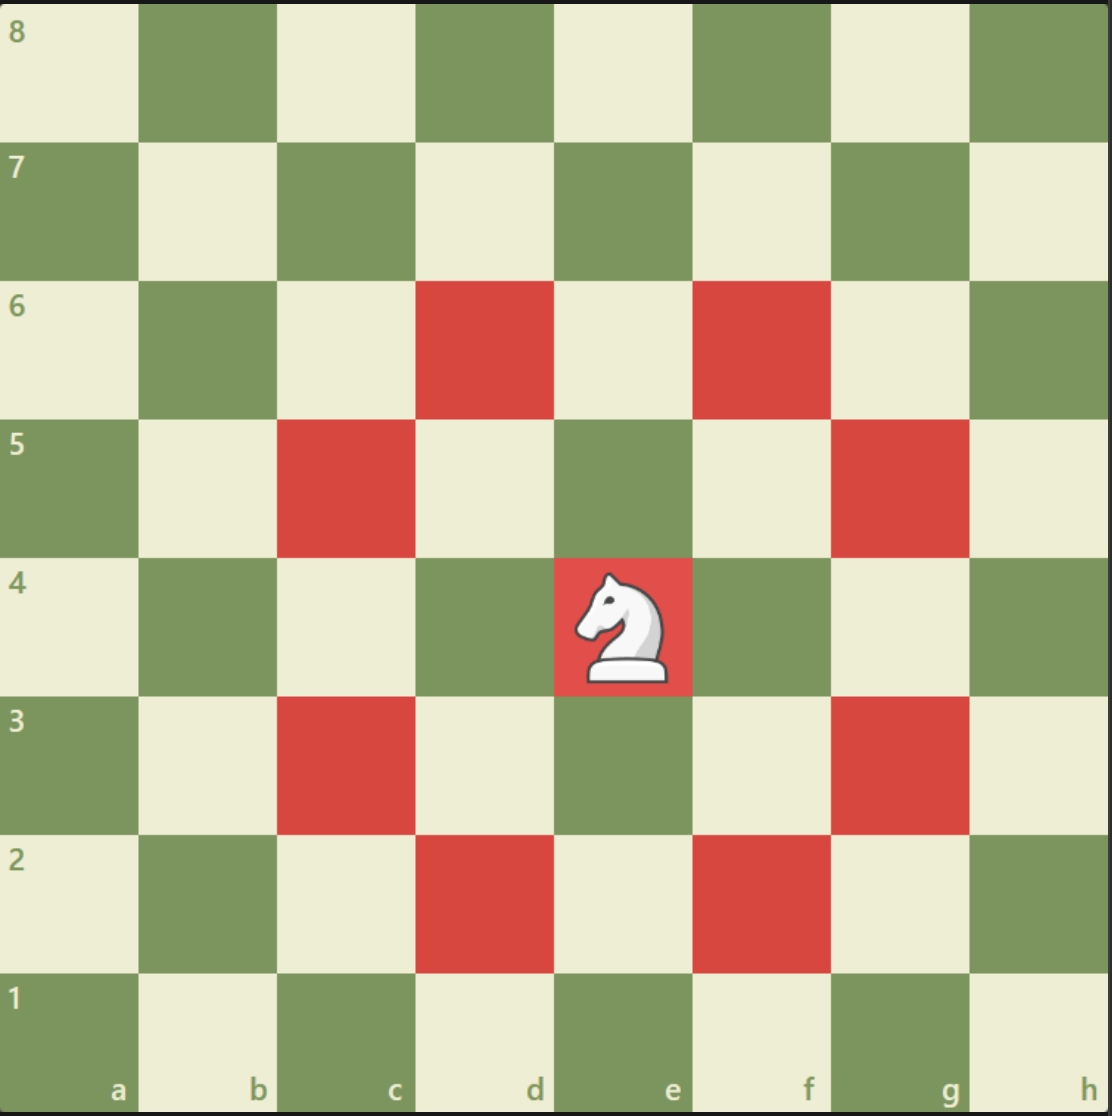
\epsfig{file=Figures/knight-moves.png, scale=0.5}} 
  \caption{The moves of a knight, courtesy of \href{https://www.chess.com/}{chess.com}.}
  \label{fig:knight-moves.png}
\end{figure}

\begin{figure}[!ht]
\centering
\begin{minted}[ frame         = lines, 
                 framesep      = 0.3cm, 
                 firstnumber   = 1,
                 bgcolor       = sepia,
                 numbers       = left,
                 numbersep     = -0.2cm,
                 xleftmargin   = 0.0cm,
                 xrightmargin  = 0.0cm,
               ]{python3}
    import z3
               
    def row(i): return f'R{i}'
    def col(i): return f'C{i}'
    
    def is_knight_move(row, col, rowX, colX):
        Formulas = set()
        for delta_r, delta_c in [(1, 2), (2, 1)]:
            Formulas.add(z3.And(rowX == row + delta_r, colX == col + delta_c))
            Formulas.add(z3.And(rowX == row + delta_r, colX + delta_c == col))
            Formulas.add(z3.And(rowX + delta_r == row, colX == col + delta_c))
            Formulas.add(z3.And(rowX + delta_r == row, colX + delta_c == col)) 
        return z3.Or(*Formulas)
            
    def all_different(Rows, Cols):
        Result = set()
        for i in range(62+1):
            for j in range (i+1, 63+1):
                Result.add(z3.Or(Rows[i] != Rows[j], Cols[i] != Cols[j]))
        return Result
            
    def all_constraints(Rows, Cols):
        Constraints = all_different(Rows, Cols)
        Constraints.add(Rows[0] == 0)
        Constraints.add(Cols[0] == 0)
        for i in range(62+1):
            Constraints.add(is_knight_move(Rows[i], Cols[i], Rows[i+1], Cols[i+1]))
        for i in range(63+1):
            Constraints.add(Rows[i] >= 0) 
            Constraints.add(Cols[i] >= 0) 
        return Constraints
\end{minted}
\vspace*{-0.3cm}
\caption{The Knight's Tour: Computing the constraints.}
\label{fig:Knight's Tour with Z3.ipynb-1}
\end{figure}



Figure \ref{fig:Knight's Tour with Z3.ipynb-1} shows how we can formulate the puzzle using \texttt{Z3}.
\begin{enumerate}
\item In line 1 we import the library \texttt{z3}.
 
\item We define the auxiliary functions \texttt{row} and \texttt{col} in line 3 and 4.
      Given a natural number $i$, the expression $\mathtt{row}(i)$ returns the string $\texttt{'R}i\texttt{'}$
      and  $\mathtt{col}(i)$ returns the string  $\texttt{'C}i\texttt{'}$.  These strings in turn represent the
      variables $\mathtt{R}_i$ and $\mathtt{C}_i$.
\item The function \texttt{is\_knight\_move} takes four parameters:
      \begin{enumerate}
      \item \texttt{row} is a \texttt{Z3} variable that specifies the row of the position of the knight before
            the move. 
      \item \texttt{col} is a \texttt{Z3} variable that specifies the column of the position of the knight
            before the move. 
      \item \texttt{rowX} is a \texttt{Z3} variable that specifies the row of the position of the knight after
            the move. 
      \item \texttt{colX} is a \texttt{Z3} variable that specifies the column of the position of the knight
            after the move. 
      \end{enumerate}
      The function checks whether the move from position 
      $\langle \mathtt{R}_i, \mathtt{C}_i \rangle$ to the position $\langle \mathtt{R}_{i+1}, \mathtt{C}_{i+1} \rangle$
      is a legal move for a knight.  In line 13 we use the fact that the function \texttt{z3.Or}
      can take any number of arguments.  If \texttt{Formulas} is the set 
      \\[0.2cm]
      \hspace*{1.3cm}
      $\texttt{Formulas} = \{f_1, \cdots, f_n\}$,
      \\[0.2cm]
      then the notation \texttt{z3.Or(*Formulas)} is expanded into the call
      \\[0.2cm]
      \hspace*{1.3cm}
      $\texttt{z3.Or}(f_1, \cdots, f_n)$,
      \\[0.2cm]
      which computes the logical disjunction
      \\[0.2cm]
      \hspace*{1.3cm}
      $f_1 \vee \cdots \vee f_n$.
\item The function \texttt{all\_different} takes two parameters:
      \begin{enumerate}[(a)]
      \item \texttt{Rows} is a list of \texttt{Z3} variables. The \texttt{Z3} variable \texttt{Rows[i]}
            specifies the row of the position of the knight after the $i^{\textrm{th}}$ move. 
      \item \texttt{Cols} is a list of \texttt{Z3} variables. The \texttt{Z3} variable \texttt{Cols[i]}
            specifies the column of the position of the knight after the $i^{\textrm{th}}$ move. 
      \end{enumerate}
      The function computes a set of formulas that state that the positions
      $\langle \mathtt{R}_i, \mathtt{C}_i \rangle$ for $i=0,1\cdots, 63$ are all different from each other.
      Note that the position $\langle \mathtt{R}_i, \mathtt{C}_i \rangle$ is different from the position
      $\langle \mathtt{R}_j, \mathtt{C}_j \rangle$ iff $R_i$ is different from $R_j$ or $C_i$ is different from
      $C_j$. 
\item The function \texttt{all\_constraints} computes the set of all constraints.
      The parameters for this function are the same as those for the function \texttt{all\_different}.
      In addition to the constraints already discussed this function specifies that the knight starts
      its tour at the upper left corner of the board.

      Furthermore, there are constraints that the variables $\mathtt{R}_i$ and $\mathtt{C}_i$ are all
      non-negative.  These constraints are needed as we will model the variables with bit vectors of length 4.
      These bit vectors store integers in
      \href{https://en.wikipedia.org/wiki/Two%27s_complement}{two's complement} representation.
      In two's complement representation of a bit vector of length 4 we can model integers from the set
      $\{-8, \cdots, 7\}$.  If we add the number $1$ to a 4-bit bit vector $v$ that represents the number $7$,
      then an overflow will occur and the result will be $-8$ instead of $8$. This could happen in the
      additions that are performed in the formulas computed by the function \texttt{is\_knight\_move}.
      We can exclude these cases by adding the constraints that all variables are non-negative.
\end{enumerate}

\begin{figure}[!ht]
\centering
\begin{minted}[ frame         = lines, 
                 framesep      = 0.3cm, 
                 firstnumber   = 1,
                 bgcolor       = sepia,
                 numbers       = left,
                 numbersep     = -0.2cm,
                 xleftmargin   = 0.8cm,
                 xrightmargin  = 0.8cm,
               ]{python3}
    def solve():
        Rows = [z3.BitVec(row(i), 4) for i in range(63+1)]
        Cols = [z3.BitVec(col(i), 4) for i in range(63+1)]
        Constraints = all_constraints(Rows, Cols)
        S = z3.Solver()
        S.add(Constraints)
        result = str(S.check())
        if result == 'sat':
            Model    = S.model()
            Solution = (  { row(i): Model[Rows[i]] for i in range(63+1) } 
                        | { col(i): Model[Cols[i]] for i in range(63+1) })
            return Solution
        elif result == 'unsat':
            print('The problem is not solvable.')
        else:
            print('Z3 cannot determine whether the problem is solvable.')
\end{minted}
\vspace*{-0.3cm}
\caption{The function \texttt{solve}.}
\label{fig:Knight's Tour with Z3.ipynb-2}
\end{figure}

\begin{figure}[!ht]
  \centering
  \framebox{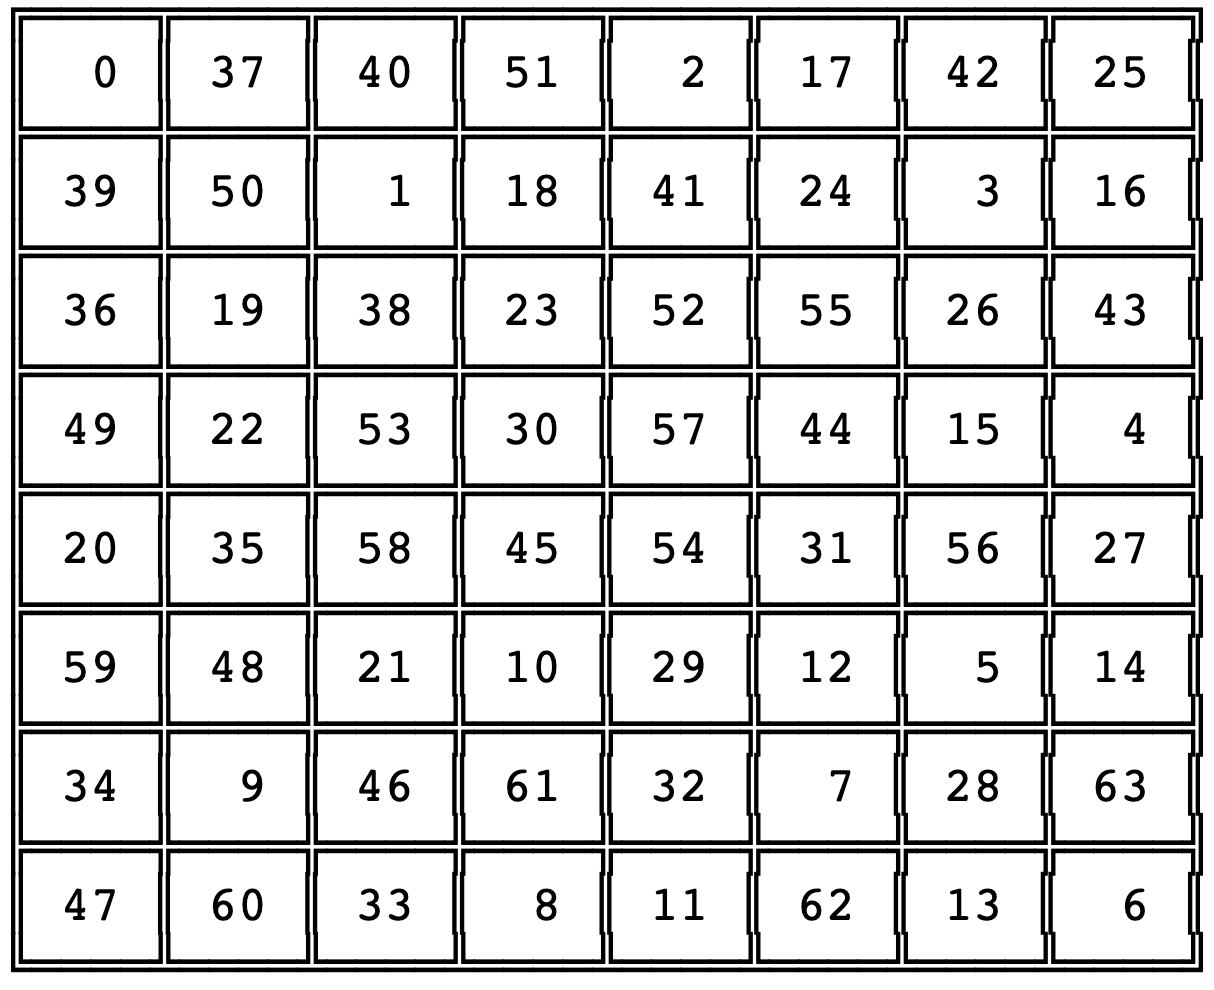
\epsfig{file=Figures/knights-problem.png, scale=0.5}} 
  \caption{A solution of the knight's problem.}
  \label{fig:knights-problem.png}
\end{figure}

Finally, the function \texttt{solve} that is shown in Figure \ref{fig:Knight's Tour with Z3.ipynb-2} on page
\pageref{fig:Knight's Tour with Z3.ipynb-2} can be used to solve the puzzle.
The purpose of the function \texttt{solve} is to construct a \textsc{Csp} encoding the puzzle and to find a
solution of this \textsc{Csp} unsing \texttt{Z3}.
If successful, it returns a dictionary that maps every variable name to the corresponding value of the solution
that has been found.
\begin{enumerate}
\item In line 2 and 3 we create the \texttt{Z3} variables that specify the positions of the knight after its
      $i^{\mathrm{th}}$ move.  $\texttt{Rows}[i]$ specifies the row of the knight after the its
      $i^{\mathrm{th}}$ move, while $\texttt{Cols}[i]$ specifies the column.
\item We compute the set of all constraints in line 4.   
\item We create a solver object in line 5 and add the constraints to this solver in the following line.
\item The function \texttt{check} tries to build a model satisfying the constraints, while the function
      \texttt{model} extracts this model if it exists.
\item Finally, in line 10 and 11 we create a dictionary that maps all of our variables to the corresponding
      values that are found in the model.  Note that $\texttt{row}(i)$ returns the name of the
      \texttt{Z3} variable $\texttt{Rows}[i]$ and similarly $\mathtt{col}(i)$ returns the name of the
      \texttt{Z3} variable $\texttt{Cols}[i]$.
      This dictionary is then returned.
\end{enumerate}
Figure \ref{fig:knights-problem.png} on page \pageref{fig:knights-problem.png} shows a solution that has been
computed by the program discussed above.


\begin{table}[h]
  \centering
  \begin{tabular}{||c|c|c||c|c|c||c|c|c||}
    \hline
    \hline
      & 3 & 9 &   &   &   &   &   & 7 \\
    \hline
      &   &   & 7 &   &   & 4 & 9 & 2 \\
    \hline
      &   &   &   & 6 & 5 &   & 8 & 3 \\
    \hline
    \hline
      &   &   & 6 &   & 3 & 2 & 7 &   \\
    \hline
      &   &   &   & 4 &   & 8 &   &   \\
    \hline
    5 & 6 &   &   &   &   &   &   &   \\
    \hline
    \hline
      &   & 5 & 2 &   & 9 &   &   & 1 \\
    \hline
      & 2 & 1 &   &   &   &   & 4 &   \\
    \hline
    7 &   &   &   &   &   & 5 &   &   \\
    \hline
    \hline
  \end{tabular}
  \caption{A super hard sudoku from the magazine ``Zeit Online''.}
  \label{tab:sudoku}
\end{table}


\exerciseEng
\index{sudoku}
Table \ref{tab:sudoku} on page \pageref{tab:sudoku} shows a \href{https://en.wikipedia.org/wiki/Sudoku}{sudoku}
that I have taken from the
\href{http://sudoku.zeit.de/cgi-bin/sudoku/sudoku_kd_app_2016.pl?action=level&kd_nr=24091123601092&year=2018&month=03&day=23&level=-c+5}{Zeit Online}
magazine.
Solve this sudoku using \texttt{Z3}.  You should start with the following file:
\\[0.2cm]
\hspace*{0.0cm}
\href{https://github.com/karlstroetmann/Logic/blob/master/Python/Chapter-5/Sudoku-Z3.ipynb}{https://github.com/karlstroetmann/Logic/blob/master/Python/Chapter-5/Sudoku-Z3.ipynb}.
    \eox

\section{Normalformen für prädikatenlogische Formeln}
Im nächsten Abschnitt gehen wir daran, einen Kalkül $\vdash$ für die
Prädikaten-Logik zu definieren.  Genau wie im Falle der Aussagen-Logik wird dies wesentlich einfacher, wenn wir
uns auf Formeln beschränken, die in einer \blue{Normalform}  vorliegen.  Bei dieser Normalform handelt es sich
nun um sogenannte \blue{prädikatenlogische Klauseln}.\index{prädikatenlogische Klausel}  Diese werden ähnlich
definiert wie in der 
Aussagen-Logik:  Ein \blue{prädikatenlogisches Literal}\index{prädikatenlogisches Literal} ist eine atomare
Formel oder die Negation einer 
atomaren Formel.  Eine \blue{prädikatenlogische Klausel}\index{prädikatenlogische Klausel} ist dann eine
Disjunktion prädikatenlogischer Literale.  Wir zeigen in diesem Abschnitt, dass jede Formel-Menge $M$
so in eine Menge von prädikatenlogischen Klauseln $K$ transformiert werden kann, dass $M$ genau dann erfüllbar ist, wenn $K$
erfüllbar ist.  Daher ist die Beschränkung auf prädikatenlogische Klauseln keine echte Einschränkung.  Zunächst geben wir einige
Äquivalenzen an, mit deren Hilfe Quantoren manipuliert werden können. 

\begin{Satz}
  Es gelten die folgenden Äquivalenzen:
  \begin{enumerate}
  \item $\models \neg\big(\forall x\colon f\big) \leftrightarrow \big(\exists x\colon \neg f\big)$
  \item $\models \neg\big(\exists x\colon f\big) \leftrightarrow \big(\forall x\colon \neg f\big)$
  \item $\models \forall x\colon f \wedge \forall x\colon g \leftrightarrow \forall x\colon (f \wedge g)$
  \item $\models \exists x\colon f \vee \exists x\colon g \leftrightarrow \exists x\colon (f \vee g)$
  \item $\models \forall x\colon \forall y\colon f \leftrightarrow \forall y\colon  \forall x\colon f$
  \item $\models \exists x\colon \exists y\colon f \leftrightarrow \exists y\colon  \exists x\colon f$
  \item Falls $x$ eine Variable ist, für die $x \not\in \FV(f)$ ist, so haben wir \\[0.2cm]
        \hspace*{1.3cm} $\models  (\forall x\colon f) \leftrightarrow f$ \quad und \quad
                        $\models  (\exists x\colon f) \leftrightarrow f$.
  \item Falls $x$ eine Variable ist, für die  $x \not\in \FV(g)$ gilt, so haben wir die folgenden Äquivalenzen:
    \begin{enumerate}
    \item $\models (\forall x\colon f) \vee g \leftrightarrow \forall x\colon (f \vee g)$ \quad und \quad $\models g \vee (\forall x\colon f) \leftrightarrow \forall x\colon (g \vee f)$,
    \item $\models (\exists x\colon f) \wedge g \leftrightarrow \exists x\colon (f \wedge g)$ \quad und \quad $\models g \wedge (\exists x\colon f) \leftrightarrow \exists x\colon (g \wedge f)$.
    \end{enumerate}
  \end{enumerate}
\end{Satz}

Um die Äquivalenzen der letzten Gruppe anwenden zu können, kann es notwendig sein,
gebundene Variablen umzubenennen. Ist $f$ eine prädikatenlogische Formel und sind $x$ und
$y$ zwei Variablen, wobei $y$ nicht in $f$ auftritt, so bezeichnet \blue{$f[x/y]$} die Formel, die aus $f$
dadurch entsteht, dass jedes Auftreten der Variablen $x$ in $f$ durch $y$ ersetzt wird.  Beispielsweise gilt \\[0.2cm]
\hspace*{1.3cm} $\bigl(\forall u : \exists v : p(u,v)\bigr)[u/z] = \forall z : \exists v : p(z,v)$
\\[0.2cm]
Damit können wir eine letzte Äquivalenz angeben: Ist $f$ eine prädikatenlogische Formel,
ist $x \in BV(f)$ und ist $y$ eine Variable, die in $f$ nicht auftritt, so gilt \\[0.2cm]
\hspace*{1.3cm} $\models f \leftrightarrow f[x/y]$.
\vspace{0.3cm}

Mit Hilfe der oben stehenden Äquivalenzen und der aussagenlogischen Äquivalenzen, die wir schon kennen, können
wir eine Formel so umformen, dass die Quantoren nur noch außen stehen.  Eine solche Formel ist dann in
\blue{pränexer Normalform}.\index{pränexer Normalform}  Wir führen das Verfahren an einem Beispiel vor: Wir
zeigen, dass die Formel  
\\[0.2cm]
\hspace*{1.3cm}
$\bigl(\forall x\colon p(x)\bigr) \rightarrow \bigl(\exists x\colon p(x)\bigr)$ 
\\[0.2cm]
allgemeingültig ist: 
$$ 
\begin{array}{ll}
                 & \bigl(\forall x\colon p(x)\bigr) \rightarrow \bigl(\exists x\colon p(x)\bigr)  \\
 \Leftrightarrow & \neg \bigl(\forall x\colon p(x)\bigr) \vee \bigl(\exists x\colon p(x)\bigr)    \\
 \Leftrightarrow & \bigl(\exists x\colon \neg p(x)\bigr) \vee \bigl(\exists x\colon p(x)\bigr)    \\
 \Leftrightarrow & \exists x\colon \bigl(\neg p(x) \vee p(x)\bigr) \\
 \Leftrightarrow & \exists x\colon \verum                                                  \\
 \Leftrightarrow & \verum                                                  \\
\end{array}
$$
\\[0.2cm]
In diesem Fall haben wir Glück gehabt, dass es uns gelungen ist, die Formel als Tautologie zu
erkennen.  Im Allgemeinen reichen die obigen Umformungen aber nicht aus, um prädikatenlogische
Tautologien erkennen zu können.  Um Formeln noch stärker vereinfachen zu können, 
führen wir einen weiteren Äquivalenz-Begriff ein.  Diesen Begriff wollen wir vorher durch ein Beispiel
motivieren.  Wir betrachten die beiden Formeln 
\\[0.2cm]
\hspace*{1.3cm} $f_1 = \forall x \colon \exists y \colon p(x,y)$ \quad und \quad $f_2 = \forall x \colon
p\bigl(x,s(x)\bigr)$.
\\[0.2cm]
Die beiden Formeln $f_1$ und $f_2$ sind nicht äquivalent, denn sie entstammen noch nicht
einmal der gleichen Signatur: In der Formel $f_2$ wird das Funktions-Zeichen $s$
verwendet, das in der Formel $f_1$ überhaupt nicht auftritt. 
Auch wenn die beiden Formeln $f_1$ und $f_2$ nicht äquivalent sind, so besteht zwischen
ihnen doch die folgende Beziehung:  Ist $\textsl{S}_1$ eine
prädikatenlogische Struktur, in der die Formel $f_1$ gilt:
\\[0.2cm]
\hspace*{1.3cm}
$\mathcal{S}_1 \models f_1$,
\\[0.2cm]
dann können wir diese Struktur zu einer Struktur $\textsl{S}_2$ erweitern, in der die
Formel $f_2$ gilt:
\\[0.2cm]
\hspace*{1.3cm}
$\mathcal{S}_2 \models f_2$.
\\[0.2cm]
Dazu muss die Interpretation des Funktions-Zeichens $s$ so gewählt werden, dass
für jedes $x$ tatsächlich $p\bigl(x,s(x)\bigr)$ gilt.  Dies ist möglich, denn die Formel $f_1$ sagt ja aus, 
dass wir zu jedem $x$ einen Wert $y$ finden, für den $p(x,y)$ gilt.   Die Funktion $s$ muss also lediglich zu 
jedem $x$ dieses $y$ zurück geben. 



\begin{Definition}[{\color{blue}Skolemisierung}]\index{Skolemisierung} \hspace*{\fill} \linebreak
  Es sei $\Sigma = \langle \mathcal{V}, \mathcal{F}, \mathcal{P}, \textsl{arity} \rangle$
  eine Signatur.  Ferner sei $f$ eine geschlossene $\Sigma$-Formel der Form \\[0.2cm]
  \hspace*{1.3cm} 
  $f = \forall x_1, \cdots, x_n \colon \exists y \colon g$. \\[0.2cm]
  Dann wählen wir ein \underline{\blue{neues}} $n$-stelliges Funktions-Zeichen $s$, d.h.~wir nehmen ein Zeichen $s$, dass in
  der Signatur $\Sigma$ nicht auftritt und erweitern die Signatur $\Sigma$ zu der Signatur \\[0.2cm]
  \hspace*{1.3cm} 
  $\Sigma' := \Bigl\langle \mathcal{V}, \mathcal{F} \cup \{s\}, \mathcal{P}, \textsl{arity} \cup \bigl\{\pair(s,n)\bigr\} \Bigr\rangle$, \\[0.2cm]
  in der wir $s$ als neues $n$-stelliges Funktions-Zeichen deklarieren.  Anschließend definieren wir die $\Sigma'$-Formel
  $f'$ wie folgt: \\[0.2cm]
  \hspace*{1.3cm} 
  $f' := \mathtt{Skolem}(f) := 
  \forall x_1 \colon \cdots \forall x_n \colon g\bigl[y \mapsto s(x_1,\cdots,x_n)\bigr]$
  \\[0.2cm]
  Hierbei bezeichnet der Ausdruck $g\bigl[y \mapsto s(x_1,\cdots,x_n)\bigr]$ die Formel, die wir aus $g$
  dadurch erhalten, dass wir jedes Auftreten der Variablen $y$ in der Formel $g$ durch den Term
  $s(x_1,\cdots,x_n)$ ersetzen.  Wir sagen, dass die Formel $f'$ aus der Formel $f$
  durch einen \blue{Skolemisierungs-Schritt} hervorgegangen ist. 
  \eox
\end{Definition}
\vspace{-0.5cm}

\example
Es $f$ die folgende Formel aus der Gruppen-Theorie:
\\[0.2cm]
\hspace*{1.3cm}
$f := \forall x: \exists y: y * x = 1$. 
\\[0.2cm]
Dann gilt
\\[0.2cm]
\hspace*{1.3cm}
$\mathtt{Skolem}(f) = \forall x : s(x) * x = 1$.  \eox

\noindent
In welchem Sinne sind eine Formel $f$ und eine Formel $f'$, die aus $f$ durch einen 
Skolem\-isierungs-Schritt hervorgegangen sind, äquivalent?  Zur Beantwortung dieser Frage
dient die folgende Definition. 

\begin{Definition}[Erfüllbarkeits-Äquivalenz] \hspace*{\fill} \linebreak
   Zwei geschlossene Formeln $f$ und $g$ heißen 
   \blue{erfüllbarkeits-äquivalent}\index{erfüllbarkeits-äquivalent}
   falls $f$ und $g$ entweder beide erfüllbar oder beide unerfüllbar sind.
   Wenn $f$ und $g$ erfüllbarkeits-äquivalent sind, so schreiben wir \\[0.2cm]
   \hspace*{1.3cm} $f \approx_e g$.
\eox
\end{Definition}

\noindent
\textbf{Beobachtung:}
Falls die Formel $f'$ aus der Formel $f$ durch einen Skolemisierungs-Schritt 
hervorgegangen ist, so sind $f$ und $f'$ erfüllbarkeits-äquivalent, denn wir können jede Struktur
$\mathcal{S}$, in der die Formel $f$ gilt, zu einer Struktur $\mathcal{S}'$ erweitern, in der auch $f'$ gilt.
\eox

Wir können nun ein einfaches Verfahren angeben, um Existenz-Quantoren aus einer Formel
zu eliminieren.  Dieses Verfahren besteht aus zwei Schritten:  Zunächst bringen wir die Formel
in pränexe Normalform. Anschließend können wir die Existenz-Quantoren der Reihe nach durch \linebreak
Skolemisierungs-Schritte eliminieren.  Nach dem oben gemachten Bemerkungen ist die resultierende 
Formel zu der ursprünglichen Formel erfüllbarkeits-äquivalent.  Dieses
Verfahren der Eliminierung von Existenz-Quantoren durch die Einführung neuer
Funktions-Zeichen wird als \blue{Skolemisierung} bezeichnet.  Haben wir eine Formel $F$
in pränexe Normalform gebracht und anschließend skolemisiert, so hat das Ergebnis die Gestalt\\[0.2cm]
\hspace*{1.3cm} $\forall x_1, \cdots, x_n: g$ \\[0.2cm]
und in der Formel $g$ treten keine Quantoren mehr auf.  Die Formel $g$ wird auch als die
\blue{Matrix}\index{Matrix} der obigen Formel bezeichnet.  Wir können nun  $g$ mit Hilfe
der uns aus dem letzten Kapitel bekannten aussagenlogischen
 Äquivalenzen in konjunktive Normalform bringen.  Wir haben dann eine
Formel der Gestalt \\[0.2cm]
\hspace*{1.3cm} $\forall x_1, \cdots, x_n: (k_1 \wedge \cdots \wedge k_m)$. \\[0.2cm]
Dabei sind die $k_i$ Disjunktionen von prädikatenlogischen \blue{Literalen}.  Wenden wir
hier  die Äquivalenz 
\\[0.2cm]
\hspace*{1.3cm}
$\forall x\colon (f_1\wedge f_2) \leftrightarrow (\forall x\colon f_1) \wedge (\forall x\colon f_2)$
\\[0.2cm]
an, so können wir die All-Quantoren auf die einzelnen $k_i$ verteilen und
die resultierende Formel hat die Gestalt \\[0.2cm]
\hspace*{1.3cm} 
$\big(\forall x_1, \cdots, x_n: k_1\big) \wedge \cdots \wedge \big(\forall x_1, \cdots, x_n: k_m\big)$. \\[0.2cm]
Ist eine Formel $F$ in der obigen
Gestalt, so sagen wir, dass $F$ in \blue{prädikatenlogischer Klausel-Normalform}
\index{prädikatenlogische Klausel-Normalform}  ist und eine Formel der Gestalt \\[0.2cm]
\hspace*{1.3cm} $\forall x_1, \cdots, x_n: k$, \\[0.2cm]
bei der $k$ eine Disjunktion prädikatenlogischer Literale ist,
bezeichnen wir als \blue{prädikatenlogische Klausel}.  \index{prädikatenlogische Klausel} Ist $M$
eine Menge von Formeln deren Erfüllbarkeit wir untersuchen wollen, so können wir nach dem
bisher Gezeigten  $M$ immer in eine erfüllbarkeits-äquivalente Menge prädikatenlogischer Klauseln umformen.
Da  dann nur noch All-Quantoren vorkommen, können wir hier die  Notation noch vereinfachen,
indem wir vereinbaren, dass alle Formeln implizit allquantifiziert sind, wir lassen also
die All-Quantoren weg.

\noindent
Das Jupyter Notebook
\\[0.2cm]
\hspace*{0.8cm}
\href{https://github.com/karlstroetmann/Logic/blob/master/Python/Chapter-5/FOL-CNF.ipynb}{https://github.com/karlstroetmann/Logic/blob/master/Python/Chapter-5/FOL-CNF.ipynb}.
\\[0.2cm]
enthält ein \textsl{Python}-Programm, mit dessen Hilfe wir prädikatenlogische Formeln in eine \linebreak
erfüllbarkeits-äquivalente Menge von prädikatenlogischen Klauseln umformen können.

Wozu sind nun die Umformungen in Skolem-Normalform gut?  Es geht darum, dass wir 
ein Verfahren entwickeln wollen, mit dem es möglich ist für eine prädikatenlogische Formel
$f$ zu zeigen, dass $f$ allgemeingültig ist, dass also \\[0.2cm]
\hspace*{1.3cm} $\models f$ \\[0.2cm]
gilt.  Wir wissen, dass \\[0.2cm]
\hspace*{1.3cm} $\models f$ \quad g.d.w. \quad $\{\neg f\} \models \falsum$ \\[0.2cm]
gilt, denn die Formel $f$ ist genau dann allgemeingültig, wenn es keine Struktur gibt, in
der die Formel $\neg f$ erfüllbar ist. 
 Wir bilden daher zunächst die Formel $\neg f$ und formen dann diese Formel in prädikatenlogische
Klausel-Normalform um.  Wir erhalten Klauseln $k_1, \cdots, k_n$, so dass  \\[0.2cm]
\hspace*{1.3cm} $\neg f \approx_e k_1 \wedge \cdots \wedge k_n$ \\[0.2cm]
gilt.  Anschließend versuchen wir,
aus den Klauseln $k_1,\cdots,k_n$ einen Widerspruch herzuleiten: \\[0.2cm]
\hspace*{1.3cm} $\{k_1, \cdots, k_n\} \vdash \falsum$ \\[0.2cm]
Wenn dies gelingt, dann wissen wir, dass die Menge $\{k_1, \cdots, k_n\}$ unerfüllbar ist.
Damit ist auch $\neg f$ unerfüllbar und also ist $f$ allgemeingültig.
Damit wir aus den Klauseln $k_1,\cdots,k_n$ einen Widerspruch herleiten können,
brauchen wir natürlich noch einen Kalkül $\vdash$, der mit prädikatenlogischen Klauseln arbeitet. 
Einen solchen Kalkül werden wir im übernächsten Abschnitt vorstellen.

Um das Verfahren näher zu erläutern demonstrieren wir es an einem Beispiel. 
Wir wollen untersuchen, ob \\[0.2cm]
\hspace*{1.3cm} 
$\models \big(\exists x\colon \forall y\colon  p(x,y)\big) \rightarrow \big(\forall y\colon \exists x\colon p(x,y)\big)$ \\[0.2cm]
gilt.  Wir wissen, dass dies äquivalent dazu ist, dass  \\[0.2cm]
\hspace*{1.3cm} 
$\Big\{ \neg \Big(\big(\exists x\colon \forall y\colon  p(x,y)\big) \rightarrow  \big(\forall y\colon \exists x\colon p(x,y)\big)\Big)\Big\} \models \falsum$ \\[0.2cm]
gilt.  Wir bringen zunächst die negierte Formel in pränexe Normalform. 
$$
\begin{array}{ll}
                  & \neg \Big(\big(\exists x\colon \forall y\colon  p(x,y)\big) \rightarrow \big(\forall y\colon \exists x\colon p(x,y)\big)\Big) \\
  \leftrightarrow & \neg \Big(\neg \big(\exists x\colon \forall y\colon  p(x,y)\big) \vee \big(\forall y\colon \exists x\colon p(x,y)\big)\Big) \\
  \leftrightarrow &                \big(\exists x\colon \forall y\colon  p(x,y)\big) \wedge \neg \big(\forall y\colon \exists x\colon p(x,y)\big) \\
  \leftrightarrow &\big(\exists x\colon \forall y\colon  p(x,y)\big) \wedge  \big(\exists y\colon  \neg \exists x\colon p(x,y)\big) \\
  \leftrightarrow &\big(\exists x\colon \forall y\colon  p(x,y)\big) \wedge  \big(\exists y\colon  \forall x\colon \neg p(x,y)\big) \\
\end{array}
$$
Um an dieser Stelle weitermachen zu können, ist es nötig, die Variablen in dem  zweiten
Glied der Konjunktion umzubenennen.  Wir ersetzen $x$ durch $u$ und $y$ durch $v$ und erhalten
$$
\begin{array}{ll}
                  &\big(\exists x\colon \forall y\colon  p(x,y)\big) \wedge  \big(\exists y\colon  \forall x\colon \neg p(x,y)\big) \\
  \leftrightarrow &\big(\exists x\colon \forall y\colon  p(x,y)\big) \wedge  \big(\exists v\colon  \forall u\colon \neg p(u,v)\big) \\
  \leftrightarrow &\exists v\colon  \Big( \big(\exists x\colon \forall y\colon  p(x,y)\big) \wedge  \big(\forall u\colon \neg p(u,v)\big) \Big)\\
  \leftrightarrow &\exists v\colon  \exists x\colon  \Big( \big(\forall y\colon  p(x,y)\big) \wedge \big(\forall u\colon \neg p(u,v)\big) \Big)\\
  \leftrightarrow &\exists v\colon  \exists x\colon \forall y\colon \Big( p(x,y) \wedge \big(\forall u\colon \neg p(u,v)\big) \Big)\\
  \leftrightarrow &\exists v\colon  \exists x\colon \forall y\colon \forall u\colon \Big( p(x,y) \wedge \neg p(u,v) \Big)\\
\end{array}
$$
An dieser Stelle müssen wir skolemisieren um die Existenz-Quantoren los zu werden. 
Wir führen dazu zwei neue Funktions-Zeichen $s_1$ und $s_2$ ein. 
Dabei gilt $\mathtt{arity}(s_1) = 0$ und $\mathtt{arity}(s_2) = 0$, denn vor den
Existenz-Quantoren stehen keine All-Quantoren.
$$
\begin{array}{ll}
           & \exists v\colon  \exists x\colon \forall y\colon \forall u\colon \Big( p(x,y) \wedge \neg p(u,v) \Big)\\
 \approx_e & \exists x\colon \forall y\colon \forall u\colon \Big( p(x,y) \wedge \neg p(u,s_1) \Big)\\
 \approx_e & \forall y\colon \forall u\colon \Big( p(s_2,y) \wedge \neg p(u,s_1) \Big)\\
\end{array}
$$
Da jetzt nur noch All-Quantoren auftreten, können wir diese auch noch weglassen,
da wir ja ver\-einbart haben, dass alle freien Variablen implizit allquantifiziert sind.
Damit können wir nun die prädikatenlogische Klausel-Normalform in Mengen-Schreibweise angeben, diese
ist
\\[0.2cm] 
\hspace*{1.3cm}
$M := \Big\{ \big\{ p(s_2,y) \big\}, \big\{\neg p(u,s_1)\big\}\Big\}$.
\\[0.2cm]
Wir zeigen, dass die Menge $M$ widersprüchlich ist.
Dazu betrachten wir zunächst die Klausel $\big\{ p(s_2,y) \big\}$ und setzen in
dieser Klausel für $y$ die Konstante $s_1$ ein.  Damit erhalten wir die Klausel \\[0.2cm]
\hspace*{1.3cm}  $\big\{ p(s_2,s_1) \big\}$. \hspace*{\fill}(1)\\[0.2cm]
Das Ersetzung von $y$ durch $s_1$ begründen wir damit, dass die obige Klausel ja implizit
allquantifiziert ist und wenn etwas für alle $y$ gilt, dann sicher auch für $y = s_1$.

Als nächstes betrachten wir die Klausel $\big\{\neg p(u,s_1)\big\}$.
Hier setzen wir für die Variablen $u$ die Konstante $s_2$ ein und erhalten dann die
Klausel \\[0.2cm]
\hspace*{1.3cm} $\big\{\neg p(s_2,s_1)\big\}$ \hspace*{\fill} (2) \\[0.2cm]
Nun wenden wir auf die Klauseln (1) und (2) die Schnitt-Regel an und finden \\[0.2cm]
\hspace*{1.3cm} 
$\big\{ p(s_2,s_1) \big\}$, \quad$\big\{\neg p(s_2,s_1)\big\}$ \quad $\vdash \quad \{\}$.
\\[0.2cm]
Damit haben wir einen Widerspruch hergeleitet und gezeigt, dass die Menge $M$ unerfüllbar
ist. Damit ist dann auch \\[0.2cm]
\hspace*{1.3cm} 
$\Big\{ \neg \Big(\big(\exists x\colon \forall y\colon  p(x,y)\big) \rightarrow  \big(\forall y\colon \exists x\colon p(x,y)\big)\Big)\Big\}$
\\[0.2cm]
unerfüllbar und folglich gilt \\[0.2cm]
\hspace*{1.3cm} 
$\models \big(\exists x\colon \forall y\colon  p(x,y)\big) \rightarrow  \big(\forall y\colon \exists x\colon p(x,y)\big)$.

\section{Unifikation}
In dem  Beispiel im letzten Abschnitt haben wir die Terme $s_1$ und $s_2$ geraten, die wir für die Variablen
$y$ und $u$ in den Klauseln $\big\{ p(s_2,y) \big\}$ und  $\big\{\neg p(u,s_1)\big\}$
eingesetzt haben.  Wir haben diese Terme mit dem Ziel gewählt, später die Schnitt-Regel
anwenden zu können.  In diesem Abschnitt zeigen wir nun ein Verfahren, mit dessen Hilfe
wir die benötigten Terme ausrechnen können.
Dazu benötigen wir zunächst den Begriff einer \blue{Substitution}.
\begin{Definition}[Substitution]\index{Substitution}
    Es sei eine Signatur \\[0.2cm]
    \hspace*{1.3cm} $\Sigma = \langle \mathcal{V}, \mathcal{F}, \mathcal{P}, \textsl{arity} \rangle$ \\[0.2cm]
    gegeben.  Eine {\color{blue}$\Sigma$-Substitution} ist eine endliche Menge von Paaren der Form \\[0.2cm]
    \hspace*{1.3cm} $\sigma = \bigl\{ \langle x_1, t_1 \rangle, \cdots, \langle x_n, t_n \rangle \bigr\}$. \\[0.2cm]
    Dabei gilt:
    \begin{enumerate}
    \item $x_i \in \mathcal{V}$, die $x_i$ sind also Variablen.
    \item $t_i \in \mathcal{T}_\Sigma$, die $t_i$ sind also Terme.
    \item Für $i\not=j$ ist $x_i \not= x_j$, die Variablen sind also paarweise verschieden.
    \end{enumerate}
    
    Ist $\sigma = \bigl\{ \langle x_1, t_1 \rangle, \cdots, \langle x_n, t_n \rangle \bigr\}$ eine
    $\Sigma$-Substitution, so schreiben wir  \\[0.2cm]
    \hspace*{1.3cm} $\sigma = \bigl[ x_1 \mapsto t_1, \cdots, x_n \mapsto t_n \bigr]$.  \\[0.2cm]
    Außerdem definieren wir den \blue{Domain} einer Substitution als \\[0.2cm]
    \hspace*{1.3cm} $\textsl{dom}(\sigma) := \{ x_1, \cdots, x_n\}$.
    \\[0.2cm]
    Die Menge aller Substitutionen bezeichnen wir mit \blue{\textsl{Subst}}.\index{Subst}
    \eox
\end{Definition}

\noindent
Substitutionen werden für uns dadurch interessant, dass wir sie auf Terme \blue{anwenden} können.  Ist $t$ ein
Term und $\sigma$ eine Substitution, so ist $t\sigma$ der Term, der aus $t$ dadurch entsteht, dass jedes
Vorkommen einer Variablen $x_i$ durch den zugehörigen Term $t_i$ ersetzt wird.  Die formale Definition folgt. 
\begin{Definition}[Anwendung einer Substitution]
\hspace*{\fill} \\
Es sei $t$ ein Term und es sei $\sigma = \bigl[ x_1 \mapsto t_1, \cdots, x_n \mapsto t_n \bigr]$
eine Substitution. Wir definieren die \blue{Anwendung}\index{Anwending einer Substitution} von $\sigma$ auf $t$
(Schreibweise \blue{$t\sigma$}) \index{$t\sigma$} durch Induktion über 
den Aufbau von $t$: 
\begin{enumerate}
\item Falls $t$ eine Variable ist, gibt es zwei Fälle:
  \begin{enumerate}
  \item $t = x_i$ für ein $i\in\{1,\cdots,n\}$.  Dann definieren wir \quad  $x_i\sigma := t_i$.
  \item $t = y$ mit $y\in\mathcal{V}$, aber $y \not\in \{x_1,\cdots,x_n\}$. Dann definieren wir \quad $y\sigma := y$.
  \end{enumerate}
\item Andernfalls muss $t$ die Form $t= f(s_1,\cdots,s_m)$ haben. Dann können wir $t\sigma$ durch \\[0.2cm]
      \hspace*{1.3cm} $f(s_1, \cdots, s_m)\sigma := f(s_1\sigma, \cdots, s_m\sigma)$. \\[0.2cm]
      definieren, denn nach Induktions-Voraussetzung sind die Ausdrücke $s_i\sigma$ bereits definiert.      
      \eox
\end{enumerate}
\end{Definition}

Genau wie wir Substitutionen auf Terme anwenden können, können wir eine Substitution
auch auf prädikatenlogische Klauseln anwenden.  Dabei werden Prädikats-Zeichen und
Junktoren wie Funktions-Zeichen behandelt.
Wir ersparen uns eine formale Definition und geben stattdessen zunächst einige Beispiele. 
Wir definieren eine Substitution $\sigma$ durch \\[0.2cm]
\hspace*{1.3cm} $\sigma := \big[ x_1 \mapsto c,\; x_2 \mapsto f(d) \big]$. \\[0.2cm]
In den folgenden drei Beispielen demonstrieren wir zunächst, wie eine Substitution
auf einen Term angewendet werden kann.  Im vierten Beispiel wenden wir die Substitution
dann auf eine Klausel in Mengen-Schreibweise an:
\begin{enumerate}
\item $x_3\sigma = x_3$,
\item $f(x_2)\sigma = f\bigl(f(d)\bigr)$,
\item $h(x_1,g(x_2))\sigma = h\bigl(c,g(f(d))\bigr)$.
\item $\bigl\{ p(x_2), q(d,h(x_3,x_1))\bigr\}\sigma = \bigl\{ p(f(d)),\; q(d,h(x_3,c))\bigr\}$.
\end{enumerate}


\noindent
Als nächstes zeigen wir, wie  Substitutionen miteinander verknüpft werden können.
\begin{Definition}[Komposition von Substitutionen] \index{Komposition von Substitutionen}
    Es seien\\[0.2cm]
    \hspace*{1.3cm}  $\sigma = \big[ x_1 \mapsto s_1, \cdots, x_m \mapsto s_m \big]$ \quad und \quad  $\tau = \big[ y_1 \mapsto t_1, \cdots, y_n \mapsto t_n \big]$ \\[0.2cm]
    zwei Substitutionen mit $\textsl{dom}(\sigma) \cap \textsl{dom}(\tau) = \{\}$. Dann definieren
    wir die \blue{Komposition von Substitutionen} $\sigma\tau$ \index{$\sigma\tau$} von $\sigma$ und $\tau$ als \\[0.2cm]
    \hspace*{1.3cm} $\sigma\tau := \big[ x_1 \mapsto s_1\tau, \cdots, x_m \mapsto s_m\tau,\; y_1 \mapsto t_1, \cdots, y_n \mapsto t_n \big]$
    \eox
\end{Definition}

\example
Wir führen das obige Beispiel fort und setzen \\[0.2cm]
\hspace*{1.3cm} $\sigma := \big[ x_1 \mapsto c,\; x_2 \mapsto f(x_3) \big]$
                \quad und \quad $\tau := \big[ x_3 \mapsto h(c,c),\; x_4 \mapsto d \big]$. \\[0.2cm]
Dann gilt: \\[0.2cm]
\hspace*{1.3cm} $ \sigma\tau = \big[ x_1 \mapsto c,\; x_2 \mapsto f(h(c,c)),\; x_3 \mapsto h(c,c),\;x_4 \mapsto d \big]$.
\hspace*{\fill} $\Box$
\vspace{0.3cm}

\noindent
Die Definition der Komposition von Substitutionen ist mit dem Ziel gewählt worden, dass
der folgende Satz gilt.
\begin{Satz} \label{satz:komposition}
    Ist $t$ ein Term und sind $\sigma$ und $\tau$ Substitutionen mit 
    $\textsl{dom}(\sigma) \cap \textsl{dom}(\tau) = \{\}$, so gilt \\[0.2cm]
    \hspace*{1.3cm} $(t \sigma)\tau = t (\sigma\tau)$.
    \hspace*{\fill} $\Box$
\end{Satz}
Der Satz kann durch Induktion über den Aufbau des Termes $t$ bewiesen werden.


\begin{Definition}[Syntaktische Gleichung] \index{syntaktische Gleichung}
Unter einer \blue{syntaktischen Gleichung} verstehen wir in diesem Abschnitt ein Konstrukt der Form
$s \doteq t$, \index{$s \doteq t$} wobei einer der beiden folgenden Fälle vorliegen muss:
\begin{enumerate}
\item $s$ und $t$ sind Terme  oder
\item $s$ und $t$ sind atomare Formeln.
\end{enumerate}
Weiter definieren wir ein \blue{syntaktisches Gleichungs-System} als eine Menge
von syntaktischen Glei\-chun\-gen. \index{syntaktisches Gleichungs-System}
\eox
\end{Definition}

Was syntaktische Gleichungen angeht, so machen wir keinen Unterschied zwischen Funktions-Zeichen und
Prädikats-Zeichen.   Dieser Ansatz ist deswegen berechtigt, weil wir Prädikate
ja auch als spezielle Funktionen auffassen können, nämlich als solche
Funktionen, die als Ergebnis einen Wahrheitswert aus der Menge  $\mathbb{B}$ zurück geben.

\begin{Definition}[Unifikator]
Eine Substitution $\sigma$ \blue{löst} \index{Lösung einer syntaktischen Gleichungen} eine syntaktische
Gleichung $s \doteq t$ genau dann, wenn 
$s\sigma = t\sigma$ ist, wenn also durch die Anwendung von $\sigma$ auf $s$ und $t$
tatsächlich identische Objekte entstehen.  Ist $E$ ein syntaktisches Gleichungs-System, so 
sagen wir, dass $\sigma$ ein \blue{Unifikator} \index{Unifikator} von $E$ ist wenn $\sigma$ jede
syntaktische Gleichung in $E$ löst. 
\eox
\end{Definition}
Ist $E = \{ s_1 \doteq t_1, \cdots, s_n \doteq t_n \}$ eine syntaktisches Gleichungs-System
und ist $\sigma$ eine Substitution, so definieren wir \\[0.2cm]
\hspace*{1.3cm}  $E\sigma := \{ s_1\sigma \doteq t_1\sigma, \cdots, s_n\sigma \doteq t_n\sigma \}$.
\vspace{0.3cm}

\example
Wir verdeutlichen die bisher eingeführten Begriffe anhand eines Beispiels.  
Wir betrachten die Gleichung \\[0.2cm]
\hspace*{1.3cm} $p(x_1, f(x_4)) \doteq p( x_2, x_3)$ \\[0.2cm]
und definieren die Substitution \\[0.2cm]
\hspace*{1.3cm} $\sigma := \big[ x_1 \mapsto x_2,\; x_3 \mapsto f(x_4) \big]$. \\[0.2cm]
Die Substitution $\sigma$ löst die obige syntaktische Gleichung, denn es gilt \\[0.2cm]
\hspace*{1.3cm} $p(x_1, f(x_4))\sigma = p(x_2, f(x_4))$ \quad und \quad \\[0.2cm]
\hspace*{1.3cm} $p(x_2, x_3)\sigma \;\quad = p(x_2, f(x_4))$.  \eox


Als nächstes entwickeln wir ein Verfahren, mit dessen Hilfe wir von einer vorgegebenen
Menge $E$ von syntaktischen Gleichungen entscheiden können, ob es einen Unifikator $\sigma$ für $E$
gibt.  Das Verfahren, das wir entwickeln werden, wurde von Martelli und Montanari veröffentlicht
\cite{martelli:1982}.\index{Verfahren von Martelli und Montanari}  
Wir überlegen uns zunächst, in welchen Fällen wir eine syntaktischen Gleichung $s \doteq t$
garantiert nicht lösen können.  Da gibt es zwei Möglichkeiten: Eine syntaktische Gleichung  \\[0.2cm]
\hspace*{1.3cm} $f(s_1,\cdots,s_m) \doteq g(t_1,\cdots, t_n)$ \\[0.2cm]
ist sicher dann nicht durch eine Substitution lösbar, wenn $f$ und $g$ verschiedene
Funktions-Zeichen sind, denn für jede Substitution $\sigma$ gilt ja \\[0.2cm]
\hspace*{1.0cm} $f(s_1,\cdots,s_m)\sigma = f(s_1\sigma,\cdots,s_m\sigma)$ \quad und \quad
                $g(t_1,\cdots, t_n)\sigma = g(t_1\sigma,\cdots,t_n\sigma)$. \\[0.2cm]
Falls $f \not = g$ ist, haben die Terme  $f(s_1,\cdots,s_m)\sigma$ und $g(t_1,\cdots, t_n)\sigma$ verschieden
Funktions-Zeichen und können daher syntaktisch nicht identisch werden.

Die andere Form einer syntaktischen Gleichung, die garantiert unlösbar ist, ist\\[0.2cm]
\hspace*{1.3cm} $x \doteq f(t_1,\cdots,t_n)$  \quad falls $x \in \textsl{Var}\big(f(t_1,\cdots,t_n)\big)$. \\[0.2cm]
Das diese syntaktische Gleichung unlösbar ist liegt daran, dass die rechte Seite immer mindestens ein
Funktions-Zeichen mehr enthält als die linke.  

Mit diesen Vorbemerkungen können wir nun ein Verfahren angeben, mit dessen Hilfe es
möglich ist, Mengen von syntaktischen Gleichungen zu lösen, oder festzustellen, dass es
keine Lösung gibt.  Das Verfahren operiert auf Paaren der Form 
$\langle F, \tau \rangle$.  Dabei ist $F$ ein syntaktisches Gleichungs-System und
$\tau$ ist eine Substitution.  Wir starten das Verfahren mit dem Paar 
$\langle E, [] \rangle$. Hierbei ist $E$ das zu lösende Gleichungs-System und $[]$ ist die leere Substitution.
Das Verfahren arbeitet, indem die im Folgenden
dargestellten Reduktions-Regeln solange angewendet werden, bis entweder feststeht, dass
die Menge der Gleichungen keine Lösung hat, oder aber ein Paar der Form 
$\langle \{\}, \sigma \rangle$ erreicht wird.  In diesem Fall ist $\sigma$ ein
Unifikator der Menge $E$, mit der wir gestartet sind.  Es folgen die Reduktions-Regeln:
\begin{enumerate}
\item Falls $y\in\mathcal{V}$ eine Variable ist, die \underline{\color{red}nicht} in dem Term $t$ auftritt, so
      können wir die folgende Reduktion durchführen: 
      \[ \Big\langle E \cup \big\{ y \doteq t \big\}, \sigma \Big\rangle \quad\leadsto\quad 
         \Big\langle E[y \mapsto t], \sigma\big[ y \mapsto t \big] \Big\rangle 
      \]
      Diese Reduktions-Regel ist folgendermaßen zu lesen: Enthält die zu untersuchende
      Menge von syntaktischen Gleichungen eine Gleichung der Form $y \doteq t$, wobei die
      Variable $y$ nicht in $t$ auftritt, dann können wir diese Gleichung aus der
      gegebenen Menge von Gleichungen entfernen.  Gleichzeitig wird die Substitution
      $\sigma$ in die Substitution $\sigma\big[ y \mapsto t \big]$ transformiert und auf die restlichen syntaktischen Gleichungen
      wird die Substitution $[y \mapsto t]$ angewendet.
\item Wenn die Variable $y$  in dem Term $t$ auftritt, falls also $y \in \textsl{Var}(t)$
      ist und wenn außerdem $t \not= y$ ist, dann hat das Gleichungs-System 
      $E \cup \big\{ y \doteq t \big\}$ \underline{\color{red}keine} Lösung, wir schreiben 
      \\[0.2cm]
      \hspace*{1.3cm}
      $\Big\langle E \cup \big\{ y \doteq t \big\}, \sigma \Big\rangle\;\leadsto\; \Omega$ \quad
      falls $y \in \textsl{Var}(t)$ und $y \not=t$.
\item Falls $y\in\mathcal{V}$ eine Variable ist und $t$ keine Variable ist, so haben wir folgende Reduktions-Regel:
      \[ \Big\langle E \cup \big\{ t \doteq y \big\}, \sigma \Big\rangle \quad\leadsto\quad 
         \Big\langle E \cup \big\{ y \doteq t \big\}, \sigma \Big\rangle.
      \]   
      Diese Regel wird benötigt, um anschließend eine der ersten beiden Regeln anwenden zu
      können.
\item Triviale syntaktische Gleichungen von Variablen können wir einfach weglassen:
      \[ \Big\langle E \cup \big\{ x \doteq x \big\}, \sigma \Big\rangle \quad\leadsto\quad
         \Big\langle E, \sigma \Big\rangle.
      \]   
\item Ist $f$ ein $n$-stelliges Funktions-Zeichen, so gilt 
      \[ \Big\langle E \cup \big\{ f(s_1,\cdots,s_n) \doteq f(t_1,\cdots,t_n) \big\}, \sigma \Big\rangle 
         \;\leadsto\; 
         \Big\langle E \cup \big\{ s_1 \doteq t_1, \cdots, s_n \doteq t_n\}, \sigma \Big\rangle.
      \]   
      Eine syntaktische Gleichung der Form $f(s_1,\cdots,s_n) \doteq f(t_1,\cdots,t_n)$
      wird also ersetzt durch die $n$ syntaktische Gleichungen $s_1 \doteq t_1$, $\cdots$, $s_n \doteq t_n$      .

      Diese Regel ist im übrigen der Grund dafür, dass wir mit Mengen von syntaktischen Gleichungen
      arbeiten müssen, denn auch wenn wir mit nur einer syntaktischen Gleichung starten, kann 
      durch die Anwendung dieser Regel die Zahl der syntaktischen Gleichungen erhöht werden.

      Ein Spezialfall dieser Regel ist 
      \[ \Big\langle E \cup \big\{ c \doteq c \big\}, \sigma \Big\rangle \;\leadsto\; 
         \Big\langle E, \sigma \Big\rangle.
      \]
      Hier steht $c$ für eine Konstante, also ein 0-stelliges Funktions-Zeichen. 
      Triviale Gleichungen über Konstanten können also einfach weggelassen werden.
\item Das Gleichungs-System $E \cup \big\{ f(s_1,\cdots,s_m) \doteq g(t_1,\cdots,t_n) \big\}$
      hat \underline{\color{red}keine} Lösung, falls die Funk\-tions-Zeichen $f$ und $g$ verschieden sind, wir schreiben
      \[ \Big\langle E \cup \big\{ f(s_1,\cdots,s_m) \doteq g(t_1,\cdots,t_n) \big\},
      \sigma \Big\rangle \;\leadsto\; \Omega \qquad \mbox{falls $f \not= g$}. \]
\end{enumerate}
Haben wir ein nicht-leeres Gleichungs-System $E$ gegeben und starten mit dem Paar 
$\langle E, []\rangle$  , so lässt sich immer eine der
obigen Regeln anwenden.  Diese geht solange bis einer der folgenden Fälle eintritt:
\begin{enumerate}
\item Die 2.~oder die 6.~Regel ist anwendbar.  Dann hat das Gleichungs-System $E$ 
      \underline{\color{red}keine} Lösung und als Ergebnis der Unifikation wird $\Omega$ zurück gegeben.
\item Das Paar $\langle E, [] \rangle$ wird reduziert zu einem Paar $\langle \{\}, \sigma\rangle$.
      Dann ist $\sigma$ ein \blue{Unifikator} von $E$.  In diesem Fall schreiben wir $\sigma = \mathtt{mgu}(E)$.
      Falls $E = \{ s \doteq t \}$ ist, schreiben wir auch $\sigma = \mathtt{mgu}(s, t)$.  Die Abkürzung
      $\mathtt{mgu}$ steht hier für {``\blue{most general unifier}''}.
\end{enumerate}

\example
Wir wenden das oben dargestellte Verfahren an, um die syntaktische Gleichung \\[0.2cm]
\hspace*{1.3cm}  $p(x_1, f(x_4)) \doteq p( x_2, x_3)$  \\[0.2cm]
zu lösen.  Wir haben die folgenden Reduktions-Schritte:
$$
\begin{array}{ll}
          &  \big\langle \big\{ p(x_1, f(x_4)) \doteq p( x_2, x_3) \big\}, \big[ \big] \big\rangle \\[0.2cm]
 \leadsto &  \big\langle \big\{ x_1 \doteq x_2, f(x_4) \doteq x_3 \big\}, \big[ \big] \big\rangle \\[0.2cm]
 \leadsto &  \big\langle \big\{ f(x_4) \doteq x_3 \big\}, \big[ x_1 \mapsto x_2 \big] \big\rangle \\[0.2cm]
 \leadsto &  \big\langle \big\{ x_3 \doteq f(x_4) \big\}, \big[ x_1 \mapsto x_2 \big] \big\rangle \\[0.2cm]
 \leadsto &  \big\langle \big\{\big\}, \big[ x_1 \mapsto x_2,\; x_3 \mapsto f(x_4) \big] \big\rangle \\[0.2cm]
\end{array}
$$
In diesem Fall ist das Verfahren also erfolgreich und wir erhalten die Substitution \\[0.2cm]
\hspace*{1.3cm} $\big[ x_1 \mapsto x_2,\; x_3 \mapsto f(x_4) \big]$ \\[0.2cm]
als Lösung der oben gegebenen syntaktischen Gleichung.  \eox

\example
Wir geben ein weiteres Beispiel und betrachten das Gleichungs-System 
\[ E = \big\{ p(h(x_1,c)) \doteq p(x_2),\; q(x_2, d) \doteq q(h(d,c),x_4) \big\} \]
Wir haben folgende Reduktions-Schritte:
$$
\begin{array}{ll}
          & \big\langle \big\{ p(h(x_1,c)) \doteq p(x_2),\; q(x_2, d) \doteq q(h(d,c),x_4) \big\}, \big[ \big] \big\rangle \\[0.2cm]
 \leadsto & \big\langle \big\{ p(h(x_1,c)) \doteq p(x_2),\; x_2 \doteq h(d,c), \; d \doteq x_4 \big\}, \big[ \big] \big\rangle \\[0.2cm]
 \leadsto & \big\langle \big\{ p(h(x_1,c)) \doteq p(x_2),\; x_2 \doteq h(d,c), \; x_4 \doteq d \big\}, \big[ \big] \big\rangle \\[0.2cm]
 \leadsto & \big\langle \big\{ p(h(x_1,c)) \doteq p(x_2),\; x_2 \doteq h(d,c) \big\}, \big[ x_4 \mapsto d \big] \big\rangle \\[0.2cm]
 \leadsto & \big\langle \big\{ p(h(x_1,c)) \doteq p(h(d,c)) \big\}, \big[ x_4 \mapsto d,\; x_2 \mapsto h(d,c) \big] \big\rangle \\[0.2cm]
 \leadsto & \big\langle \big\{ h(x_1,c) \doteq h(d,c) \big\}, \big[ x_4 \mapsto d,\; x_2 \mapsto h(d,c) \big] \big\rangle \\[0.2cm]
 \leadsto & \big\langle \big\{ x_1 \doteq d,\; c \doteq c \big\}, \big[ x_4 \mapsto d,\; x_2 \mapsto h(d,c) \big] \big\rangle \\[0.2cm]
 \leadsto & \big\langle \big\{ x_1 \doteq d,\big\}, \big[ x_4 \mapsto d,\; x_2 \mapsto h(d,c) \big] \big\rangle \\[0.2cm]
 \leadsto & \big\langle \big\{\big\}, \big[ x_4 \mapsto d,\; x_2 \mapsto h(d,c),\; x_1 \mapsto d \big] \big\rangle \\[0.2cm]
\end{array}
$$
Damit haben wir die Substitution  $\big[ x_4 \mapsto d,\; x_2 \mapsto h(d,c),\; x_1 \mapsto d \big]$ als Lösung 
des anfangs gegebenen syn\-tak\-tischen Gleichungs-Systems gefunden.  
\eox

\noindent
Das Jupyter Notebook
\\[0.2cm]
\hspace*{0.8cm}
\href{https://github.com/karlstroetmann/Logic/blob/master/Python/Chapter-5/Unification.ipynb}{https://github.com/karlstroetmann/Logic/blob/master/Python/Chapter-5/Unification.ipynb}.
\\[0.2cm]
enthält ein \textsl{Python}-Programm, das den oben beschriebenen Algorithmus umsetzt.


\section{Ein Kalkül für die Prädikatenlogik ohne Gleichheit}
In diesem Abschnitt setzen wir voraus, dass unsere Signatur $\Sigma$ das Gleichheits-Zeichen nicht
verwendet, denn durch diese Einschränkung wird es wesentlich einfacher, einen vollstängen Kalkül für
die Prädikatenlogik einzuführen.  Zwar gibt es auch für den Fall, dass die Signatur $\Sigma$ das
Gleichheits-Zeichen enthält, einen vollständigen Kalkül.  Dieser ist allerdings deutlich
aufwendiger als der Kalkül, den wir gleich einführen werden.

\begin{Definition}[{\color{blue}Resolution}] \index{Resolution} 
    Es gelte:
    \begin{enumerate}
    \item $k_1$ und $k_2$ sind prädikatenlogische Klauseln,
    \item $p(s_1,\cdots,s_n)$ und $p(t_1,\cdots,t_n)$ sind atomare Formeln,
    \item die syntaktische Gleichung $p(s_1,\cdots,s_n)  \doteq p(t_1,\cdots,t_n)$ ist lösbar mit 
          \\[0.2cm]
          \hspace*{1.3cm}
          $\mu = \mathtt{mgu}\bigl(p(s_1,\cdots,s_n), p(t_1,\cdots,t_n)\bigr)$. 
    \end{enumerate}
     Dann ist 
     \\[0.2cm]
     \hspace*{1.3cm}
     $\schluss{k_1 \cup\{ p(s_1,\cdots,s_n)\} \quad\quad \{\neg p(t_1,\cdots,t_n)\} \cup k_2}{
                 k_1\mu \cup k_2\mu} 
     $
     eine Anwendung der \blue{Resolutions-Regel}.
     \eox
\end{Definition}
Die Resolutions-Regel ist eine Kombination aus der \blue{Substitutions-Regel} und der 
Schnitt-Regel.  Die Substitutions-Regel \index{Substitutions-Regel} hat die Form
\\[0.2cm]
\hspace*{1.3cm}
$\schluss{k}{k\sigma}$. 
\\[0.2cm]
Hierbei ist $k$ eine prädikatenlogische Klausel und $\sigma$ ist eine Substitution.
Unter Umständen kann es sein, dass wir vor der Anwendung der Resolutions-Regel 
die Variablen in einer der beiden Klauseln erst umbenennen
müssen bevor wir die Regel anwenden können.  Betrachten wir dazu ein Beispiel.
Die Klausel-Menge 
\[ M = \Bigl\{ \bigl\{ p(x) \bigr\}, \bigl\{ \neg p(f(x)) \bigr\} \Bigr\} \]
ist widersprüchlich.  Wir können die Resolutions-Regel aber nicht unmittelbar anwenden,
denn die syntaktische Gleichung 
\[ p(x) \doteq p(f(x)) \]
ist unlösbar.  Das liegt daran, dass \textbf{zufällig} in beiden Klauseln dieselbe Variable
verwendet wird.  Wenn wir die Variable $x$ in der zweiten Klausel jedoch zu $y$ umbenennen, erhalten
wir die Klausel-Menge 
\[ \Bigl\{ \bigl\{ p(x) \bigr\}, \bigl\{ \neg p(f(y)) \bigr\} \Bigr\}. \]
Hier können wir die Resolutions-Regel anwenden, denn die syntaktische Gleichung 
\[ p(x) \doteq p(f(y)) \]
hat die Lösung $[x \mapsto f(y)]$.  Dann erhalten wir 
\[ \bigl\{ p(x) \bigr\}, \quad \bigl\{ \neg p(f(y)) \bigr\} \quad \vdash \quad \{\}. \]
und haben damit die Inkonsistenz der Klausel-Menge $M$ nachgewiesen.

\noindent
Die Resolutions-Regel alleine ist nicht ausreichend, um aus einer Klausel-Menge $M$, die
inkonsistent ist, in 
jedem Fall die leere Klausel ableiten zu können: Wir brauchen noch eine zweite Regel.
Um das einzusehen, betrachten wir die Klausel-Menge 
\[ M = \Bigl\{ \bigl\{p(f(x),y), p(u,g(v))\bigr\}, 
               \bigl\{\neg p(f(x),y), \neg p(u,g(v))\bigr\} \Bigr\} 
\]
Wir werden gleich zeigen, dass die Menge $M$ widersprüchlich ist.  Man kann nachweisen,
dass mit der Resolutions-Regel alleine ein solcher Nachweis nicht gelingt.
Ein einfacher, aber für die Vorlesung zu aufwendiger Nachweis dieser Behauptung kann
geführt werden, indem wir ausgehend von der Menge $M$ alle möglichen Resolutions-Schritte
durchführen.  Dabei würden wir dann sehen, dass die leere Klausel nie berechnet werden kann.
Wir stellen daher jetzt die
\blue{Faktorisierungs-Regel} vor, mir der wir später zeigen werden, dass $M$ widersprüchlich
ist.


\begin{Definition}[{\color{blue}Faktorisierung}] \index{Faktorisierung} Es gelte 
  \begin{enumerate}
  \item $k$ ist  eine prädikatenlogische Klausel,
  \item $p(s_1,\cdots,s_n)$ und $p(t_1,\cdots,t_n)$ sind atomare Formeln,
  \item die syntaktische Gleichung $p(s_1,\cdots,s_n)  \doteq p(t_1,\cdots,t_n)$ ist lösbar, 
  \item $\mu = \mathtt{mgu}\bigl(p(s_1,\cdots,s_n), p(t_1,\cdots,t_n)\bigr)$.
  \end{enumerate}
  Dann sind \\[0.3cm]
  \hspace*{0.8cm}
  $\schluss{k \cup \bigl\{p(s_1,\cdots,s_n),\, p(t_1,\cdots,t_n)\bigl\}}{k\mu \cup \bigl\{p(s_1,\cdots,s_n)\mu\bigr\} }$ 
  \quad und \quad
  $\schluss{k \cup \bigl\{ \neg p(s_1,\cdots,s_n),\, \neg p(t_1,\cdots,t_n)\bigl\}}{k\mu \cup \bigl\{\neg p(s_1,\cdots,s_n)\mu\bigr\} }$ 
  \\[0.3cm]
  Anwendungen der \blue{Faktorisierungs-Regel}.
  \eox
\end{Definition}

\noindent
Wir zeigen, wie sich mit Resolutions- und Faktorisierungs-Regel die Widersprüchlichkeit
der Menge $M$ beweisen lässt.
\begin{enumerate}
\item Zunächst wenden wir die Faktorisierungs-Regel auf die erste Klausel an. 
      Dazu berechnen wir den Unifikator 
      \[ \mu = \mathtt{mgu}\bigl(p(f(x),y), p(u,g(v))\bigr) = [y \mapsto g(v), u \mapsto f(x)]. \]
      Damit können wir die Faktorisierungs-Regel anwenden: 
      \[ \bigl\{p(f(x),y), p(u,g(v))\bigr\} \quad \vdash \quad \bigl\{p(f(x),g(v))\bigr\}. \]
\item Jetzt wenden wir die Faktorisierungs-Regel auf die zweite Klausel an.
      Dazu berechnen wir  den Unifikator 
      \[ \mu = \mathtt{mgu}\bigl(\neg p(f(x),y), \neg p(u,g(v))\bigr) = [y \mapsto g(v), u \mapsto f(x)]. 
      \]
      Damit können wir die Faktorisierungs-Regel anwenden: 
      \[ \bigl\{ \neg p(f(x),y), \neg p(u,g(v))\bigr\} \quad \vdash \quad \bigl\{\neg p(f(x),g(v))\bigr\}.
      \]
\item Wir schließen den Beweis mit einer Anwendung der Resolutions-Regel ab.
      Der dabei verwendete Unifikator ist die leere Substitution, es gilt also $\mu = []$.      
      \[ \bigl\{p(f(x),g(v))\bigr\}, \quad \bigl\{\neg p(f(x),g(v))\bigr\} \quad \vdash \quad \{\}. \]
\end{enumerate}
Ist $M$ eine Menge von prädikatenlogischen Klauseln und ist $k$ eine prädikatenlogische
Klausel, die durch Anwendung der Resolutions-Regel und der Faktorisierungs-Regel aus $M$
hergeleitet werden kann, so schreiben wir \\[0.2cm]
\hspace*{1.3cm} $M \vdash k$. \index{$M \vdash k$}
\\[0.2cm]
Dies wird als \blue{$M$ leitet $k$ her} \index{$M$ leitet $k$ her} gelesen.

\begin{Definition}[Allabschluss] \index{Allabschluss}
  Ist $k$ eine prädikatenlogische Klausel und ist $\{x_1,\cdots,x_n\}$
  die Menge aller Variablen, die in $k$ auftreten, so definieren wir
  den \blue{Allabschluss}  $\forall(k)$  der Klausel k als \\[0.2cm]
  \hspace*{1.3cm} $\forall(k) := \forall x_1\colon \cdots \forall x_n \colon k$. \eox
\end{Definition}

\noindent
Die für uns wesentlichen Eigenschaften des Beweis-Begriffs $M \vdash k$ werden in den folgenden
beiden Sätzen zusammengefasst.
\begin{Satz}[{\color{blue}Korrektheits-Satz}] \index{Korrektheits-Satz der Prädikatenlogik} \hspace*{\fill} \\
    Ist $M = \{k_1,\cdots,k_n\}$ eine Menge von Klauseln und gilt $M \vdash k$, so folgt \\[0.2cm]
    \hspace*{1.3cm} $\models \forall(k_1) \wedge \cdots \wedge \forall(k_n) \rightarrow \forall(k)$. \\[0.2cm]
    Falls also eine Klausel $k$ aus einer Menge $M$ hergeleitet werden kann,
    so ist $k$ tatsächlich eine Folgerung aus $M$. \qed
\end{Satz}

\noindent
Die Umkehrung des obigen Korrektheits-Satzes gilt nur für die leere Klausel.  Sie wurde 1965 von John
A.~Robinson bewiesen \cite{robinson:1965}.
\begin{Satz}[{\color{blue}Widerlegungs-Vollständigkeit} (Robinson, 1965)]
  \index{Widerlegungs-Vollständigkeit des Resolutions-Kalküls} \hspace*{\fill} \\
  Ist $M = \{k_1,\cdots,k_n\}$ eine Menge von Klauseln und gilt 
  $\models \forall(k_1) \wedge \cdots \wedge \forall(k_n) \rightarrow \falsum$, so folgt \\[0.2cm]
  \hspace*{1.3cm} $M \vdash \{\}$.
    \qed
\end{Satz}
\noindent
Damit haben wir nun ein Verfahren in der Hand, um für eine gegebene 
prädikatenlogischer Formel $f$ die Frage, ob $\models f$ gilt, untersuchen zu können.
\begin{enumerate}
\item Wir berechnen zunächst die Skolem-Normalform von $\neg f$ und erhalten dabei so etwas wie \\[0.2cm]
      \hspace*{1.3cm} $\neg f \approx_e \forall x_1, \cdots, x_m \colon g$.
\item Anschließend bringen wir die Matrix $g$ in konjunktive Normalform: 
      \[ g \leftrightarrow k_1 \wedge \cdots \wedge k_n. \]
      Daher haben wir nun 
      \[ \neg f \approx_e k_1 \wedge \cdots \wedge k_n \] 
      und es gilt: 
      \[  
          \models f                           \quad \mbox{g.d.w.} \quad
          \{\neg f\} \models \falsum          \quad \mbox{g.d.w.} \quad 
          \{k_1,\cdots,k_n\} \models \falsum.
      \]
\item Nach dem Korrektheits-Satz und dem Satz über die Widerlegungs-Vollständigkeit gilt
      \\[0.2cm]
      \hspace*{1.3cm} 
      $\{k_1,\cdots,k_n\} \models \falsum$ \quad g.d.w. \quad 
      $\{k_1,\cdots,k_n\} \vdash \falsum$. \\[0.2cm]
      Wir versuchen also, nun die Widersprüchlichkeit der Menge $M = \{ k_1, \cdots, k_n \}$  zu zeigen, indem wir
      aus $M$ die leere Klausel ableiten.
      Wenn diese gelingt, haben wir damit die Allgemeingültigkeit der ursprünglich
      gegebenen Formel $f$ gezeigt.
\end{enumerate}

\example
Zum Abschluss demonstrieren wir das skizzierte Verfahren an einem Beispiel.
Wir gehen von folgenden Axiomen aus:
\begin{enumerate}
\item Jeder Drache ist glücklich, wenn alle seine Kinder fliegen können.
\item Rote Drachen können fliegen.
\item Die Kinder eines roten Drachens sind immer rot.
\end{enumerate}
Wie werden zeigen, dass aus diesen Axiomen folgt, dass alle roten Drachen glücklich sind.
Als erstes formalisieren wir die Axiome und die Behauptung in der Prädikatenlogik.
Wir wählen die Signatur \\[0.2cm]
\hspace*{1.3cm}  $\Sigma_\textsl{Drache} := \langle \mathcal{V}, \mathcal{F}, \mathcal{P}, \textsl{arity} \rangle$ 
\\[0.2cm]
wobei die Mengen $\mathcal{V}$, $\mathcal{F}$, $\mathcal{P}$ und \textsl{arity} wie folgt definiert sind:
\begin{enumerate}
\item $\mathcal{V} := \{x,y,z\}$.
\item $\mathcal{F} = \{\}$.
\item $\mathcal{P} := \{ \textsl{rot}, \textsl{fliegt}, \textsl{glücklich}, \textsl{kind} \}$.
\item $\textsl{arity} := \bigl\{ \textsl{rot} \mapsto 1, \textsl{fliegt} \mapsto 1,
         \textsl{glücklich} \mapsto 1, \textsl{kind} \mapsto 2\bigr\}$
\end{enumerate}
Das Prädikat  $\textsl{kind}(x,y)$ soll genau dann wahr sein, wenn $x$ ein Kind von $y$ ist.
Formalisieren wir die Axiome und die Behauptung, so erhalten wir die folgenden
Formeln $f_1, \cdots, f_4$:
\begin{enumerate}
\item $f_1 := \forall x: \Bigl(\forall y: \big(\textsl{kind}(y,x) \rightarrow \textsl{fliegt}(y)\big) \rightarrow \textsl{glücklich}(x)\Bigr)$
\item $f_2 := \forall x: \bigl(\textsl{rot}(x) \rightarrow \textsl{fliegt}(x)\bigr)$
\item $f_3 := \forall x: \bigl(\textsl{rot}(x) \rightarrow \forall y:\bigl( \textsl{kind}(y,x) \rightarrow \textsl{rot}(y)\bigr)\bigr)$
\item $f_4 := \forall x: \bigl(\textsl{rot}(x) \rightarrow \textsl{glücklich}(x)\bigr)$
\end{enumerate}
Wir wollen zeigen, dass die Formel 
\\[0.2cm]
\hspace*{1.3cm} 
$f := f_1 \wedge f_2 \wedge f_3 \rightarrow f_4$ 
\\[0.2cm]
allgemeingültig ist.  Wir betrachten also die Formel $\neg f$ und stellen fest \\[0.2cm]
\hspace*{1.3cm} $\neg f \leftrightarrow f_1 \wedge f_2 \wedge f_3 \wedge \neg f_4$. \\[0.2cm]
Als nächstes müssen wir diese Formel in eine Menge von Klauseln umformen.
Da es sich hier um eine Konjunktion mehrerer Formeln handelt, können wir 
die einzelnen Formeln 
 $f_1$, $f_2$, $f_3$ und  $\neg f_4$  getrennt in Klauseln umwandeln.
\begin{enumerate}
\item Die Formel $f_1$ kann wie folgt umgeformt werden:
 $$ 
  \begin{array}{lcl}
    f_1 & =           & \forall x:\Bigl(\forall y: \big(\textsl{kind}(y,x)
    \rightarrow \textsl{fliegt}(y)\big) \rightarrow \textsl{glücklich}(x) \Bigr) \\[0.2cm]
    &\leftrightarrow & \forall x: \Bigl(\neg \forall y: \big( \textsl{kind}(y,x) \rightarrow \textsl{fliegt}(y)\big) \vee \textsl{glücklich}(x) \Bigr)\\[0.2cm]
    &\leftrightarrow & \forall x: \Bigl(\neg \forall y: \big( \neg \textsl{kind}(y,x) \vee \textsl{fliegt}(y)\big) \vee \textsl{glücklich}(x) \Bigr)\\[0.2cm]
    &\leftrightarrow & \forall x: \Bigl(\exists y: \neg \big( \neg \textsl{kind}(y,x) \vee \textsl{fliegt}(y)\big) \vee \textsl{glücklich}(x) \Bigr)\\[0.2cm]
    &\leftrightarrow & \forall x: \Bigl( \exists y: \big(\textsl{kind}(y,x) \wedge \neg  \textsl{fliegt}(y)\big) \vee \textsl{glücklich}(x) \Bigr)\\[0.2cm]
    &\leftrightarrow & \forall x:  \exists y: \Bigl(\big( \textsl{kind}(y,x) \wedge \neg  \textsl{fliegt}(y)\big) \vee \textsl{glücklich}(x) \Bigr)\\[0.2cm]
    &\approx_e & \forall x: \Bigl(\big( \textsl{kind}(s(x),x) \wedge \neg  \textsl{fliegt}(s(x))\big) \vee \textsl{glücklich}(x) \Bigr)\\
  \end{array}
     $$
      Im letzten Schritt haben wir dabei die Skolem-Funktion $s$ mit 
      $\textsl{arity}(s) = 1$ eingeführt.  Anschaulich berechnet diese Funktion für jeden
      Drachen $x$, der nicht glücklich ist, ein Kind $s(x)$, das nicht fliegen kann.
      Wenn wir in der Matrix dieser Formel das ``$\vee$'' noch ausmultiplizieren, so
      erhalten wir die beiden Klauseln 
      \\[0.2cm]
      \hspace*{1.3cm} $k_1 := \bigl\{ \textsl{kind}(s(x),x), \textsl{glücklich}(x) \bigl\}$,   \\[0.2cm]
      \hspace*{1.3cm} $k_2 := \bigl\{ \neg \textsl{fliegt}(s(x)), \textsl{glücklich}(x) \bigl\}$. 
\item Analog finden wir für $f_2$:
 $$
        \begin{array}{lcl}
            f_2 & =  & \forall x: \bigl(\textsl{rot}(x) \rightarrow \textsl{fliegt}(x) \bigr) \\[0.2cm]
            & \leftrightarrow  & \forall x: \bigl(\neg \textsl{rot}(x) \vee \textsl{fliegt}(x) \bigr)
        \end{array}
      $$ 
      Damit ist $f_2$ zu folgender Klauseln äquivalent: \\[0.2cm]
      \hspace*{1.3cm} $k_3 := \bigl\{ \neg \textsl{rot}(x), \textsl{fliegt}(x) \bigl\}$.
\item Für $f_3$ sehen wir:
 $$
        \begin{array}{lcl}
          f_3 & =          & \forall x: \Bigl(\textsl{rot}(x) \rightarrow 
                             \forall y: \bigl(\textsl{kind}(y,x) \rightarrow \textsl{rot}(y)\bigr) \Bigr) 
          \\[0.2cm]
          &\leftrightarrow & \forall x: \Bigl(\neg \textsl{rot}(x) \vee 
                             \forall y: \bigl(\neg \textsl{kind}(y,x) \vee \textsl{rot}(y)\bigr)\Bigr) 
          \\[0.2cm]
          &\leftrightarrow & \forall x: \forall y: \bigl(\neg \textsl{rot}(x) \vee \neg \textsl{kind}(y,x) \vee \textsl{rot}(y)\bigr)
        \end{array}
      $$
     Das liefert die folgende Klausel: \\[0.2cm]
     \hspace*{1.3cm} $ k_4 := \bigl\{ \neg \textsl{rot}(x), \neg \textsl{kind}(y,x), \textsl{rot}(y)\bigl\}$.
\item Umformung der Negation von $f_4$ liefert:
 $$
        \begin{array}{lcl}
\neg f_4 & =      & \neg \forall x: \bigl(\textsl{rot}(x) \rightarrow \textsl{glücklich}(x)\bigr) 
         \\[0.2cm]
         & \leftrightarrow & \neg \forall x: \bigl(\neg \textsl{rot}(x) \vee \textsl{glücklich}(x) \bigr)
         \\[0.2cm]
         & \leftrightarrow & \exists x: \neg \bigl(\neg \textsl{rot}(x) \vee \textsl{glücklich}(x) \bigr)
         \\[0.2cm]
         & \leftrightarrow & \exists x: \bigl(\textsl{rot}(x) \wedge \neg \textsl{glücklich}(x) \bigr)
         \\[0.2cm]
         & \approx_e & \textsl{rot}(d) \wedge \neg \textsl{glücklich}(d) \\
        \end{array}
      $$
      Die hier eingeführte Skolem-Konstante $d$ steht für einen unglücklichen roten Drachen.
      Das führt zu den Klauseln \\[0.2cm]
      \hspace*{1.3cm} $k_5 = \bigl\{ \textsl{rot}(d) \bigl\}$, \\[0.2cm]
      \hspace*{1.3cm} $k_6 = \bigl\{ \neg \textsl{glücklich}(d) \bigl\}$.
\end{enumerate}
Wir müssen also untersuchen, ob die Menge $M$, die aus den folgenden Klauseln besteht,
widersprüchlich ist: 
\begin{enumerate}
\item $k_1 = \bigl\{ \textsl{kind}(s(x),x),\; \textsl{glücklich}(x) \bigl\}$  
\item $k_2 = \bigl\{ \neg \textsl{fliegt}(s(x)),\; \textsl{glücklich}(x) \bigl\}$
\item $k_3 = \bigl\{ \neg \textsl{rot}(x),\; \textsl{fliegt}(x) \bigl\}$
\item $k_4 = \bigl\{ \neg \textsl{rot}(x),\; \neg \textsl{kind}(y,x),\; \textsl{rot}(y) \bigl\}$
\item $k_5 = \bigl\{ \textsl{rot}(d) \bigl\}$ 
\item $k_6 = \bigl\{ \neg \textsl{glücklich}(d) \bigl\}$
\end{enumerate}
Sei also $M := \bigl\{k_1,k_2,k_3,k_4,k_5,k_6\bigl\}$.
Wir  zeigen, dass $M \vdash \falsum$ gilt:
\begin{enumerate}
\item Es gilt 
      \\[0.2cm]
      \hspace*{1.3cm}
      $\mathtt{mgu}\bigl(\textsl{rot}(d), \textsl{rot}(x)\bigr) = [x \mapsto d]$.
      \\[0.2cm]
      Daher können wir die Resolutions-Regel auf die Klauseln $k_5$ und $k_4$ wie folgt anwenden:
      \\[0.2cm]
      \hspace*{1.3cm}
      $\bigl\{\textsl{rot}(d)\bigl\}$, \ $\bigl\{\neg \textsl{rot}(x), \neg \textsl{kind}(y,x),
       \textsl{rot}(y)\bigl\}$ \ $\vdash$ \ $\bigl\{\neg \textsl{kind}(y,d), \textsl{rot}(y)\bigl\}$.
\item Wir wenden nun auf die resultierende Klausel und auf die Klausel $k_1$ die
      Resolutions-Regel an.  Dazu berechnen wir zunächst
      \\[0.2cm]
      \hspace*{1.3cm}
      $\mathtt{mgu}\bigl(\textsl{kind}(y,d), \textsl{kind}(s(x),x)\bigr) = 
       [y \mapsto s(d), x \mapsto d]$.
      \\[0.2cm]
      Dann haben wir
      \\[0.2cm]
      \hspace*{1.3cm}
       $\bigl\{\neg \textsl{kind}(y,d), \textsl{rot}(y)\bigl\}$, \ 
       $\bigl\{\textsl{kind}(s(x),x), \textsl{glücklich}(x)\bigl\}$ \ $\vdash$ \ 
       $\bigl\{\textsl{glücklich}(d), \textsl{rot}(s(d))\bigl\}$.
\item Jetzt wenden wir auf die eben abgeleitete Klausel und die Klausel $k_6$ die
      Resolutions-Regel an.  Wir haben:
      \\[0.2cm]
      \hspace*{1.3cm}
      $\mathtt{mgu}\bigl(\textsl{glücklich}(d), \textsl{glücklich}(d)\bigr) = []$
      \\[0.2cm]
      Also erhalten wir
      \\[0.2cm]
      \hspace*{1.3cm}
      $\bigl\{\textsl{glücklich}(d), \textsl{rot}(s(d))\bigl\}$, \ $\bigl\{\neg \textsl{glücklich}(d)\bigl\}$ \ $\vdash$ \ $\bigl\{\textsl{rot}(s(d))\bigl\}$.
\item Auf die Klausel $\bigl\{\textsl{rot}(s(d))\bigl\}$ und die Klausel $k_3$ wenden wir
      die Resolutions-Regel an.  Zunächst haben wir
      \\[0.2cm]
      \hspace*{1.3cm}
      $\mathtt{mgu}\bigl(\textsl{rot}(s(d)), \neg \textsl{rot}(x)\bigr) = [x \mapsto s(d)]$
      \\[0.2cm]
      Also liefert die Anwendung der Resolutions-Regel:
      \\[0.2cm]
      \hspace*{1.3cm}
      $\bigl\{\textsl{rot}(s(d))\bigl\}$, \ $\bigl\{\neg \textsl{rot}(x), \textsl{fliegt}(x)\bigl\}$ \ $\vdash$ \ $\bigl\{\textsl{fliegt}(s(d))\bigl\}$
\item Um die so erhaltenen Klausel $\bigl\{\textsl{fliegt}(s(d))\bigl\}$ mit der Klausel
      $k_3$ resolvieren zu können, berechnen wir
      \\[0.2cm]
      \hspace*{1.3cm}
      $\mathtt{mgu}\bigl(\textsl{fliegt}(s(d)), \textsl{fliegt}(s(x))\bigr) = [x \mapsto d]$
      \\[0.2cm]
      Dann liefert die Resolutions-Regel
      \\[0.2cm]
      \hspace*{1.3cm}
      $\bigl\{\textsl{fliegt}(s(d))\bigl\}$, \ $\bigl\{\neg \textsl{fliegt}(s(x)), \textsl{glücklich}(x)\bigl\}$ \ $\vdash$ \ $\bigl\{\textsl{glücklich}(d)\bigl\}$.
\item Auf das Ergebnis $\bigl\{\textsl{glücklich}(d)\bigl\}$ und die Klausel $k_6$ können
      wir nun die Resolutions-Regel anwenden:
      \\[0.2cm]
      \hspace*{1.3cm}
      $\bigl\{\textsl{glücklich}(d)\bigl\}$, \  $\bigl\{\neg \textsl{glücklich}(d)\bigl\}$ \ $\vdash$ \ $\bigl\{\bigl\}$.
\end{enumerate}
Da wir im letzten Schritt die leere Klausel erhalten haben,  ist insgesamt $M \vdash
\falsum$ 
nachgewiesen worden und damit haben wir gezeigt, dass alle kommunistischen Drachen glücklich sind. 
\eox

\exercise
Die von Bertrant Russell definierte \emph{Russell-Menge} $R$ ist
definiert als die Menge aller der Mengen, die sich nicht selbst enthalten.   Damit gilt also
\\[0.2cm]
\hspace*{1.3cm}
$\forall x: \bigl( x \el R \leftrightarrow \neg x \el x)$.
\\[0.2cm]
Zeigen Sie mit Hilfe des in diesem Abschnitt definierten Kalküls, dass diese Formel
widersprüchlich ist. 
\vspace{0.3cm}

\exercise
Gegeben seien folgende Axiome:
\begin{enumerate}
\item Jeder Barbier rasiert alle Personen, die sich nicht selbst rasieren.
\item Kein Barbier rasiert jemanden, der sich selbst rasiert.
\end{enumerate}
Zeigen Sie, dass aus diesen Axiomen logisch die folgende Aussage folgt: \\[0.3cm]
\hspace*{1.3cm} Alle Barbiere sind blond.

\section{Vampire}
The logical calculus described in the last section can be automated and forms the basis of modern
automatic provers.  This section presents the theorem prover \href{https://vprover.github.io}{Vampire}
\cite{kovacs:2013}.  We introduce this theorem prover via a small example from group theory.

\subsection{Proving Theorems in Group Theory}
A \blue{group} is a triple $\mathcal{G} = \langle G, \mathrm{e}, \circ \rangle$
such that
\begin{enumerate}
\item $G$ is a set.
\item $\mathrm{e}$ is an element of $G$.
\item $\circ$ is a binary operation on $G$, i.e.~we have
      \\[0.2cm]
      \hspace*{1.3cm}
      $\circ: G \times G \rightarrow G$.
\item Furthermore, the following axioms hold:
      \begin{enumerate}[(a)]
      \item $\forall x: e \circ x = x$, \hspace*{\fill} ($\mathrm{e}$ is a \blue{left identity})
      \item $\forall x: \exists y: y \circ x = \mathrm{e}$, \hspace*{\fill} (every element has a \blue{left inverse}) 
      \item $\forall x: \forall y: \forall z: (x \circ y) \circ z = x \circ (y \circ z)$. \hspace*{\fill} ($\circ$ is \blue{associative})
      \end{enumerate}
\end{enumerate}
It is a well known fact that the given axioms imply the following:
\begin{enumerate}
\item The element $\mathrm{e}$ is also a \blue{right identity}, i.e.~we have
      \\[0.2cm]
      \hspace*{1.3cm}
      $\forall x: x \circ \mathrm{e} = x$.
\item Every element has a \blue{right inverse}, i.e.~we have
      \\[0.2cm]
      \hspace*{1.3cm}
      $\forall x: \exists y: x \circ y = e$.
\end{enumerate}
We will show both these claims with the help of \textsl{Vampire}.  Figure \ref{fig:group-right-identity.tptp} on page
\pageref{fig:group-right-identity.tptp} shows the input file for \textsl{Vampire} that is used to prove that
the left identity element $\mathrm{e}$ is also a right identity.  We discuss this file line by line.

\begin{figure}[!ht]
\centering
\begin{Verbatim}[ frame         = lines, 
                  framesep      = 0.3cm, 
                  firstnumber   = 1,
                  labelposition = bottomline,
                  numbers       = left,
                  numbersep     = -0.2cm,
                  xleftmargin   = 0.8cm,
                  xrightmargin  = 0.8cm,
                ]
    fof(identity, axiom, ! [X] : mult(e,X) = X).
    fof(inverse,  axiom, ! [X] : ? [Y] : mult(Y, X) = e).
    fof(assoc,    axiom, ! [X,Y,Z] : mult(mult(X, Y), Z) = mult(X, mult(Y, Z))).
    
    fof(right, conjecture, ! [X] : mult(X, e) = X).
\end{Verbatim}
\vspace*{-0.3cm}
\caption{Prove that the left identity is also a right identity.}
\label{fig:group-right-identity.tptp}
\end{figure}

\begin{enumerate}
\item Line 1 states the axiom $\forall x: \mathrm{e} \circ x = x$.  Every formula is written in the form
      \\[0.2cm]
      \hspace*{1.3cm}
      \texttt{fof}(\textsl{name}, \textsl{type}, \textsl{formula} \texttt{).}
      \begin{itemize}
      \item \textsl{name} is a string giving the name of the formula.  This name can be freely chosen,
            but should contain only letters, digits, and underscores.  Furthermore, it should start with a letter.
      \item \textsl{type} is either the string ``\texttt{axiom}'' or the string ``\texttt{conjecture}''.
            Every file must hold exactly one conjecture.  The conjecture is the formula that has to be proven from the
            axioms.
      \item \textsl{formula} is \textsc{Fol} formula.  The precise syntax of formulas will be described below.
      \end{itemize}
\item Line 2 states the axiom $\forall x: \exists y: y \circ x = \mathrm{e}$.
\item Line 3 states the axiom $\forall x: \forall y: \forall z: (x \circ y) \circ z = x \circ (y \circ z)$.
\item Line 5 states the conjecture $\forall x: x \circ \mathrm{e} = x$.  The keyword \texttt{conjecture}
      signifies that we want to prove this formula.  
\end{enumerate}
In order to understand the syntax of \textsl{Vampire} formulas we first have to note that all variables start
with a capital letter, while function symbols and predicate symbols start with a lower case letter.  As
\textsl{Vampire} does not support binary operators, we had to introduce the function symbol \texttt{mult} to
represent the operator $\circ$.  Therefore, the term $\mathtt{mult}(x, y)$ is interpreted as $x \circ y$.
Instead of \texttt{mult} we could have chosen any other name.  Furthermore, \textsl{Vampire} uses the following
operators:
\begin{enumerate}[(a)]
\item \texttt{!\;[X]}$:F$ is interpreted as $\forall x: F$.
\item \texttt{?\;[X]}$:F$ is interpreted as $\exists x:F$.
\item \texttt{\$true} is interpreted as $\verum$.
\item \texttt{\$false} is interpreted as $\falsum$.
\item \texttt{\symbol{126}}$F$ is interpreted as $\neg F$.
\item $F\;$\texttt{\&}$\;G$ is interpreted as $F \wedge G$.
\item $F\;$\texttt{|}$\;G$ is interpreted as $F \vee G$.
\item $F\;$\texttt{=>}$\;G$ is interpreted as $F \rightarrow G$.
\item $F\;$\texttt{<=>}$\;G$ is interpreted as $F \leftrightarrow G$.
\end{enumerate}
When the text shown in Figure \ref{fig:group-right-identity.tptp} is stored in a file with the name \texttt{group.tptp},
then we can invoke \textsl{Vampire} with the following command
\\[0.2cm]
\hspace*{1.3cm}
\texttt{vampire group.tptp}
\\[0.2cm]
This will produce the output shown in Figure \ref{fig:group-right-identity.output}.  If we want to prove that
the left inverse is also a right inverse we can simply change the last line in Figure
\ref{fig:group-right-identity.tptp} to
\\[0.2cm]
\hspace*{1.3cm}
\texttt{fof(right, conjecture, ![X]: ?[Y]: mult(X, Y) = e).}


\begin{figure}[!ht]
\centering
\begin{Verbatim}[ frame         = lines, 
                  framesep      = 0.3cm, 
                  firstnumber   = 1,
                  labelposition = bottomline,
                  numbers       = left,
                  numbersep     = -0.2cm,
                  xleftmargin   = 0.8cm,
                  xrightmargin  = 0.8cm,
                ]
    vampire group-right-identity.tptp
    % Running in auto input_syntax mode. Trying TPTP
    % Refutation found. Thanks to Tanya!
    % SZS status Theorem for group-right-identity
    % SZS output start Proof for group-right-identity
    1. ! [X0] : mult(e,X0) = X0 [input]
    2. ! [X0] : ? [X1] : e = mult(X1,X0) [input]
    3. ! [X0,X1,X2] : mult(mult(X0,X1),X2) = mult(X0,mult(X1,X2)) [input]
    4. ! [X0] : mult(X0,e) = X0 [input]
    5. ~! [X0] : mult(X0,e) = X0 [negated conjecture 4]
    6. ? [X0] : mult(X0,e) != X0 [ennf transformation 5]
    7. ! [X0] : (? [X1] : e = mult(X1,X0) => e = mult(sK0(X0),X0)) [choice axiom]
    8. ! [X0] : e = mult(sK0(X0),X0) [skolemisation 2,7]
    9. ? [X0] : mult(X0,e) != X0 => sK1 != mult(sK1,e) [choice axiom]
    10. sK1 != mult(sK1,e) [skolemisation 6,9]
    11. mult(e,X0) = X0 [cnf transformation 1]
    12. e = mult(sK0(X0),X0) [cnf transformation 8]
    13. mult(mult(X0,X1),X2) = mult(X0,mult(X1,X2)) [cnf transformation 3]
    14. sK1 != mult(sK1,e) [cnf transformation 10]
    16. mult(sK0(X2),mult(X2,X3)) = mult(e,X3) [superposition 13,12]
    18. mult(sK0(X2),mult(X2,X3)) = X3 [forward demodulation 16,11]
    22. mult(sK0(sK0(X1)),e) = X1 [superposition 18,12]
    24. mult(X5,X6) = mult(sK0(sK0(X5)),X6) [superposition 18,18]
    35. mult(X3,e) = X3 [superposition 24,22]
    55. sK1 != sK1 [superposition 14,35]
    56. $false [trivial inequality removal 55]
    % SZS output end Proof for group-right-identity
    % ------------------------------
    % Version: Vampire 4.7 (commit )
    % Termination reason: Refutation
\end{Verbatim} 
\vspace*{-0.3cm}
\caption{Vampire proof that the left identity is a right identity.}
\label{fig:group-right-identity.output} %$
\end{figure}

\exerciseEng
Use \textsl{Vampire} to show that in every group the left inverse is unique. \eox

\subsection{Who killed Agatha?}
Next, we solve the following puzzle.

\fcolorbox{blue}{yellow}{
  \begin{minipage}[t]{450pt}
 \blue{Someone who lives in Dreadbury Mansion killed Aunt Agatha. Agatha, the butler,
 and Charles live in Dreadbury Mansion, and are the only people who live
 therein. A killer always hates his victim, and is never richer than his
 victim. Charles hates no one that Aunt Agatha hates. Agatha hates everyone
 except the butler. The butler hates everyone not richer than Aunt Agatha. The
 butler hates everyone Aunt Agatha hates. No one hates everyone. Agatha is not
 the butler.}
\end{minipage}
}

\noindent
The question then is: Who killed Agatha?  Let us first solve the puzzle by hand.  As there are only three
suspects who could have killed Agatha, we proceed with a case distinction.
\begin{enumerate}
\item Charles killed Agatha.
  \begin{enumerate}[(a)]
  \item As a killer always hates its victim, Charles must then have hated Agatha.
  \item As Charles hates no one that Agatha hates, Agatha can not have hated herself.
  \item But Agatha hates everybody with the exception of the butler and since Agatha is not the
        butler, she must have hated herself.

        This contradiction shows that Charles has not killed Agatha.
  \end{enumerate}
\item The butler killed Agatha.
  \begin{enumerate}
  \item As a killer is never richer than his victim, the butler can then not be not richer than Agatha.
  \item But as the butler hates every one not richer than Agatha, he would then hate himself.
  \item As the butler also hates everyone that Agatha hates and Agatha hates everyone except the butler,
        the butler would then hate everyone.
  \item However, we know that no one hates everyone.

        This contradiction shows, that the butler has not killed Agatha.      
  \end{enumerate}
\item Hence we must conclude that Agatha has killed herself.
\end{enumerate}
Next, we show how \textsl{Vampire} can solve the puzzle.
As there are only three possibilities, we try to prove the following conjectures one by one:
\begin{enumerate}
\item Charles killed Agatha.
\item The butler killed Agatha.
\item Agatha killed herself.
\end{enumerate}
Figure \ref{fig:who-killed-agatha.tptp} on page \pageref{fig:who-killed-agatha.tptp} shows the axioms
and the conjecture of the last proof attempt.  The first two proof attempts fail, but the last one is
successful.  Hence we have shown again that Agatha committed suicide. 

\begin{figure}[!ht]
\centering
\begin{Verbatim}[ frame         = lines, 
                  framesep      = 0.3cm, 
                  firstnumber   = 1,
                  labelposition = bottomline,
                  numbers       = left,
                  numbersep     = -0.2cm,
                  xleftmargin   = 0.8cm,
                  xrightmargin  = 0.8cm,
                ]
    % Someone who lives in Dreadbury Mansion killed Aunt Agatha.
    fof(a1, axiom, ?[X] : (lives_at_dreadbury(X) & killed(X, agatha))).
    % Agatha, the butler, and Charles live in Dreadbury Mansion, and are 
    % the only people who live therein.
    fof(a2, axiom, ![X] : (lives_at_dreadbury(X) <=>
                           (X = agatha | X = butler | X = charles))).
    % A killer always hates his victim.
    fof(a3, axiom, ![X, Y]: (killed(X, Y) => hates(X, Y))).
    % A killer is never richer than his victim.
    fof(a4, axiom, ![X, Y]:  (killed(X, Y) => ~richer(X, Y))).
    % Charles hates no one that Aunt Agatha hates.
    fof(a5, axiom, ![X]: (hates(agatha, X) => ~hates(charles, X))).
    % Agatha hates everyone except the butler.
    fof(a6, axiom, ![X]: (hates(agatha, X) <=> X != butler)).
    % The butler hates everyone not richer than Aunt Agatha.
    fof(a7, axiom, ![X]: (~richer(X, agatha) => hates(butler, X))).
    % The butler hates everyone Aunt Agatha hates.
    fof(a8, axiom, ![X]: (hates(agatha, X) => hates(butler, X))).
    %  No one hates everyone.
    fof(a9, axiom, ![X]: ?[Y]: ~hates(X, Y)).
    % Agatha is not the butler.
    fof(a0, axiom, agatha != butler).

    fof(c, conjecture, killed(agatha, agatha)).
\end{Verbatim}
\vspace*{-0.3cm}
\caption{Who killed Agatha?}
\label{fig:who-killed-agatha.tptp}
\end{figure}


\section{\textsl{Prover9} und \textsl{Mace4}$^*$}
Der im letzten Abschnitt beschriebene Kalkül lässt sich automatisieren und bildet die Grundlage moderner
automatischer Beweiser.  Gleichzeitig lässt sich auch die Suche nach Gegenbeispielen automatisieren.
Wir stellen in diesem Abschnitt zwei Systeme vor, die diesen Zwecken dienen.
\begin{enumerate}
\item \textsl{Prover9} dient dazu, automatisch prädikatenlogische Formeln zu beweisen.
\item \textsl{Mace4} untersucht, ob eine gegebene Menge prädikatenlogischer Formeln in einer endlichen
  Struktur erfüllbar ist.  Gegebenenfalls wird diese Struktur berechnet.
\end{enumerate}
Die beiden Programme \textsl{Prover9} und \textsl{Mace4} wurden von William McCune \cite{mccune:2010} 
entwickelt, stehen unter der \href{http://www.gnu.org/licenses/gpl.html}{GPL} (\emph{Gnu General
  Public Licence}) und können unter der Adresse 
\\[0.2cm]
\hspace*{1.3cm}
\href{http://www.cs.unm.edu/~mccune/prover9/download/}{\mytt{http://www.cs.unm.edu/\symbol{126}mccune/prover9/download/}}
\\[0.2cm]
im Quelltext heruntergeladen werden.  Wir diskutieren zunächst \textsl{Prover9} und schauen uns anschließend
\textsl{Mace4} an.

\subsection{Der automatische Beweiser \textsl{Prover9}}
\textsl{Prover9} ist ein Programm, das als Eingabe zwei Mengen von Formeln bekommt.  Die erste Menge von
Formeln wird als Menge von \emph{Axiomen} interpretiert, die zweite Menge von Formeln sind die zu
beweisenden \emph{Thereme}, die aus den Axiomen gefolgert werden sollen.  Wollen wir beispielsweise zeigen,
dass in der Gruppen-Theorie aus der Existenz eines  links-inversen Elements auch die Existenz eines
rechts-inversen Elements folgt und dass außerdem das links-neutrale Element auch rechts-neutral ist,
so können wir zunächst die Gruppen-Theorie wie folgt axiomatisieren:
\begin{enumerate}
\item $\forall x: e \cdot x = x$,
\item $\forall x: \exists y: y \cdot x = e$,
\item $\forall x: \forall y: \forall z: (x \cdot y) \cdot z = x \cdot (y \cdot z)$.
\end{enumerate}
Wir müssen nun zeigen, dass aus diesen Axiomen die beiden Formeln
\\[0.2cm]
\hspace*{1.3cm}
$\forall x: x \cdot e = x$ \quad und \quad $\forall x: \exists y: y \cdot x = e$ 
\\[0.2cm]
logisch folgen.  Wir können diese Formeln wie in Abbildung \ref{fig:group2.in} auf Seite
\pageref{fig:group2.in} gezeigt für \textsl{Prover9} darstellen.
Der Anfang der Axiome wird in dieser Datei durch ``\mytt{formulas(sos)}'' eingeleitet und durch
das Schlüsselwort ``\mytt{end\_of\_list}'' beendet.  Zu beachten ist, dass sowohl die Schlüsselwörter als
auch die einzelnen Formel jeweils durch einen Punkt ``\mytt{.}'' beendet werden.  Die Axiome in den Zeilen
2, 3, und 4 drücken aus, dass 
\begin{enumerate}
\item \mytt{e} ein links-neutrales Element ist,
\item zu jedem Element $x$ ein links-inverses Element $y$ existiert und
\item das Assoziativ-Gesetz gilt.
\end{enumerate}
Aus diesen Axiomen folgt, dass das \mytt{e} auch ein rechts-neutrales Element ist und dass außerdem zu
jedem Element $x$ ein rechts-neutrales Element $y$ existiert.  Diese beiden  Formeln sind die zu beweisenden 
\blue{Ziele} und werden in der Datei durch ``\mytt{formulas}(goal)'' markiert.
Trägt die in Abbildung \ref{fig:group2.in} gezeigte Datei den Namen ``\mytt{group2.in}'', so können wir das
Programm \textsl{Prover9} mit dem Befehl 
\\[0.2cm]
\hspace*{1.3cm}
\mytt{prover9 -f group2.in}
\\[0.2cm]
starten und erhalten als Ergebnis die Information, dass die beiden in Zeile 8 und 9 gezeigten Formeln
tatsächlich aus den vorher angegebenen Axiomen folgen.  Ist eine Formel nicht beweisbar, so gibt es zwei Möglichkeiten:
In bestimmten Fällen kann \textsl{Prover9} tatsächlich erkennen, dass ein Beweis unmöglich ist.  In
diesem Fall bricht das Programm die Suche nach einem Beweis mit einer entsprechenden Meldung ab.
Wenn die Dinge ungünstig liegen, ist es auf Grund der Unentscheidbarkeit der Prädikatenlogik nicht
möglich zu erkennen, dass die Suche nach einem Beweis scheitern muss.  In einem solchen Fall
läuft das Programm solange weiter, bis kein freier Speicher mehr zur Verfügung steht und
bricht dann mit einer Fehlermeldung ab.


\begin{figure}[!ht]
\centering
\begin{Verbatim}[ frame         = lines, 
                  framesep      = 0.3cm, 
                  firstnumber   = 1,
                  labelposition = bottomline,
                  numbers       = left,
                  numbersep     = -0.2cm,
                  xleftmargin   = 0.8cm,
                  xrightmargin  = 0.8cm,
                ]
    formulas(sos).
    all x (e * x = x).                              % left neutral 
    all x exists y (y * x = e).                     % left inverse
    all x all y all z ((x * y) * z = x * (y * z)).  % associativity
    end_of_list.
    
    formulas(goals).
    all x (x * e = x).                              % right neutral 
    all x exists y (x * y = e).                     % right inverse
    end_of_list.
\end{Verbatim}
\vspace*{-0.3cm}
\caption{Textuelle Darstellung der Axiome der Gruppentheorie.}
\label{fig:group2.in}
\end{figure}


\textsl{Prover9} versucht, einen indirekten Beweis zu führen.  Zunächst werden die Axiome in
prädikatenlogische Klauseln 
überführt. Dann wird jedes zu beweisenden Theorem negiert und die negierte Formel wird ebenfalls in 
Klauseln überführt.  Anschließend versucht \textsl{Prover9} aus der Menge aller Axiome zusammen mit den
Klauseln, die sich aus der Negation eines der zu beweisenden Theoreme ergeben, die leere
Klausel herzuleiten.  Gelingt dies, so ist bewiesen, dass das jeweilige  Theorem tatsächlich aus den Axiomen
folgt.   Abbildung \ref{fig:group-commutative.in} zeigt eine
Eingabe-Datei für \textsl{Prover9}, bei der versucht wird, das Kommutativ-Gesetz aus den Axiomen der
Gruppentheorie zu folgern.  Der Beweis-Versuch mit \textsl{Prover9} schlägt allerdings fehl.  In diesem Fall
wird die Beweissuche nicht endlos fortgesetzt.  Dies liegt daran, dass es \textsl{Prover9} gelingt, in
endlicher Zeit alle aus den gegebenen Voraussetzungen folgenden Formeln abzuleiten.
Leider ist ein solcher Fall eher die Ausnahme als die Regel.

\begin{figure}[!ht]
\centering
\begin{Verbatim}[ frame         = lines, 
                  framesep      = 0.3cm, 
                  firstnumber   = 1,
                  labelposition = bottomline,
                  numbers       = left,
                  numbersep     = -0.2cm,
                  xleftmargin   = 0.8cm,
                  xrightmargin  = 0.8cm,
                ]
    formulas(sos).
    all x (e * x = x).                              % left neutral 
    all x exists y (y * x = e).                     % left inverse
    all x all y all z ((x * y) * z = x * (y * z)).  % associativity
    end_of_list.
    
    formulas(goals).
    all x all y (x * y = y * x).                    % * is commutative
    end_of_list.
\end{Verbatim}
\vspace*{-0.3cm}
\caption{Gilt das Kommutativ-Gesetz in allen Gruppen?}
\label{fig:group-commutative.in}
\end{figure}


\subsection{\textsl{Mace4} }
Dauert ein Beweisversuch  mit \textsl{Prover9} endlos, so ist zunächst nicht klar, ob das zu beweisende
Theorem gilt.  Um sicher zu sein, 
dass eine Formel nicht aus einer gegebenen Menge von Axiomen folgt, reicht es aus, eine Struktur zu
konstruieren, in der alle Axiome erfüllt sind, in der das zu beweisende Theorem aber falsch ist.
Das Programm \textsl{Mace4} dient genau dazu, solche Strukturen zu finden.  Das funktioniert natürlich nur,
solange die Strukturen endlich sind.  Abbildung \ref{fig:group.in} zeigt eine Eingabe-Datei, mit deren Hilfe
wir die Frage, ob es endliche nicht-kommutative Gruppen gibt, unter Verwendung von \textsl{Mace4} beantworten
können.  In den Zeilen 2, 3 und 4 stehen die Axiome der Gruppen-Theorie.  Die Formel in Zeile 5 postuliert,
dass für die beiden Elemente $a$ und $b$ das Kommutativ-Gesetz nicht gilt, dass also $a \cdot b \not= b \cdot
a$ ist.  Ist der in 
Abbildung \ref{fig:group.in} gezeigte Text in einer Datei mit dem Namen ``\textsl{group.in}'' gespeichert, so
können wir \textsl{Mace4} durch das Kommando
\\[0.2cm]
\hspace*{1.3cm}
\textsl{mace4 -f group.in}
\\[0.2cm]
starten.  \textsl{Mace4} sucht für alle positiven natürlichen  Zahlen $n=1,2,3,\cdots$, ob es eine Struktur 
$\mathcal{S} = \langle \mathcal{U}, \mathcal{J} \rangle$ mit $\textsl{card}(U) = n$ gibt, in der die
angegebenen Formeln gelten.  Bei $n=6$ wird \textsl{Mace4} fündig und berechnet tatsächlich eine Gruppe mit 6
Elementen, in der das Kommutativ-Gesetz verletzt ist.

\begin{figure}[!ht]
\centering
\begin{Verbatim}[ frame         = lines, 
                  framesep      = 0.3cm, 
                  firstnumber   = 1,
                  labelposition = bottomline,
                  numbers       = left,
                  numbersep     = -0.2cm,
                  xleftmargin   = 0.8cm,
                  xrightmargin  = 0.8cm,
                ]
    formulas(theory).
    all x (e * x = x).                              % left neutral
    all x exists y (y * x = e).                     % left inverse
    all x all y all z ((x * y) * z = x * (y * z)).  % associativity
    a * b != b * a.                                 % a and b do not commute
    end_of_list.
\end{Verbatim}
\vspace*{-0.3cm}
\caption{Gibt es eine Gruppe, in der das Kommutativ-Gesetz nicht gilt?}
\label{fig:group.in}
\end{figure}


Abbildung \ref{fig:group.out} zeigt einen Teil der von \textsl{Mace4} produzierten Ausgabe.
Die Elemente der Gruppe sind die Zahlen $0, \cdots, 5$, die Konstante $a$ ist das Element $0$,
$b$ ist das Element $1$, $e$ ist das Element $2$.  Weiter sehen wir, dass das Inverse von $0$ wieder $0$ ist,
das Inverse von $1$ ist $1$ das Inverse von $2$ ist $2$, das Inverse von $3$ ist $4$, das Inverse von $4$ ist
$3$ und das Inverse von $5$ ist $5$.  Die Multiplikation wird durch die folgende Gruppen-Tafel realisiert:
\\[0.2cm]
\hspace*{1.3cm}
\hspace*{1.3cm}
\begin{tabular}[t]{|l||l|l|l|l|l|l|}
\hline
$\circ$ & 0 & 1 & 2 & 3 & 4 & 5 \\
\hline
\hline
      0 & 2 & 3 & 0 & 1 & 5 & 4 \\
\hline
      1 & 4 & 2 & 1 & 5 & 0 & 3 \\
\hline
      2 & 0 & 1 & 2 & 3 & 4 & 5 \\
\hline
      3 & 5 & 0 & 3 & 4 & 2 & 1 \\
\hline
      4 & 1 & 5 & 4 & 2 & 3 & 0 \\
\hline
      5 & 3 & 4 & 5 & 0 & 1 & 2 \\
\hline
\end{tabular}
\\[0.2cm]
Diese Gruppen-Tafel zeigt, dass
\\[0.2cm]
\hspace*{1.3cm}
$a \circ b = 0 \circ 1 = 3$, \quad aber \quad
$b \circ a = 1 \circ 0 = 4$
\\[0.2cm]
gilt, mithin ist das Kommutativ-Gesetz tatsächlich verletzt.

\begin{figure}[!ht]
\centering
\begin{Verbatim}[ frame         = lines, 
                  framesep      = 0.3cm, 
                  firstnumber   = 1,
                  labelposition = bottomline,
                  numbers       = left,
                  numbersep     = -0.2cm,
                  xleftmargin   = 0.5cm,
                  xrightmargin  = 0.5cm,
                ]
    ============================== DOMAIN SIZE 6 =========================
    
    === Mace4 starting on domain size 6. ===
    
    ============================== MODEL =================================
    
    interpretation( 6, [number=1, seconds=0], [
    
            function(a, [ 0 ]),
    
            function(b, [ 1 ]),
    
            function(e, [ 2 ]),
    
            function(f1(_), [ 0, 1, 2, 4, 3, 5 ]),
    
            function(*(_,_), [
    			   2, 3, 0, 1, 5, 4,
    			   4, 2, 1, 5, 0, 3,
    			   0, 1, 2, 3, 4, 5,
    			   5, 0, 3, 4, 2, 1,
    			   1, 5, 4, 2, 3, 0,
    			   3, 4, 5, 0, 1, 2 ])
    ]).
    
    ============================== end of model ==========================
\end{Verbatim}
\vspace*{-0.3cm}
\caption{Ausgabe von \textsl{Mace4}.}
\label{fig:group.out}
\end{figure}

\remark
Der Theorem-Beweiser \textsl{Prover9} ist ein Nachfolger des Theorem-Beweisers \textsl{Otter}.  Mit Hilfe von
\textsl{Otter} ist es William McCune 1996 gelungen, die Robbin'sche Vermutung zu beweisen \cite{mccune:1997}.
Dieser Beweis war damals sogar der \href{http://www.nytimes.com/}{New York Times} eine Schlagzeile wert,
nachzulesen unter
\\[0.2cm]
\hspace*{1.3cm}
\href{http://www.nytimes.com/library/cyber/week/1210math.html}{\mytt{http://www.nytimes.com/library/cyber/week/1210math.html}}.
\\[0.2cm]
Dies zeigt, dass \href{https://en.wikipedia.org/wiki/Automated_theorem_proving}{automatische Theorem-Beweiser}
durchaus nützliche Werkzeuge sein können.  Nichtsdestoweniger ist die Prädikatenlogik unentscheidbar und bisher
sind  nur wenige offene mathematische Probleme mit Hilfe von automatischen Beweisern gelöst worden.  Das wird
sich vermutlich auch in der näheren Zukunft nicht ändern.  \eox

\section{Reflexion}
\begin{enumerate}
\item Was ist eine \blue{Signatur}?
\item Wie haben wir die Menge $\mathcal{T}_\Sigma$ der \blue{$\Sigma$-Terme} definiert?
\item Was ist eine \blue{atomare} Formel?
\item Wie haben wir die Menge $\mathbb{F}_\Sigma$ der \blue{$\Sigma$-Formeln} definiert?
\item Was ist eine \blue{$\Sigma$-Struktur}?
\item Es sei $\mathcal{S}$ eine  $\Sigma$-Struktur.  Wie haben wir den Begriff der
      \blue{$\mathcal{S}$-Variablen-Belegung} definiert?
\item Wie haben wir die Semantik von $\Sigma$-Formeln definiert?
\item Wann ist eine prädikatenlogische Formel \blue{allgemeingültig}?
\item Was bedeutet die Schreibweise \blue{$\mathcal{S} \models F$} für eine $\Sigma$-Struktur $\mathcal{S}$ und eine
      $\Sigma$-Formel $F$?
\item Wann ist eine Menge von prädikatenlogischen Formeln \blue{unerfüllbar}?
\item Was ist ein \blue{Constraint Satisfaction Problem}?
\item Wie funktioniert \blue{Backtracking}?
\item Warum kommt es beim Backtracking auf die Reihenfolge an, in der die verschiedenen Variablen instantiiert
      werden?
\item Was sind \blue{prädikatenlogische Klauseln} und welche Schritte müssen wir durchführen, um eine gegebene
      prädikatenlogische Formel in eine erfüllbarkeits-äquivalente Menge von Klauseln zu überführen?
\item Was ist eine \blue{Substitution}?
\item Was ist ein \blue{Unifikator}?
\item Geben Sie die Regeln von \blue{Martelli und Montanari} an!
\item Wie ist die \blue{Resolutions-Regel} definiert und warum ist es eventuell erforderlich, Variablen umzubenennen,
      bevor die Resolutions-Regel angewendet werden kann?
\item Was ist die \blue{Faktorisierungs-Regel}?
\item Wie gehen wir vor, wenn wir die Allgemeingültigkeit einer prädikatenlogischen Formel $f$ nachweisen wollen?
\end{enumerate}

%%% Local Variables: 
%%% mode: latex
%%% TeX-master: "logic"
%%% ispell-local-dictionary: "deutsch8"
%%% End: 
